\documentclass{report}
\usepackage[utf8]{inputenc}
\usepackage{amsmath}
\usepackage{graphicx}
\usepackage{hyperref}
\parindent=0pt
\usepackage[a4paper, total={165mm, 235mm}]{geometry}
\usepackage[section]{placeins}
\usepackage{enumitem}
\usepackage{caption}
\usepackage{parskip}
\usepackage{multirow}
\usepackage{biblatex}
\addbibresource{Bibliography.bib}
\usepackage{wrapfig}
\usepackage{subcaption}
\usepackage{float}

\title{PySPI for Persistent Sources}
\author{Möller, Julius}
\date{June 2023}

\begin{document}

\begin{titlepage}
    
    
\includegraphics[height=1cm]{Images/General/MPE_logo_189x180px.jpg}
    \hfill
    
\includegraphics[height=1cm]{Images/General/PH.pdf}
    
\includegraphics[height=1cm]{Images/General/tumlogo.pdf}

    \begin{center}
        \vspace{1cm}
        \large

        Max Planck Institute for Extraterrestrial Physics
        

        \vspace{1.5cm}
        \large
        Thesis for Master of Science in Astrophysics
        
        \vspace{3cm}
        \Huge
        PySPI for Persistent Sources
        
        \vspace{3cm}
        
        \LARGE
        Julius Möller
        
        \vspace{1.5cm}
        \large
        June 2023
        
        
        \vspace{6.5cm}
        
        
        
        \large
        Technische Universität München

        Fakultät für Physik
        
        
        
    \end{center}
\end{titlepage}

\thispagestyle{plain}


\vspace*{6cm}
\LARGE
\textbf{Abstract}
\newline

\normalsize
In this thesis, a new method of analyzing persistent sources in SPI data was developed for PySPI. The method was tested under a variety of circumstances for simulated data, showing no statistically significant systematic errors, although a slight random error is detected. Using mixed simulations with real background data, the method is compared to Spimodfit where it delivers fits with significantly improved accuracy. A PPC analysis method was developed to identify and remove outlier SCW clusters. Finally, the method is applied to fitting the Crab Nebula, where it is compared to Spimodfit and other published SPI analysis methods. The measured flux variability of the Crab Nebula is cohesive with previous measurements.

\tableofcontents

\pagebreak





\chapter{Introduction}
\label{Introduction}
\section{About INTEGRAL}


\begin{wrapfigure}{r}{0.50\textwidth}
  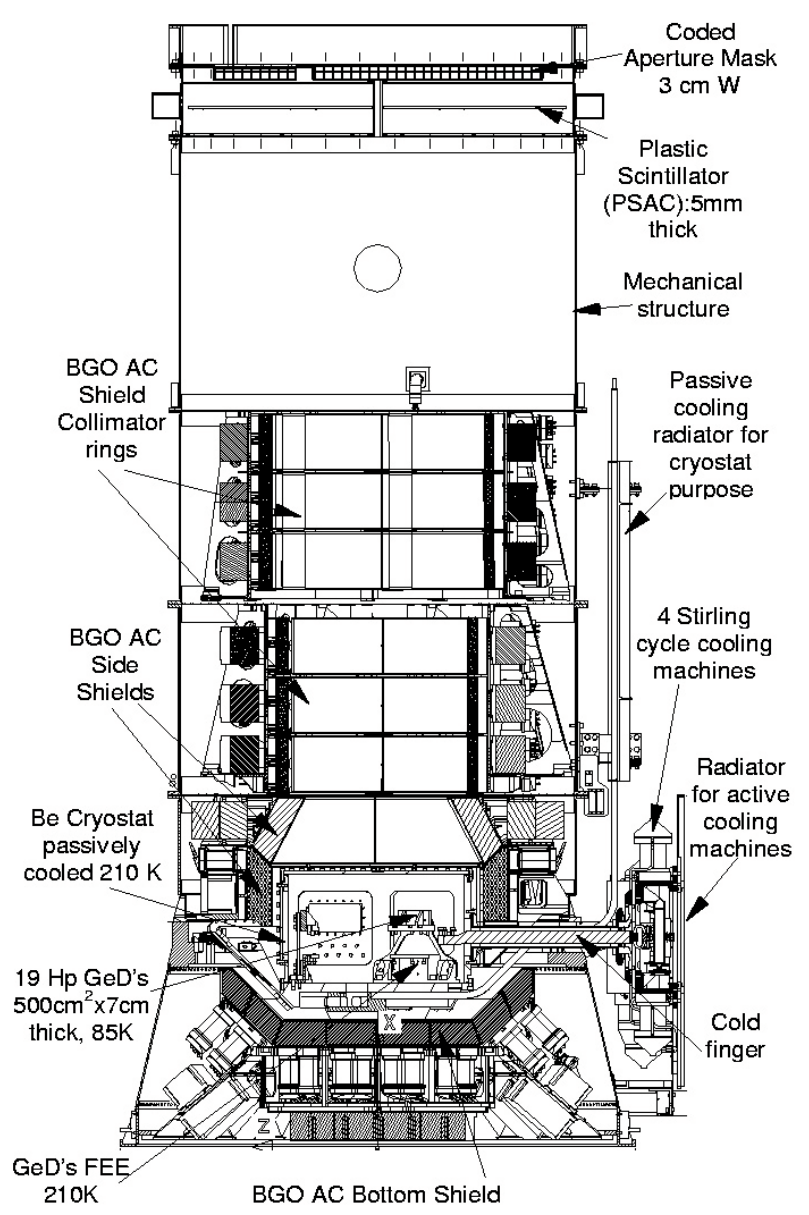
\includegraphics[width=\linewidth]{Images/General/SPI_cut_view_verdenne_2003.PNG}
  \vspace{-20pt}
  \caption{Cut-out view of the SPI spectrometer \cite{refId0}.}
  \vspace{-20pt}
  \label{SPI cut view}
\end{wrapfigure}


The INTErnational Gamma-Ray Astrophysics Laboratory (INTEGRAL) is an ESA space telescope with contributions from NASA and the RKA. Its mission began on October 17, 2002, when a Proton-DM2 rocket launched it from the Russian Baikonur spaceport in Kazakhstan into a 3-day, highly elliptical orbit with an apogee of 153000km and a perigee of 9000km, although this has not remained constant over the course of its lifetime. This places INTEGRAL mostly above radiation belts that would cause high instrumental backgrounds from charged-particle activation, and is why data collecting is halted during hours of close Earth-proximity. Initially, INTEGRAL had a 2+3-year planned lifetime, which it has greatly exceeded due to its lower than expected fuel consumption. Since then, its science operations have been repeatedly extended, currently up to the end of 2024, with some difficulties along the way such as its failed thrusters in July 2020 (compensated through the use of reaction wheels) and an uncontrolled tumbling caused by a single event upset in September 2021. The satellite is predicted to reenter Earth's atmosphere in 2029.



Onboard INTEGRAL are two main instruments: the Imager on-Board the INTEGRAL Satellite (IBIS) and the SPectrometer of INTEGRAL (SPI). IBIS specializes in being able to locate sources effectively. With an angular resolution of 12 arcmin, it can locate bright sources with arcmin precision in its $9^\circ \times 9^\circ$ field of view, and covers an energy range from 15keV to 10MeV. 

\subsection{About SPI}




SPI, the instrument used in this thesis and illustrated in figure \ref{SPI cut view}, specializes in its detailed energy resolution. At 1.3MeV, it is able to resolve energies with 2.5keV precision \cite{refId0}. It has a field of view of $16^\circ$ and an energy range covering 20keV to 8MeV. One decisive advantage SPI has in comparison to many comparable instruments is that its response matrices are based on extensive ground calibrations and Monte-Carlo simulations, as opposed to relying on astronomical sources such as the Crab Nebula \cite{2020ApJ...899..131J}.





\subsubsection*{Detectors}
SPIs detectors are composed of a hexagonal array of 19 reverse-electrode n-type germanium detectors. With a mean crystal weight of 951g and a mean volume of $178\text{cm}^3$, the total geometrical area for a flux parallel to the axis is $508\text{cm}^2$. Under normal working conditions, a voltage of 4000V is applied to each detector independently and this voltage is variable between zero and 5000V \cite{refId0}.

The germanium detectors require temperatures below 100K to work effectively, preferably as low as 85K in order to slow the effects of radiation damage. To accomplish this, SPI is equipped with an active cryogenic system. The Ge detector array is fixed on a Be plate, which is placed inside the cryostat. The plate is connected to the Stirling cycle cryocoolers to provide active cooling \cite{refId0}. 

Despite the low temperatures and hexagonal design to reduce the probability of hole traps in the semiconductor, radiation damage will inevitably accumulate over the course of a year or more. To combat this issue the detectors can undergo an annealing process, in which they are held at a temperature of $105^\circ \text{C}$ over the course of one or two days, depending on the damage. An annealing process of two days is enough to fully recover the energy resolution after radiation damage leading to a 20\% increase in the FWHM at 1.3MeV \cite{refId0}.

Each detector is connected to a preamplifier, which outputs the charge integrated signal (proportional to the measured energy) and the PSD signal (see below) to the detectors respective electronic chains for processing.

\subsubsection*{Pulse Shape Discrimination electronics (PSD)}



In order to suppress background events, SPI is equipped with Pulse Shape Discrimination (PSD) electronics. The idea is that localized beta decays in the detector material, which would otherwise be indistinguishable from photon energy deposits, only interact in a small volume of the detector, resulting in a single current pulse in the preamplifier. Gamma-rays, which primarily deposit energy via multiple compton scatterings in the detector volume, thus lead to a broader signal \cite{refId0}. 

Each detector is connected to its own PSD electronic system, which is only triggered in a certain energy range. The lower level threshold (LLD) is configurable, and has been varied between 400keV and 750keV over the mission's lifetime, where as the upper level threshold (ULD) is fixed at around 8MeV. Naturally, processing and analyzing the shape of a signal takes a certain amount of time, and when another event is measured within this time it is stored without any PSD information. The PSD electronics thus have an efficiency that can be approximated around 85\% \cite{Roques}.



\subsubsection*{Anticoincidence shield (ACS)}

\begin{wrapfigure}{R}{0.30\textwidth}
  \vspace{-20pt}
  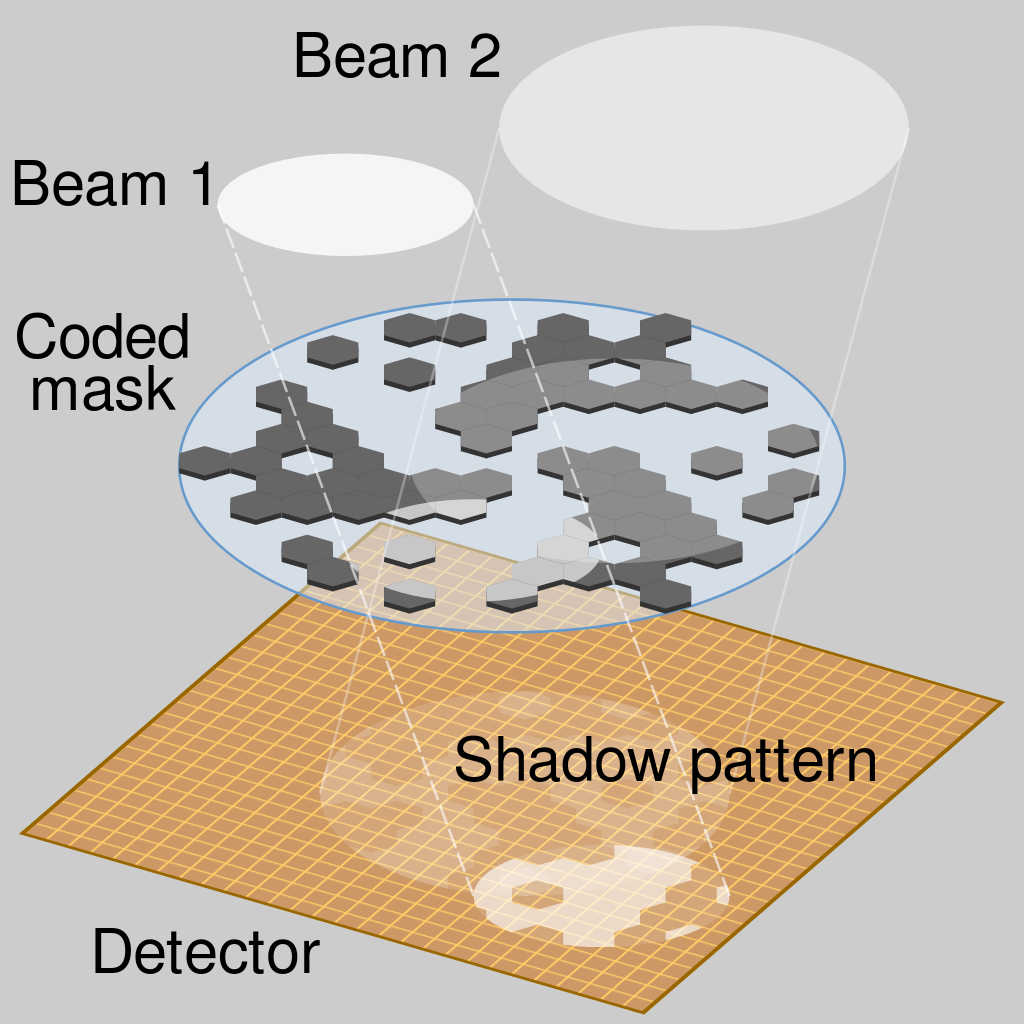
\includegraphics[width=\linewidth]{Images/General/HURA_hexagonal_coded_aperture_mask_principle.svg.png}
  \vspace{-20pt}
  \caption{The effect of SPIs mask on incoming source beams \cite{HURA}.}
  \vspace{-20pt}
  \label{HURA}
\end{wrapfigure}

To further prevent unnecessary background counts in the detectors an anticoincidence shield (ACS) is installed around various of SPIs components (see figure \ref{SPI cut view}). It consists of 91 BGO crystals with a volume of approximately $790\text{cm}^3$ each. Whenever an event is measured simultaneously in the ACS and in the Ge detectors it is vetoed \cite{refId0}. 



\subsubsection*{Mask}



\begin{figure}
  \centering
  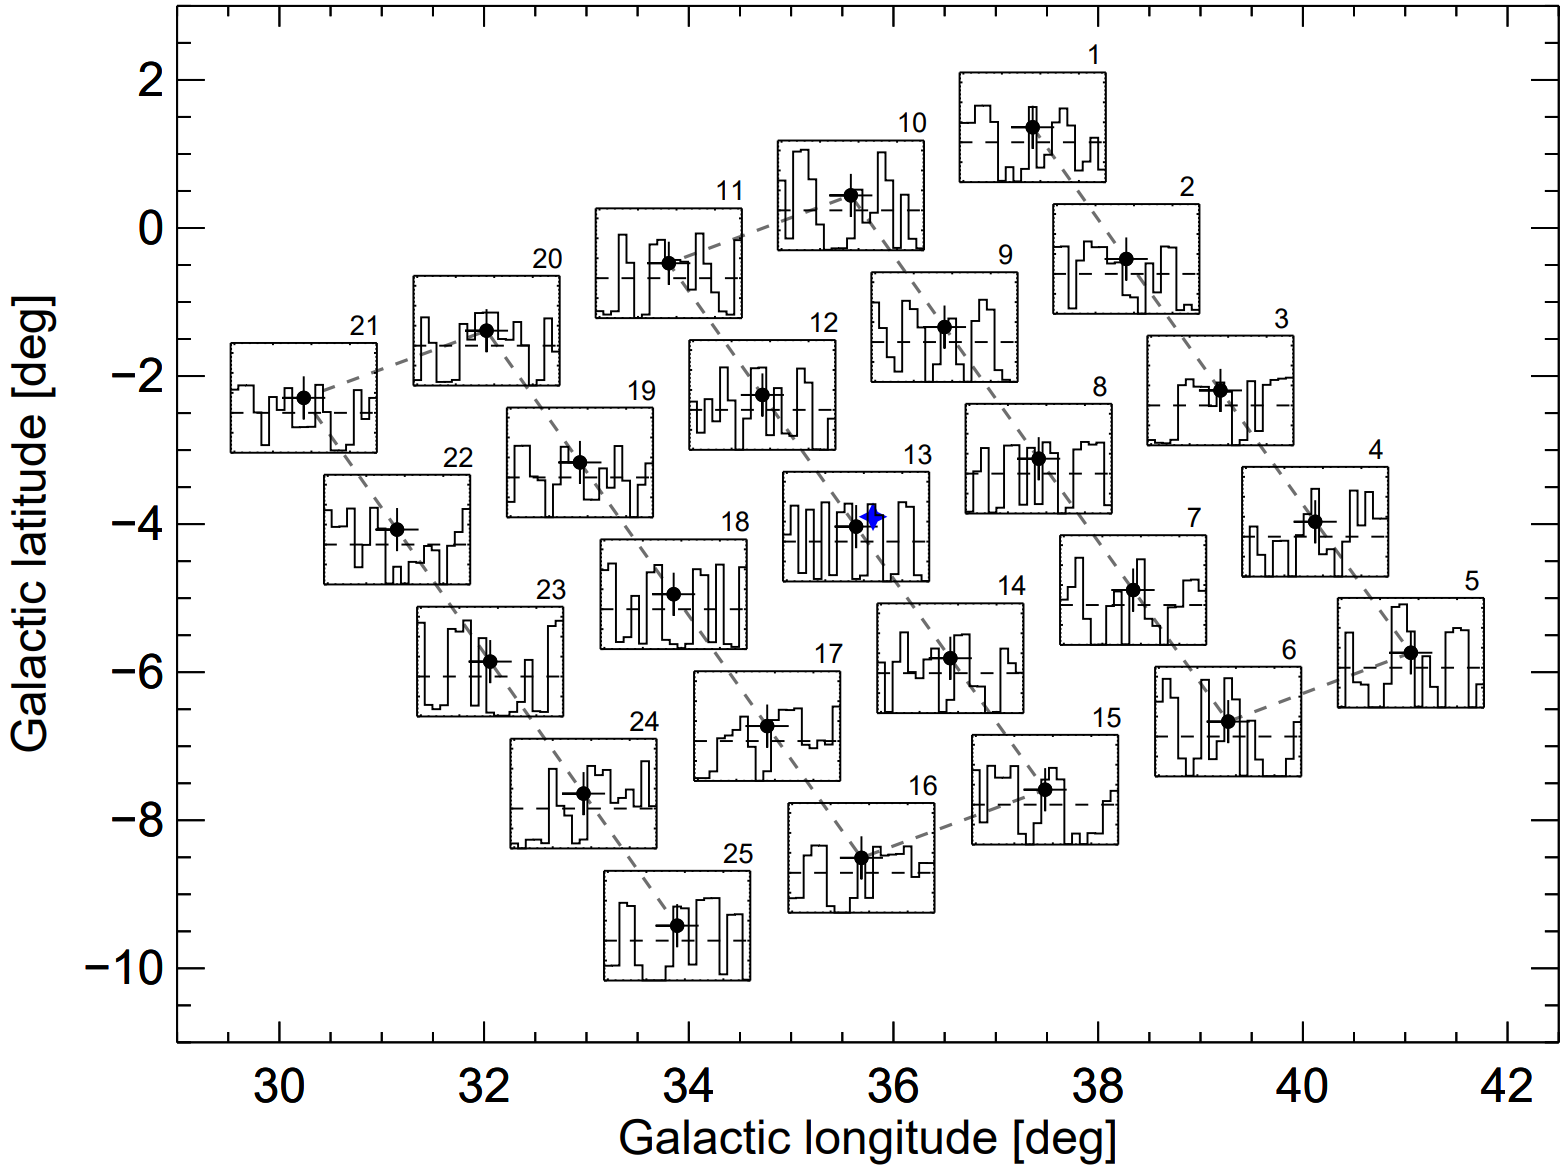
\includegraphics[width=\textwidth]{Images/General/Siegert_PHD_Pointings_pattern.PNG}
  \caption{A typical SPI $5\times5$ grid pointing pattern, each $2.1^\circ$ apart, marked with black dots and sequence number. The blue star in the center represents a celestial source, and the inset panels show the relative detector patterns from the celestial source. A close-up of pointing 13 is shown in figure \ref{spegert_pointings_pattern_close_up}. \cite{dissertation}}
  \label{spegert_pointings_pattern}
\end{figure}

\begin{figure}
  \centering
  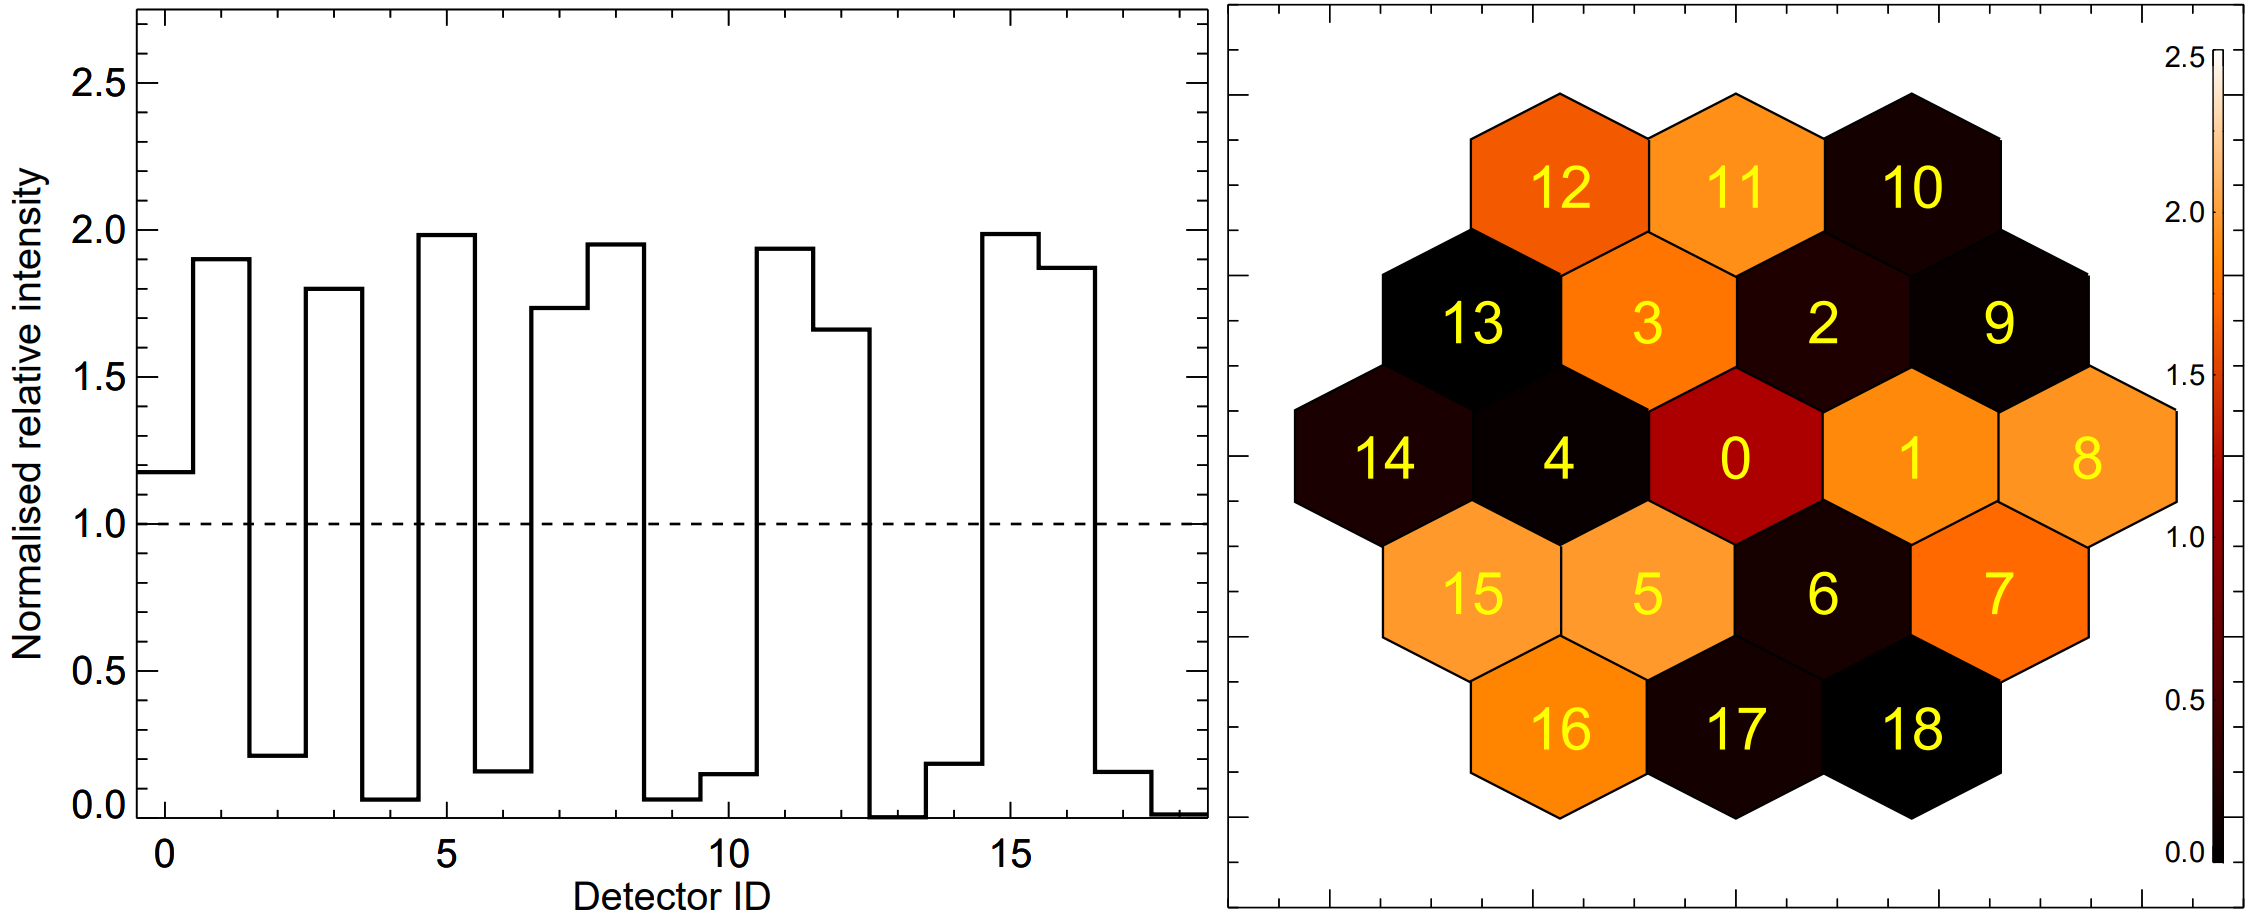
\includegraphics[width=\textwidth]{Images/General/Siegert_PHD_P13.PNG}
  \caption{A close-up of pointing 13 from figure \ref{spegert_pointings_pattern}. On the left we see the relative detector pattern caused by the source in a step plot, and on the right we see the same information displayed as a shadowgram on the detector array. \cite{dissertation}}
  \label{spegert_pointings_pattern_close_up}
\end{figure}

Before any photons can reach the array of detectors, they must pass through the coded aperture mask made of a 3cm thick tungsten alloy, located 1.71m above the detector plane. The $120^\circ$ rotationally symmetric mask is composed of 127 hexagonal tiles (63 opaque and 64 transparent to gamma radiation in the operating energy range) measuring 60mm side to side, and is inscribed within a circle with 720mm diameter \cite{refId0}. The effect that the mask has on incoming source beams is illustrated in figure \ref{HURA}, and the way this might influence the number of source counts measured in the detector array is visualized for an example source in figures \ref{spegert_pointings_pattern} and \ref{spegert_pointings_pattern_close_up}. This illustrates how we may infer both the source spectrum and position from the detector counts using multiple offset pointings of an astronomical source.




\subsubsection*{Event Types}
\begin{wrapfigure}{R}{0.55\textwidth}
  \vspace{-20pt}
  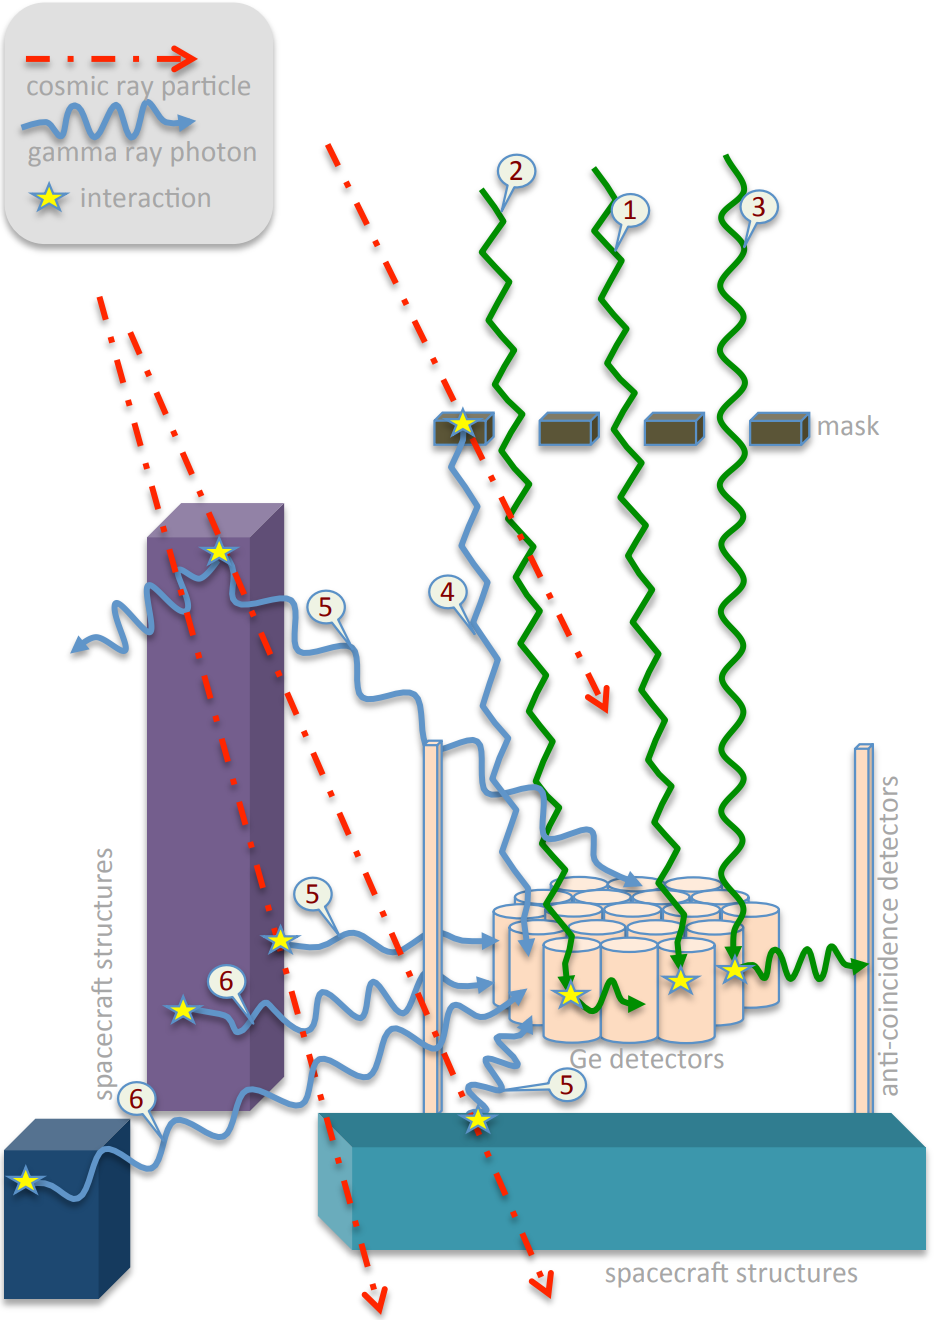
\includegraphics[width=\linewidth]{Images/General/SPI_event_types_roland_2017.PNG}
  \caption{Illustrations of different event types measured by SPI. Incoming source photons (green) may be absorbed in one detector (1), multiple detectors (2), or be self-vetoed by interacting with the ACS (3). Cosmic particles may interact with surrounding structures, resulting in background photons (blue)(4,5,6). Although the ACS helps suppress these events, they still occur. \cite{refId2}}
  \vspace{-50pt}
  \label{event_types}
\end{wrapfigure}

Figure \ref{event_types} shows some of the different event types measured by SPI. These are generally classified in the following categories \cite{Roques}:

\begin{itemize}
  \item Single Events (SE) - only one of the Ge detectors measured an energy deposit in the relevant time frame. Ideally this photon is fully absorbed in the detector, although there is no way of confirming this.
  \item Multiple Events (ME) - multiple Ge Detectors measured an energy deposit simultaneously. Ideally this is caused by a photon compton scattering to another detector (or multiple detectors), where it is fully absorbed. Again, there is no way of confirming this the photon is fully absorbed or that the measured energies were not coincident from multiple sources.
  \item Pulse Shape Discriminated Events (PE) - A SE for which the PSD electronics also triggered. Since each detector is equipped with its own PSD electronics chain, only SEs can be pulse shape discriminated. Another effect of this implementation is that the SE spectrum will have a reduced count rates in the PSD energy range, where SEs are PSD flagged and thus "removed" from the SE spectrum. 
\end{itemize}

Although the ACS does help with suppressing background and non-fully absorbed photons, it cannot guarantee  anything. In fact, a very large portion of SPIs measured counts are background counts. 

\subsubsection*{Spurious Events} \label{sec spurious events}
SPI also suffers from so called spurious events. These may occur when high-energy deposits are made in the germanium detectors. The analog electronics can become saturated and, due to reasons better explained elsewhere \cite{Roques}, low energy counts will be displaced toward higher energies. However, it has been found that the PSD electronics chain does not suffer from the same issues. This is why it is recommended to use only PEs in the PSD energy domain, and not SEs \cite{Roques}. 


\subsection{Astrophysics with SPI} \label{sec astrophysics with SPI}

The design choices of INTEGRAL SPI have been made specifically with its scientific objectives in mind. Those can be broken down into the study of three general categories: stellar evolution and nucleosynthesis, the interstellar medium, and compact objects. These can include both emission lines and contiuum processes. A small (and incomplete) selection of examples of how SPI can be used to study these is discussed below.

\subsubsection*{Stellar Evolution and Nucleosynthesis}
The abundance and distribution has changed greatly throughout the Universe's lifetime. Initially composed of many light elements, the synthesis of heavier elements in all stages of stellar evolution has led to today's distribution encompassing many heavier elements. This includes a wide array of unstable isotopes. SPIs high-precision energy resolution is excellent for detecting gamma-ray emissions from these isotopes. This information is extremely valuable to the scientific community as it gives crucial insight that may confirm or deny different theories on the processes that describe stars and thereby dictate particle physics.

Nucleosynthesis can occur in stars, novae, and supernovae. Each will have different distributions of decaying isotopes, which can be distinguished using SPI. Novae, for example, which occur in binary systems consisting of a white dwarfs accreting matter, will include the isotopes $^{13}$N, $^{18}$F, $^{7}$B, $^{2}$Na, and $^{26}$Al according to models which can be tested using SPI \cite{Wunderer2002ImagingWT}. Supernovae, which mark the explosive disruption of a star, result in several isotopes such as $^{56}$Ni, $^{57}$Ni, and $^{44}$Ti, whose shorter lifetimes (in comparison to $^{26}$Al or $^{60}$Fe) allow them to be attributed to single supernovae events instead of being detectable as diffuse emission only. Being able to accurately detect the decay lines of $^{44}$Ti at 68keV, 78keV, and 1.16MeV are will give great insight into the dynamics of supernova remnants. $^{26}$Al or $^{60}$Fe are two isotopes with very long half-lives and hence diffuse emissions. $^{26}$Al is predicted to be produced mainly in massive stars and core-collapse supernovae, whereas $^{60}$Fe is thought to be produced in all types of supernova events. Studying the differences in distributions of these isotopes is a powerful constraint on models of galactic nucleosynthesis \cite{Wunderer2002ImagingWT}.

\subsubsection*{Interstellar Medium}

Another important application for INTEGRAL SPI is in the study of interstellar medium, composed of gas and dust. One example way of studying the interstellar medium is via the 511keV line, which occurs from the annihilation of an $e^+,e^-$ pair. Electrons, that can be found in the interstellar medium, will annihilate with positrons that could originate from isotopes that decay via emission of a position or from $\pi^+$ decays generated in collisions from cosmic rays and the interstellar medium. In the thin medium the positrons can travel large distances before being slowed enough to interact with an electron. Studying the distributions of the 511keV line therefore has the potential to provide insight on the nature of interstellar medium \cite{Wunderer2002ImagingWT}.

\subsubsection*{Compact Objects}
Compact objects describe locations with high-energy processes and are thus of interest to test the limits of many physical laws and theories. Microquasars and active galactic nuclei are predicted to emit energetic positrons in their jets. These would again contribute to the 511keV line previously mentioned, but would be localized to point-like positions in the sky. Cyclotrons with strong magnetic fields can also be a source of monoenergetic gamma-ray emissions \cite{Wunderer2002ImagingWT}. 


This very short list of uses for INTEGRAL SPI gives but a glimpse into the many scientific discoveries that become possible using the data collected by SPI.

\section{About Spimodfit} \label{about smf}



Given the complexities discussed above, and many more not discussed, it is clear that working with SPI data is no trivial task. Although SPIs Instrument Response Function (IRF) is readily available to be used, there is no stand-alone background model. Since the background counts dominate source counts in almost all circumstances, it is no surprise that several independent methods to analyze SPI data have been developed. One such method is Spimodfit, developed primarily by Andy Strong, Hubert Halloin, and Thomas Siegert at MPE \cite{refId1} \cite{SMF_Cookbook}.

\begin{wrapfigure}{R}{0.55\textwidth}
  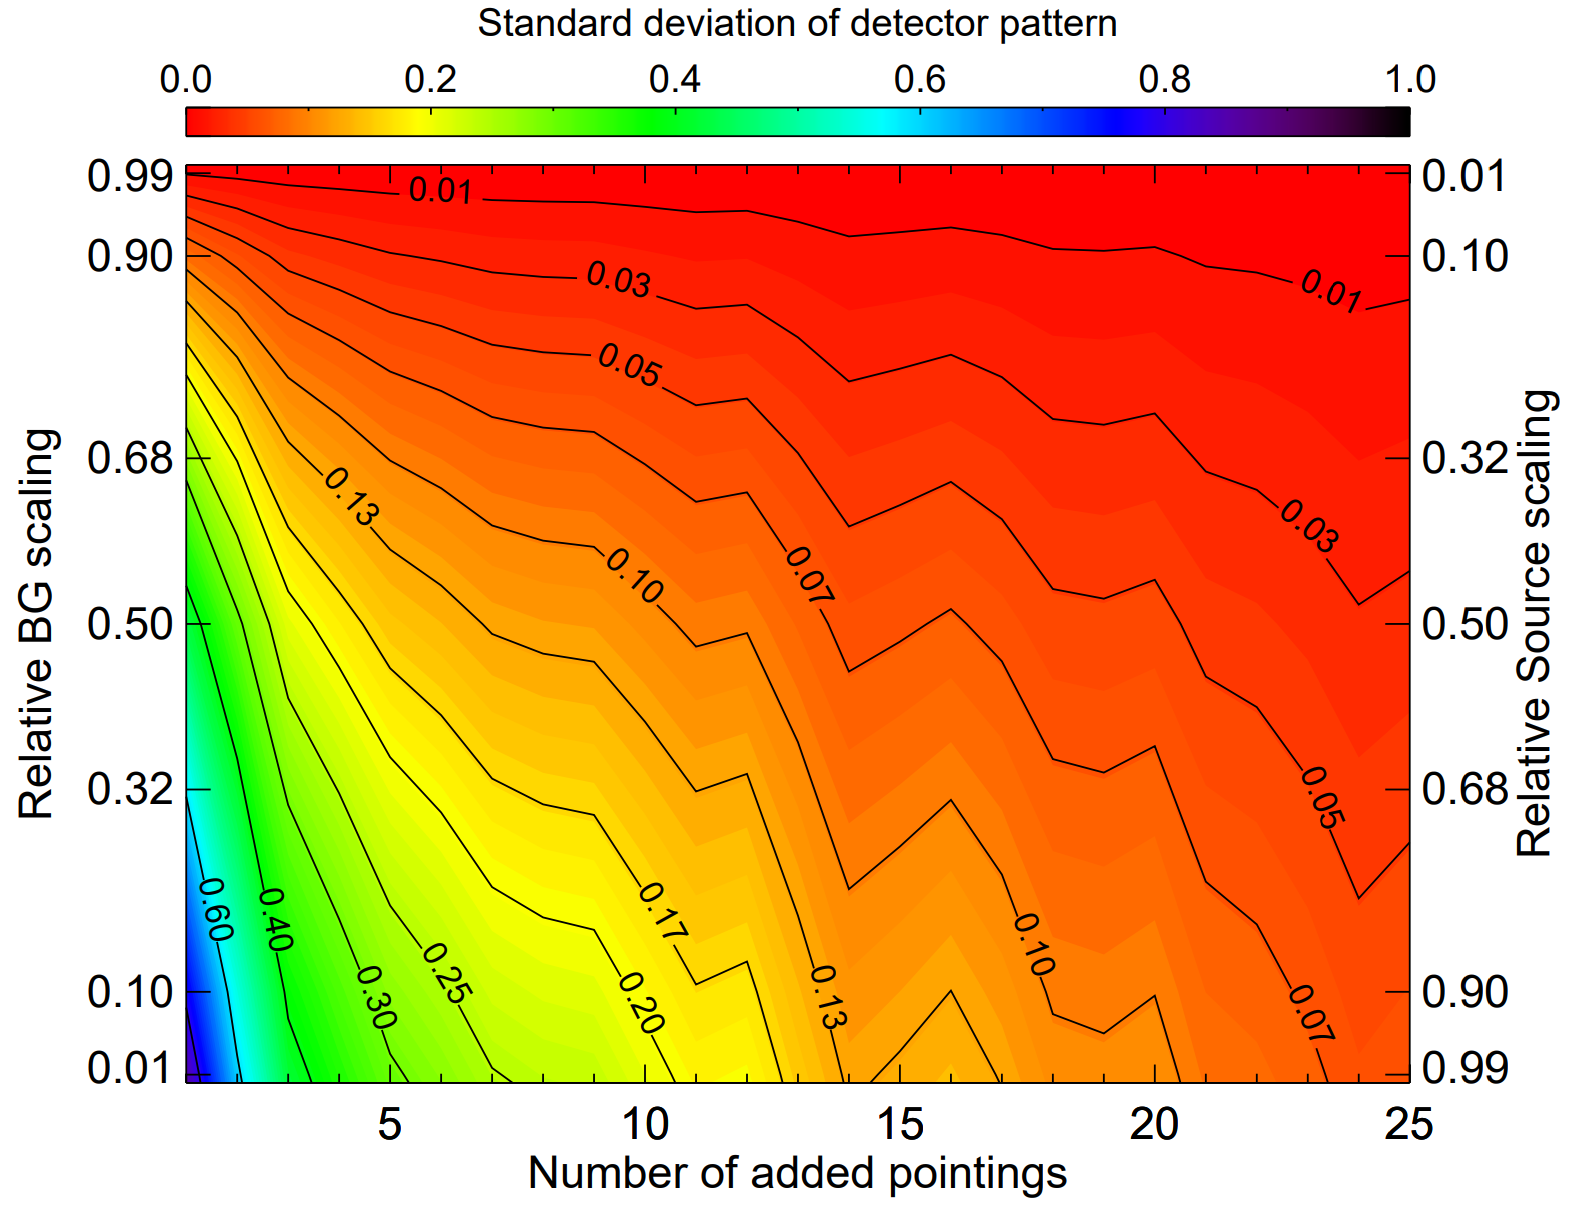
\includegraphics[width=\linewidth]{Images/General/SMF_background_pattern_siegert_2019.PNG}
  \caption{The standard deviation of detector patterns as a function of the number of pointings and the source to background intensity. We see that even very bright sources become almost entirely washed out given enough pointings, and only the sum of the background detector patterns remains. \cite{refId1}}
  \vspace{-0pt}
  \label{smf_background_model_idea}
  \vspace{-35pt}
\end{wrapfigure}

In order to create Spimodfit a detailed background and response database had to be constructed first. The fundamental idea that allows this background database to work is that the detector count-rate patterns of individual isotopes stay constant on all timescales. This means that every process that leads to background counts creates some specific, energy dependent pattern in the detector array which stays constant. These processes are split into parameters for continuum processes as well as many $\gamma$-ray lines. The intensities of these different patterns created by the processes may vary, which is why they are fitted to the relevant count-spectra per energy bin in order to create the background spectrum used in every analysis. This requires one to have knowledge of what the different patterns are. Hence, a database of the detector patterns was created by adding many SPI pointings together over relevant timescales, so that any sources in the pointings are washed out and only the detector patterns remain (see figure \ref{smf_background_model_idea}). Naturally, this very brief description of the Spimodfit background model given here skips over many details and complexities that had to be taken into consideration.

Spimodfit will be used extensively in this thesis as a reference point regarding SPI data fitting.



\section{PySPI and the Goal of this Thesis}
PySPI is a python analysis framework for Gamma-Ray Burst (GRB) data from SPI, developed primarily by Björn Blitzinger at MPE \cite{Biltzinger2022}. It is designed to take user inputs like the time of the GRB and energy bins, automatically download relevant data files, and to construct a response and time series, which can then be used as a plugin for 3ML \cite{3ml}.

Momentarily, PySPI is only built to work with transient sources. The goal of this thesis is to extend PySPIs functionality to be able to analyze persistent sources as well. Unlike transient sources, whose time-sensitive nature circumvents the need for an accurate background description, persistent sources are not so easily distinguished from background counts and thus do necessitate a way to deal with SPIs dominant background.

The design and implementation this method is motivated by the many possible applications for SPI data (section \ref{sec astrophysics with SPI}). Although previous methods like Spimodfit exist and work, the inherent difficulties of extracting a source flux given the dominant background mean that any method of modeling the background spectrum will have natural flaws. The exact extend of these flaws is unknown, which is why the creation of a fundamentally different approach of dealing with SPI data will offer crucial insight into the shortcomings of previous methods.

The methodology implemented in this thesis was developed in collaboration with Björn Blitzinger and Jochen Greiner.

\chapter{Theory and Simulation}

\section{General Procedure} \label{General Procedure}
In contrast to previous approaches to working with INTEGRAL SPI, the method of analyzing SPI data developed for this thesis does not attempt to construct a background model, and instead uses a profile likelihood to eliminate its effect in the source model fit. The underlying assumption that allows this to work is that background count rates in each energy bin per detector remain constant for temporally and spatially near SPI Science Windows (SCWs) (also called pointings). As figure \ref{event_types} illustrated, background counts mostly originate when photons or other particles first interact with non-detector material of the satellite, and then find their way into the detectors via scattering, de-excitation, etc. These interactions heavily diffuse any angular dependance of the original source of the background event toward SPIs orientation. Furthermore, only in very rare circumstances (solar flares, etc.) will the rate of background events change on short time scales. This justifies the assumption that most neighboring SCWs with mere minutes or hours of time difference and only a few degrees difference in SPIs orientation will have identical background count rates. 

Neighboring SCWs are thus grouped into clusters of assumed constant background count-rates, allowing for a source model to be fitted to the data using the likelihood calculations described below. Just like in chapter \ref{Introduction}, we distinguish between source counts, which describe all detected events directly originating from astronomical objects considered in our source model, and background counts, which describe all other detector events.

\subsection{Likelihood Calculation}

Once we have split our set of SCWs into clusters within which we claim the assumption of constant background to be true and have defined a source model, a likelihood value can be calculated for each energy bin of each detector in each cluster. If one energy bin of one detector in one SCW with measuring time $t$ has a source count rate $s$ and a background count rate $b$, the probability $P$ of measuring $C$ counts follows a Poisson distribution:
\begin{equation}
    P(C \vert b, s, t) = \frac{\left( t \left( b + s \right) \right) ^C \text{exp}\left( -t \left( b+s\right)\right)}{C!}
\end{equation}

Equivalent energy bins in the same cluster are assumed to have the same background count rate $b$, so that the probability of measuring $C_1$ counts in one SCW and $C_2$ counts in another SCW is simply:

\begin{equation} \label{eq probs}
    P(C_1, C_2 \vert b, s_1, t_1, s_2, t_2) = P(C_1 \vert b, s_1, t_1) \cdot P(C_2 \vert b, s_2, t_2)
\end{equation}

The likelihood $\mathcal{L}$ for any energy bin of a detector within a cluster depends on all equivalent energy bins in that cluster, i.e. one term for each SCW in the cluster. If we have cluster of size two, the likelihood is described by:

\begin{equation}\label{log likelihood}
    \text{ln}\mathcal{L}(C_1, C_2, t_1, t_2\vert b, s_1 s_2) = \text{ln}P(C_1 \vert b, s_1, t_1) + \text{ln}P(C_2 \vert b, s_2, t_2)
\end{equation}

To proceed further we require the probability distribution of $b$. A full and mathematically correct treatment of the background parameter $b$ involves  turns out to be very cumbersome with only marginal benefits. Hence, the profile likelihood is used by simply solving for the background count rate value $b_M$ which maximizes the likelihood. This is easily done by setting the derivative of equation \ref{log likelihood} to zero and solving for $b$. For a cluster size of two one finds:
\begin{equation} \label{eq: max lik back}
    b_M = \frac{1}{2} \left[ \frac{C_t}{t_t} - s_t + \sqrt{\left( \frac{C_t}{t_t} - s_t\right)^2 + 4 \left( \frac{C_1s_2+C_2s_1}{t_t}-s_1s_2\right)}\right]
\end{equation}
where $C_t=C_1+C_2$, $s_t=s_1+s_2$, and $t_t=t_1+t_2$. Using this maximum likelihood background $b_M$ finally allows us to compute a likelihood value that is only dependent on the measured counts and the source model:
\begin{equation} \label{log_likelihood final}
    \text{ln}\mathcal{L}(C_1, C_2, b_M, t_1, t_2 \vert s_1, s_2) = \text{ln}P(C_1 \vert b_M, s_1, t_1) + \text{ln}P(C_2 \vert b_M, s_2, t_2)
\end{equation}
The process for clusters with sizes larger than two is analogous. One such likelihood value exists for every energy bin of every detector in every cluster, such that the total likelihood value for any given source model is simply the sum of the logarithmic likelihoods over all energy bins, detectors, and clusters:

\begin{equation} \label{total log likelihood}
  \text{ln}\mathcal{L}_{\text{total}} = \sum_{\text{Clusters}}\sum_{\text{Detectors}}\sum_{\text{Energy-Bins}} \text{ln}\mathcal{L}(C_1, C_2, b_M, t_1, t_2 \vert s_1, s_2)
\end{equation}

A suitable algorithm, such as Multinest, \cite{Feroz_2019} may be applied to determine the posterior probabilities of the source model parameters based on this likelihood.
Multinest is an implementation of a Bayesian inference algorithm. For a model $M$ with parameters $\Theta$ and data $D$, Bayes theorem states that
\begin{equation}
  P(\Theta\vert D, H) = \frac{P(D\vert \Theta, H)P(\Theta\vert H)}{P(D\vert H)}
\end{equation}
where $P(\Theta\vert D, H)$ is the posterior probability distribution of the parameters, $P(D\vert \Theta, H)$ is the likelihood ($\mathcal{L}_{\text{total}}$ in our case), $P(\Theta\vert H)$ is the prior, and $P(D\vert H)$ is the Bayesian evidence. The Bayesian evidence is the factor required to normalize the posterior:
\begin{equation}
  P(D\vert H) = \int P(D\vert \Theta, H) P(\Theta\vert H) \text{d}^D \Theta
\end{equation}
where $D$ is the dimensionality of the parameters space. Nested sampling is the method implemented in Multinest to solve this complex multidimensional integral. It uses an ensemble of live points, replacing the lowest likelihood points with new points to narrow the result down and evaluate the integral in horizontal slices \cite{Feroz_2019}.

The complexity of this procedure is why we are forced to rely on the profile likelihood for parameter instead of a full and mathematically correct description of the background, which would involve solving equation \ref{eq probs} for $b$:
\begin{equation}
  P(b \vert C_1, C_2, s_1, t_1, s_2, t_2) = \frac{P(C_1, C_2 \vert b, s_1, t_1, s_2, t_2)}{\int_{-\infty}^{\infty} P(C_1, C_2 \vert b, s_1, t_1, s_2, t_2) \text{d}b}
\end{equation}
The extra dimensionality this introduces in the nested sampling algorithm is virtually impossible to overcome with modern hardware limitations.


An important detail is that the expected value of the maximum likelihood background is equal to the true background rate:
\begin{equation}
  E(b_M) = b
\end{equation}
Depending how the random samples of the poisson distributions are drawn, it is possible for the maximum likelihood background to be less than zero $b_M<0$. One might be tempted to impose a lower limit of 0 since the physical background rate cannot be lower than 0, but this would actually be a big mistake. The introduced asymmetry would mean that the expected value of the maximum likelihood background is no longer equal to the true rate $E(b_M) \neq b$, which in turn prevents a bayesian fitting algorithm from correctly determining the true source parameters. Testing has conclusively shown that introducing such a lower limit results in significant systematic errors of the fit.


\subsection{General Procedure: Summary}

The general procedure for fitting persistent sources with PySPI can thus be summarized in the following steps:
\begin{enumerate}
  \item Select all relevant SCWs to be used in the analysis. Usually this is done on a revolution basis, so that all SCWs from the used INTEGRAL revolutions are included, provided SPIs orientation is sufficiently close to the source in question.
  \item Group the relevant SCWs into clusters. These should preferably have only a small time difference and angular distance in SPIs orientation between them so that the assumption of a constant background rate in every energy bin of every detector is justified. Refer to appendix \ref{Clustering Algorithm} for more details on the clustering algorithm developed for this purpose. In principle, clusters of any size ($>1$) can be used, although only cluster-sizes 2 and 3 have been implemented and tested. Clusters of size 2 are most commonly used since they are generally the easiest to work with due to the constant background assumption and computational speeds.
  \item Set-up a source model to be fitted to the data using the python package astromodels \cite{astromodels}. The built in SPI response function capabilities of PySPI allow one to easily calculate the count rates based on the model.
  \item Set-up equation \ref{total log likelihood} so that the multinest bayesian fitting algorithm can vary the source model parameters to maximize the total likelihood. Then run the fit.
  \item If deemed necessary conduct a posterior predictive check (PPC) analysis (see chapter \ref{sec:PPC Back}) to verify the the fit quality and check if the assumption of constant background rates is well met. It is a common occurrence for some clusters to not have constant (or constant enough) background rates. These are easily identified in the PPC CDFs, so that they may be removed from the list of clusters for the fit to be run again.
\end{enumerate}



\section{Pure Simulation}\label{sec: pure sim}
Before any real sources are fitted, it is mandatory to test the SPI fitting method on a purely simulated count spectrum. This not only allows us to see exactly how well the fit performs since we know the true model parameters of any sources in the simulated spectrum, but it also allows us to test under which conditions the fit may or may not fail.

To begin, a simulated count spectrum is required, consisting of source and background counts. For the following simulations this is done in the following way, unless otherwise specified:

\begin{enumerate} 
  \item Choose a real SPI revolution as a baseline. It is mostly irrelevant which revolution is chosen. For this analysis revolution 0374 is used. We will use the SPI orientations of the SCWs in this revolution as the orientations of our simulated SCWs in order to achieve realistic conditions. 
  \item \label{step pure sim back}Generate a background spectrum. In order to have a realistic background spectrum, the background counts from one SCW are taken and duplicated to all other SCWs and then poisson distributed. The lifetimes (total active measuring time of each detector in each SCW) for each SCW are also duplicated correspondingly. This way the background count rates are identical for all SCWs, yet also realistic, in the sense that the spectrum could be that of an actual SPI SCW.
  \item Define the spectrum of the source to be simulated, as well as position. In this case powerlaws as shown in equation \ref{powerlaw} are used, and the position of the sources is chosen to be central to as many SCWs in the revolution as possible ($RA=10^\circ, DEC=-40^\circ$ in equatorial coordinates). Although the exact parameters used in the following sections will vary, most powerlaw spectra are chosen to be comparable to the Crab Nebula in terms of luminosity and index.
  \item Use the SPI Instrument Response Function (IRF) to calculate the expected source count rates in each energy bin in each detector for each SCW. Multiply these by the respective lifetimes of the detectors in the SCWs, and finally draw a sample of a Poisson distribution with the respective means to attain the measured counts of the simulated source for each energy bin in each detector in each SCW.
  \item Add the source counts to the background counts to acquire the total counts.
\end{enumerate}

To measure the quality of a fit we shall use the Mahalanobis distance:

\begin{equation}
  d_M = \sqrt{(\vec{V}_F - \vec{V}_T)^TS^{-1}(\vec{V}_F-\vec{V}_T)}
\end{equation}

which tells us the number of standard deviations the fitted source values $\vec{V}_F$ are away from the true source values $\vec{V}_T$, where $S$ is the covariance matrix.

Unless otherwise specified, the following fits utilize an energy range of 18-2000keV. Since this is purely simulated data we do not need to worry about spurious events or any other anomalies in the SPI data-space. In order to visualize the results we may plot the confidence intervals of the posterior parameter distributions next to the true source parameters, which we know exactly due to having simulated the sources. Unless otherwise specified, the confidence intervals of one standard deviation are used.

\subsection{Consistency, Accuracy, and Precision}

\begin{figure}[h]
  \centering
  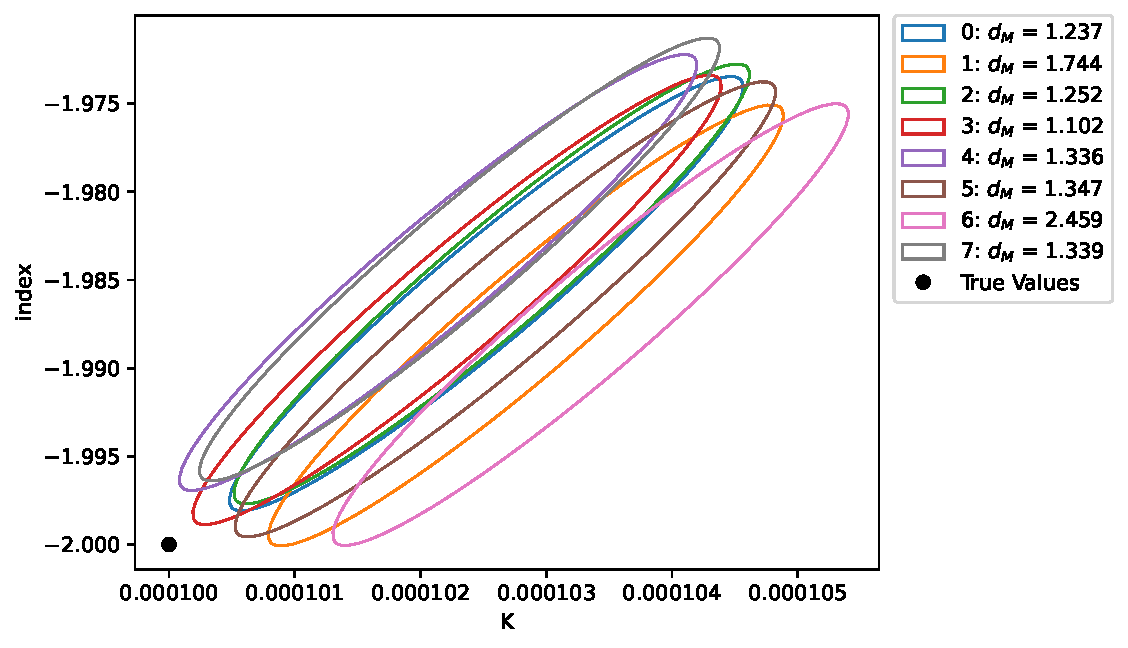
\includegraphics[width=\textwidth]{Images/Pure_Simulation/combined_plot_repeated_identical.pdf}
  \caption{Repeated fits for exactly identical datasets.}
  \label{fig ident}
\end{figure}

The first test is how consistent the fitting is with exactly identical inputs. The results are shown in figure \ref{fig ident}, where the same source is fitted 8 times. We see that the results are all very similar. However, since the inputs are exactly identical, it is surprising that the multinest fitting algorithm still has deviations this significant, ranging from 1.1 to 2.4 standard deviations away from the true values. 

\begin{figure}[h]
  \centering
  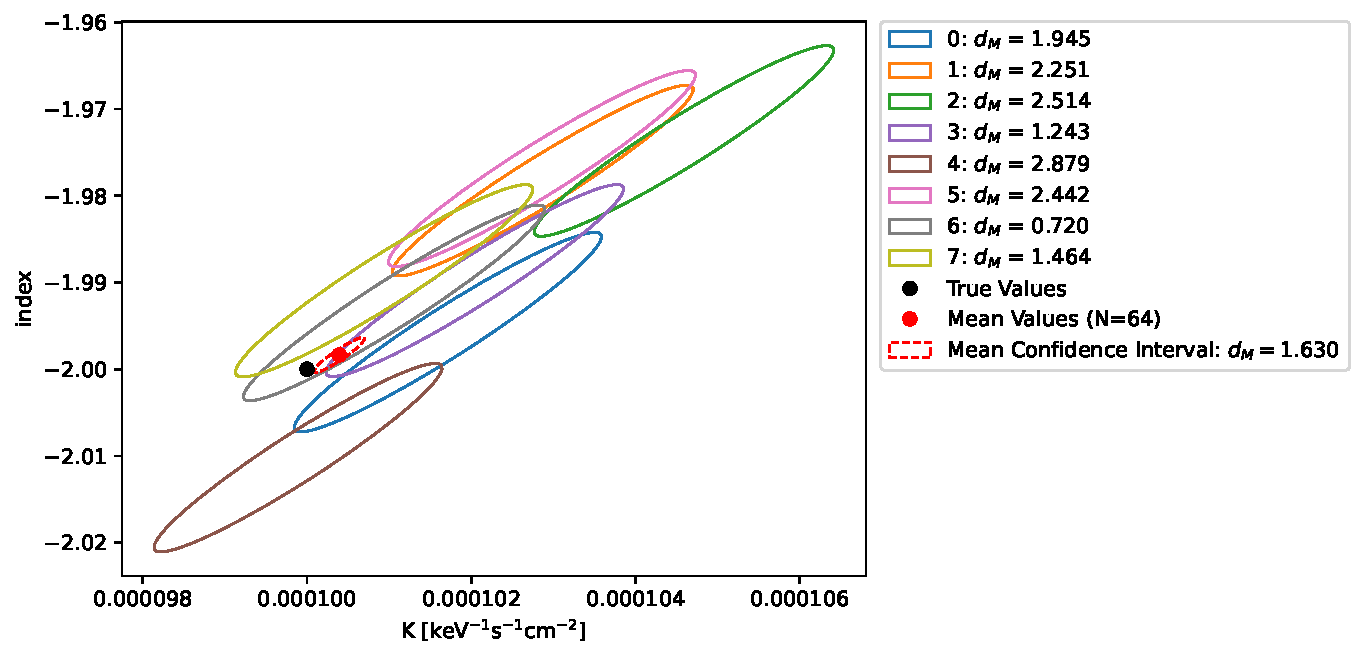
\includegraphics[width=\textwidth]{Images/Pure_Simulation/combined_plot_repeated_identical_new_gen.pdf}
  \caption{Repeated fits for newly generated datasets, using the same exact same baseline before random poisson samples are drawn in the dataset generation. Also shown is the mean fit value for 64 fits (only 8 shown here), as well as the confidence interval of said mean.}
  \label{fig ident new gen}
\end{figure}

Although the previous test gave us great insight into the consistency of the fits, it told us nothing about their accuracy. To test this we have to regenerate the simulated source spectrum, so that every random poisson sample is redrawn. The results of this are shown in figure \ref{fig ident new gen}. As expected, the results are now distribution with much greater variance around the true values. Based on the 8 fits shown, the suspicion of a systematic error may arise. This is why this process (generating a new count spectrum and fitting it) was repeated a total of 64 times. We see that the mean values of these 64 fits and the confidence interval of the mean (taking the sample variance and the variance of individual fits into consideration) match the true values well at 1.63 standard deviations distance. We may thus conclude that we do not have a statistically significant systematic error, at least for the parameters used to set-up this fit.


\begin{figure}[h]
  \centering
  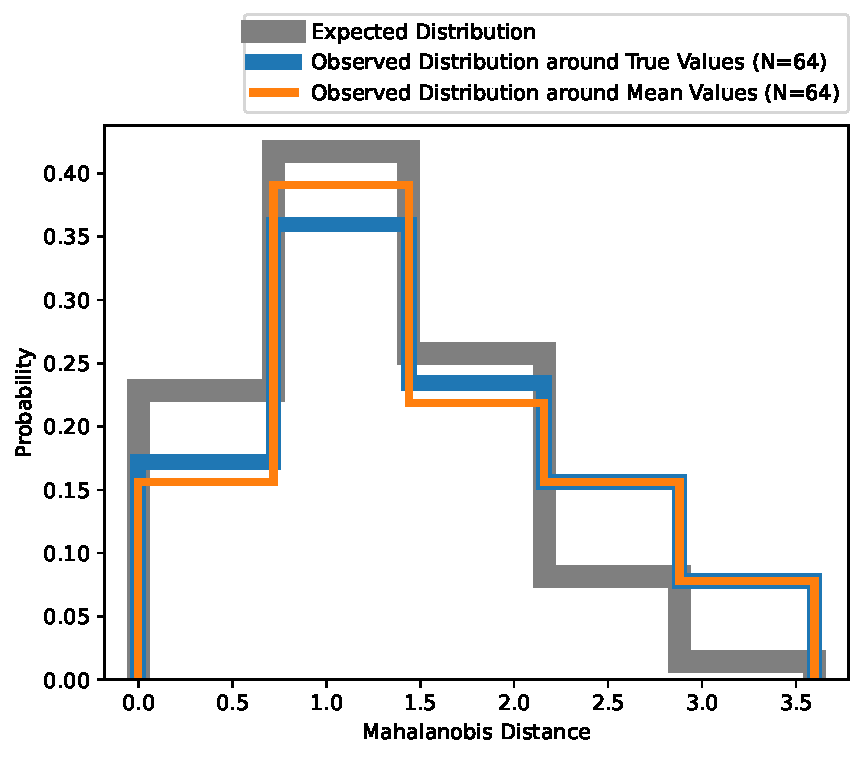
\includegraphics[width=0.60\textwidth]{Images/Pure_Simulation/d_M_distribution.pdf}
  \caption{The distribution of Mahalanobis distances from the 64 fits from figure \ref{fig ident new gen} compared to the expected distribution from equation \ref{d_M exp}. Also shown is the distribution of Mahalanobis distances around the mean values from the 64 fits, instead of the true values.}
  \label{fig d_M distribution}
\end{figure}


Finally, we want to test the precision of the fits, i.e. how well the uncertainties of the posterior parameters distributions match their distribution around the true values. Approximating the posterior distributions as gaussian (a fair assumption in this case), the probability of a two-dimensional fit to be between $x_1$ and $x_2$ standard deviations away from the true values is:
\begin{equation} \label{d_M exp}
  P(x_1<d_M<x_2) = \frac{\int_{x_1}^{x_2}x \text{exp}(-\frac{1}{2}x^2)\text{d}x}{\int_{0}^{\inf}x \text{exp}(-\frac{1}{2}x^2)\text{d}x} = \text{exp}(-\frac{1}{2}x_1^2) - \text{exp}(-\frac{1}{2}x_2^2)
\end{equation}
We may thus compare the distributions of the Mahalanobis distances from our 64 fits (figure \ref{fig ident new gen}) to the expected distributions, as is done in figure \ref{fig d_M distribution}. Although the distributions match fairly well, we do see a significant shift towards higher Mahalanobis distances than expected. It appears that our fitting procedure has has a slight tendency to underestimate its posterior uncertainties. That being said, a sample size of 64 is not large enough to definitively support this claim.

Figure \ref{fig d_M distribution} also shows the distributions of Mahalanobis distances around the mean values of the 64 fits, as opposed to the known true values. After Bessel correcting the fit variances to adjust for biases in the sample mean we see a nearly identical distribution, further supporting the claim that there is no systematic error in the fit. 

\FloatBarrier

\subsection{Energy Range}

\begin{figure}[H]
  \centering
  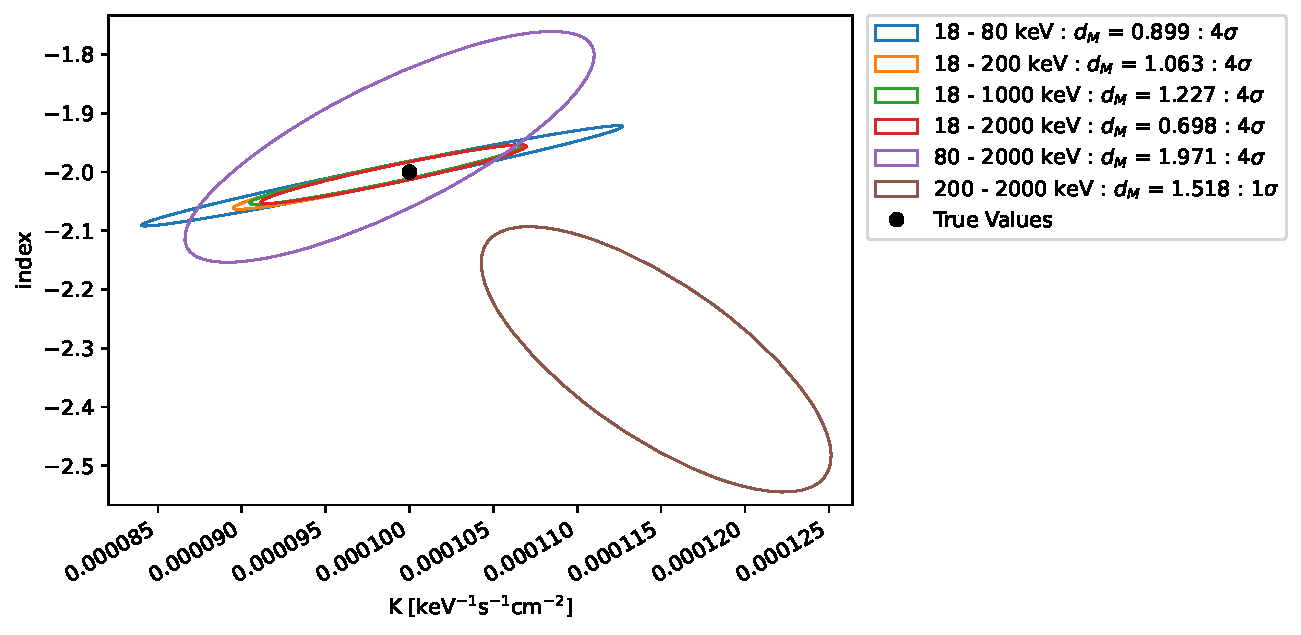
\includegraphics[width=0.9\textwidth]{Images/Pure_Simulation/combined_plot_energy_range.pdf}
  \caption{Identical dataset fitted using only the specified energy ranges. Also note the different number of standard deviations shown in the confidence intervals.}
  \label{fig energy range}
\end{figure}

Figure \ref{fig energy range} shows an identical dataset fitted using different energy ranges. The fits including the entire energy range of 18-200keV and beyond all deliver very similar results. When the energy range does not reach all the way to 200keV or does't begin at 18keV, the precision of the model parameter fits worsens drastically. Considering a Crab-like source will have its most relevant source counts below 200keV (see figure \ref{fig back spec}) this is not very surprising. It is also worth noting that despite the uncertainties of the fits showing large differences, the number of standard deviations from the true values remains comparable. Every single fit shown here uses 125 logarithmically spaced energy bins in the corresponding energy ranges.




\subsection{Number of Energy Bins}

\begin{figure}[h]
  \centering
  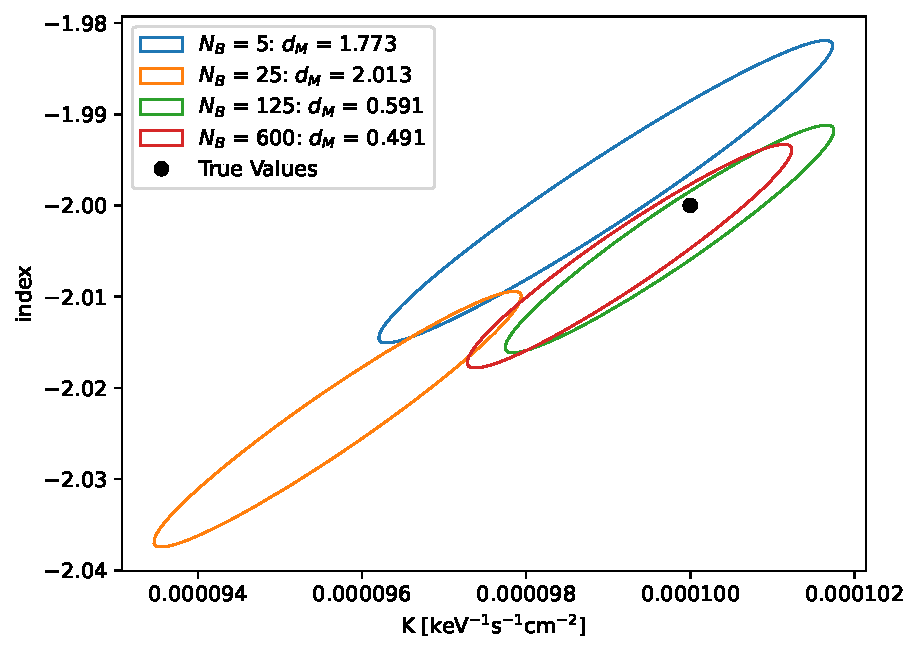
\includegraphics[width=0.55\textwidth]{Images/Pure_Simulation/combined_plot_num_e_bins.pdf}
  \caption{Identical dataset fitted using different numbers of energy bins $N_B$.}
  \label{fig num bins}
\end{figure}

Due to the decreasing number of counts from both source and background at higher energies, the spectra are re-binned into logarithmically spaced bins. Figure \ref{fig num bins} shows what happens when we vary the number of logarithmically spaced bins used. As one might expect, we see no significant differences, except that the uncertainty for 5 energy bins is very slightly larger than for the other fits.


\subsection{Fitting Different Powerlaws}

\begin{figure}[h]
  \centering
  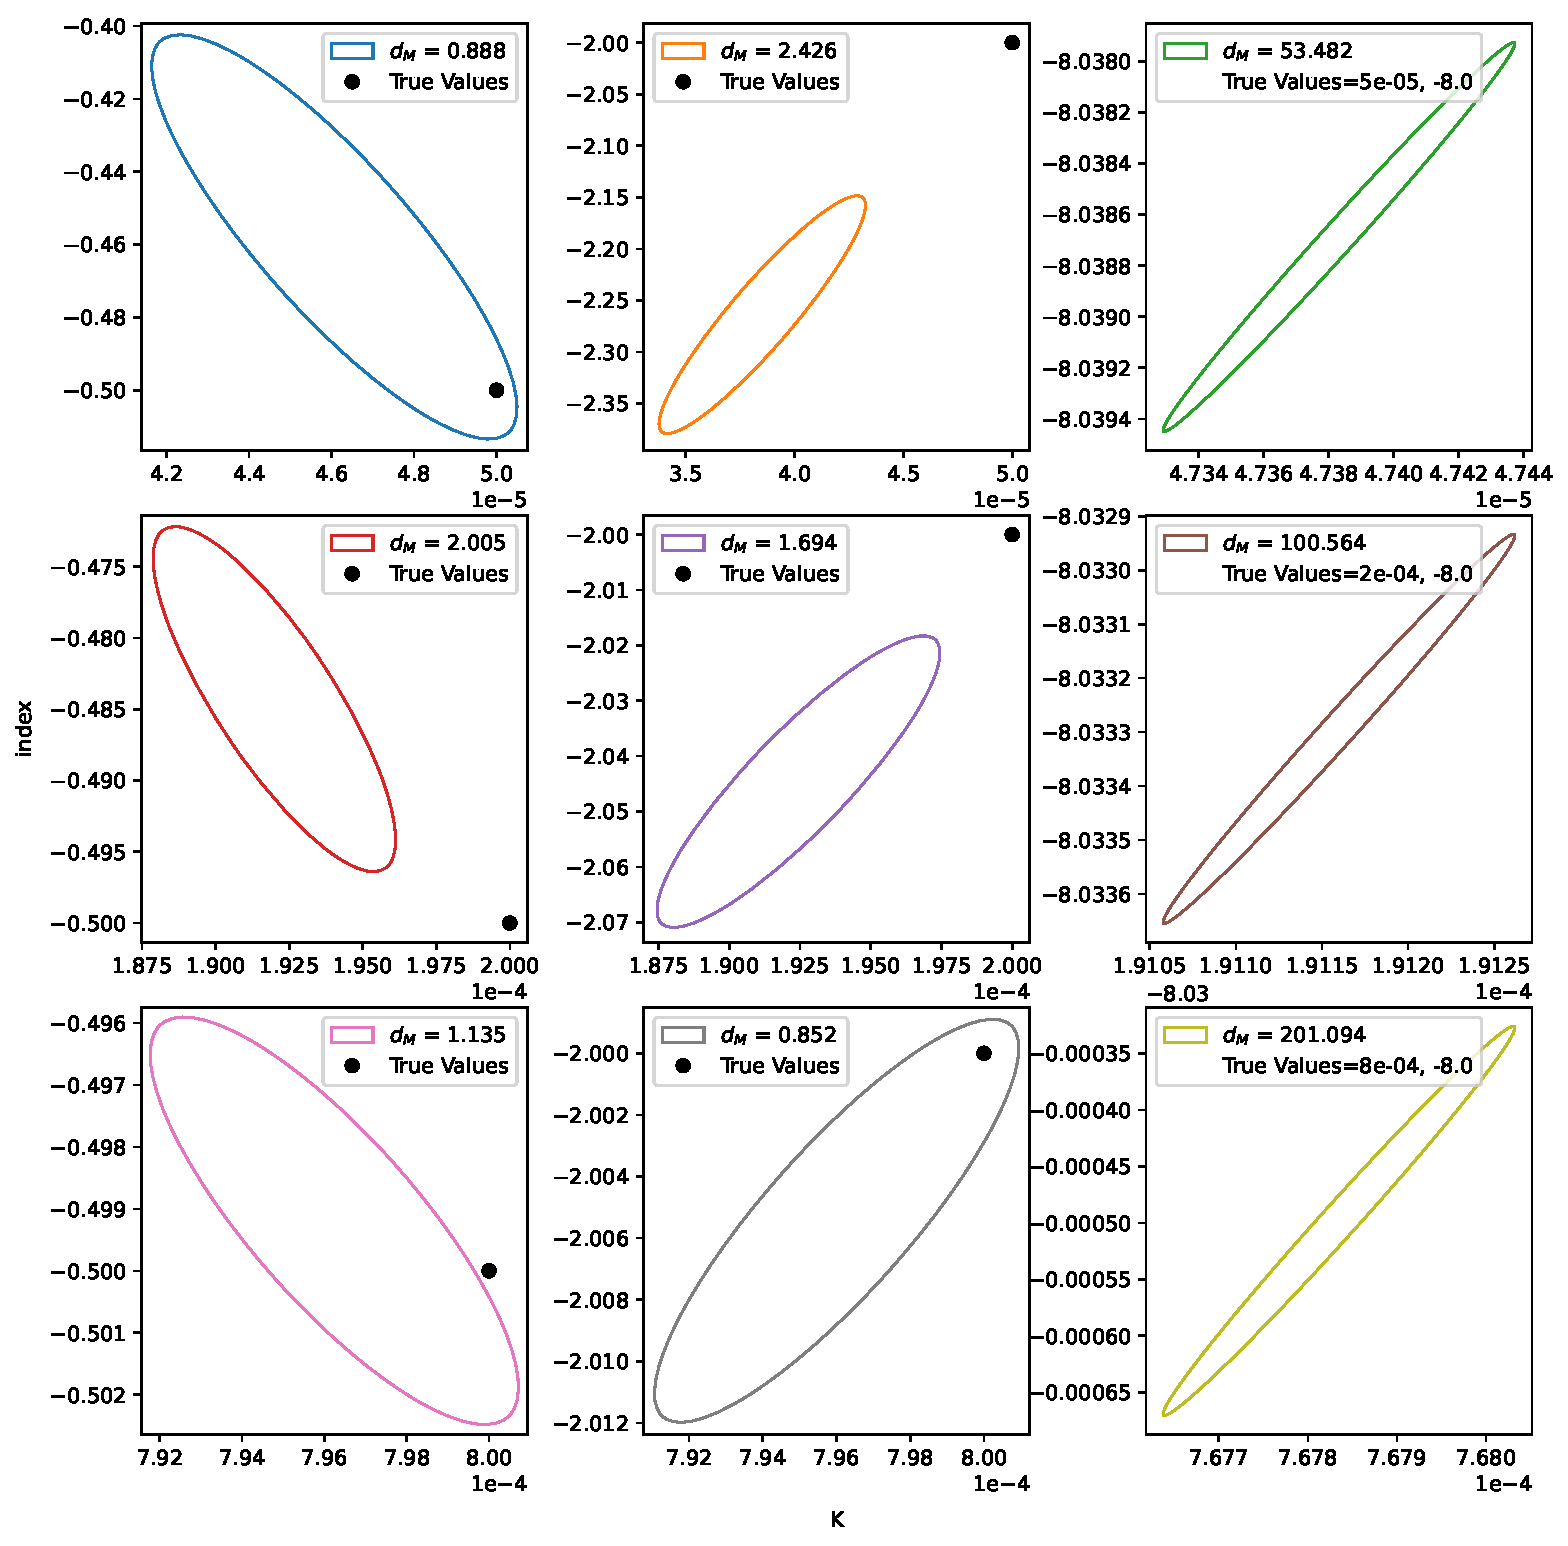
\includegraphics[width=\textwidth]{Images/Pure_Simulation/combined_plots_different_sources.pdf}
  \caption{Count spectra with different simulated powerlaw sources fitted. The source luminosity is changed across the different rows and the source index is changed across columns. The pivot value of the powerlaws used is at $piv=100$keV, meaning that the central plot of the bottom row shows a Crab-like source.}
  \label{fig diff powerlaws}
\end{figure}

Another important test is changing the index and normalization of the simulated source and measuring the effect on the fit quality.  According to figure \ref{fig diff powerlaws}, the posterior uncertainties increase for dimmer sources but the accuracy is unchanged as expected. 

The exception to this are steep powerlaws with $index=-8$, for which the fit presents large systematic errors. This behavior is caused by the SPI response matrix. Increasing the number of energy bins for both the model energy bins and the number of SPI-data energy bins causes the error to disappear, as shown in figure \ref{fig large index}. The original SPI response functions are measured at 51 different energies across SPIs wide energy range from 20keV to 8MeV. PySPI then interpolates these original response functions to suitably match both model and data energy bins of choice. For the time being it is unclear whether the systematic error at large indices is a result of an error in the interpolation algorithm of the PySPI response functions, or simply a result of having to do the interpolation in the first place. Regardless, the error does not occur at source spectra with smaller indices, like the Crab Nebula with $index\approx-2$. Furthermore, the error can easily be avoided by using larger response matrices whenever large indices need to be fitted.





\subsection{Second Source}

\begin{figure}[h]
  \centering
  \makebox[\textwidth][c]{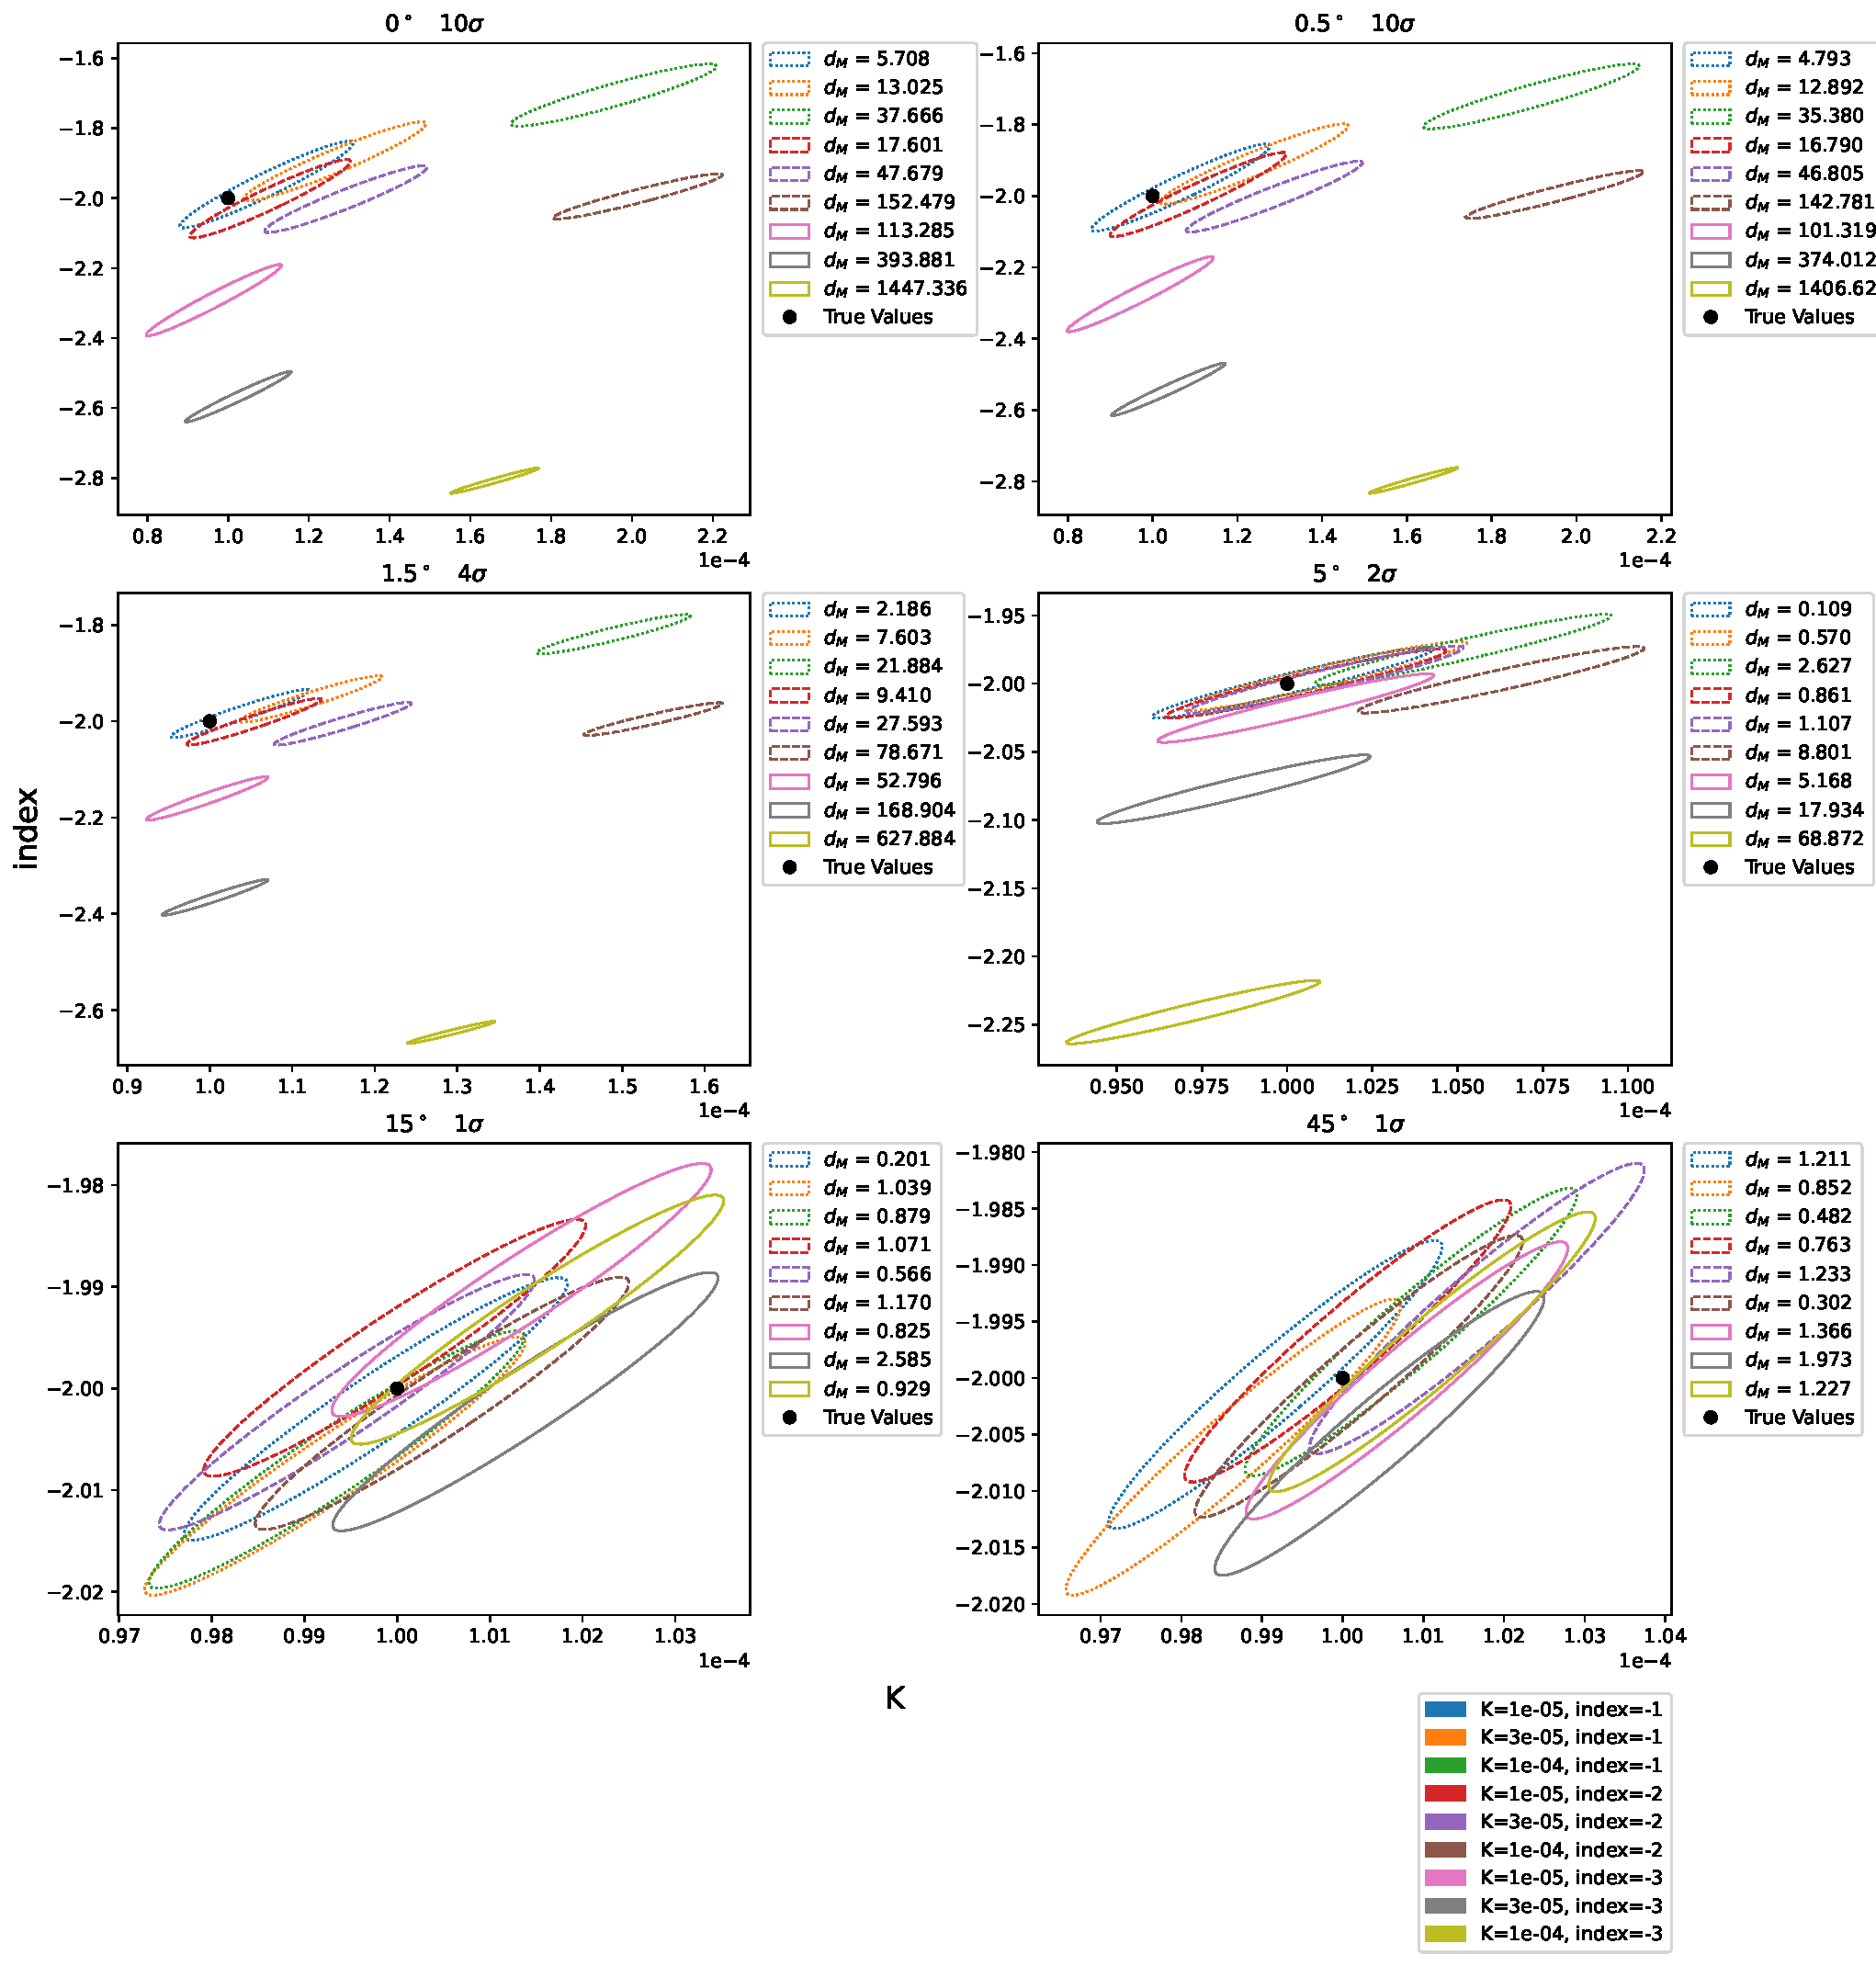
\includegraphics[width=1.1\textwidth]{Images/Pure_Simulation/combined_plots_second_source.pdf}}%
  \caption{The effects of a second source, which is not included in the source model of the fit, on the quality of the fit for the primary source. The different plots show results for different angular distances between the two sources, as stated in the respective titles. The titles further show the amount of standard deviations illustrated by the ellipses. Finally, see the legend at the bottom right for the powerlaw parameters of the second source. All powerlaws are normalized at $piv=200$keV.}
  \label{fig sec source}
\end{figure}

In practical applications there are almost always going to be additional sources within SPI's field of view that are not considered in the source model. This invalidates the assumption that background count rates are constant in corresponding bins within clusters. In order to judge the severity of this, we shall simulate a second source within SPI's field of view (not included in the source model) to observe to ramifications of the fit on the primary source, as is shown in figure \ref{fig sec source}. 

When the two sources are close to each other, the normalization and index shift in accordance to the second source as expected. At 5 degrees apart most fits start to achieve a decent level of quality, and at 15 degrees or more the impact is negligible. The impact is largest when the second source has a large (on an absolute scale) index. We conclude that it is very important to include all sources within $5^\circ$ the primary source.

\FloatBarrier

\begin{figure}[h]
  \centering
  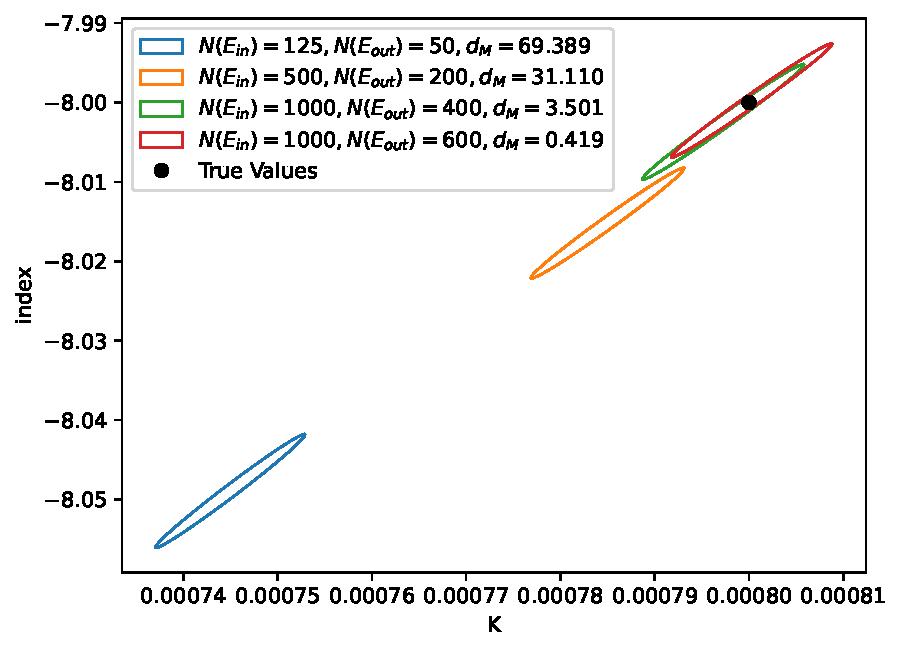
\includegraphics[width=0.6\textwidth]{Images/Pure_Simulation/large_index_combined_plot_10sig.pdf}
  \caption{Powerlaw with $index=-8$ fitted using response matrices of different sizes. $N(E_{in})$ describes the number of energy bins used to describe the source model and $N(E_{out})$ the number of energy bins used for the SPI counts. The confidence interval ellipses show 10 standard deviations each.}
  \label{fig large index}
\end{figure}

\subsection{Data Scaling}



\begin{figure}[H]
  \centering
  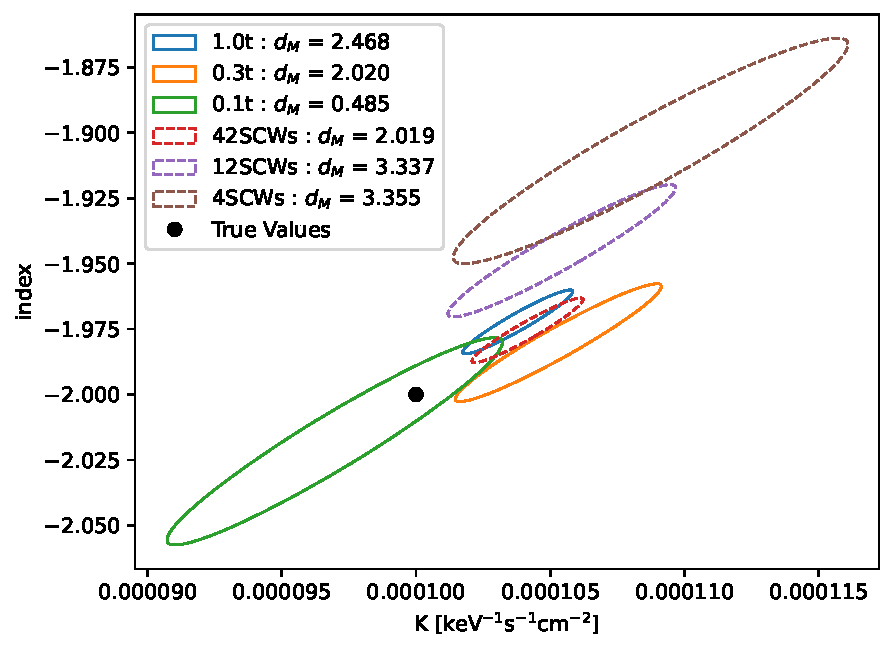
\includegraphics[width=0.6\textwidth]{Images/Pure_Simulation/combined_plots_data_scaling.pdf}
  \caption{Fit results from scaling the amount of lifetime $t$ in each SCW or the amount of SCWs used.}
  \label{fig data scaling}
\end{figure}

Generally speaking, more data will produce better results in any fit. We can test the scaling behavior of the fit quality with the amount of data available to PySpi by scaling the amount of lifetime in each SCW and by scaling the amount of SCWs used in the fit, as shown in figure \ref{fig data scaling}. Unsurprisingly, the fit quality scales very similarly with both of these parameters. The scaling further implies that even larger datasets will produce even smaller uncertainties and errors in the fit. 


\subsection{Angular Distance between SCWs}

\begin{figure}[h]
  \centering
  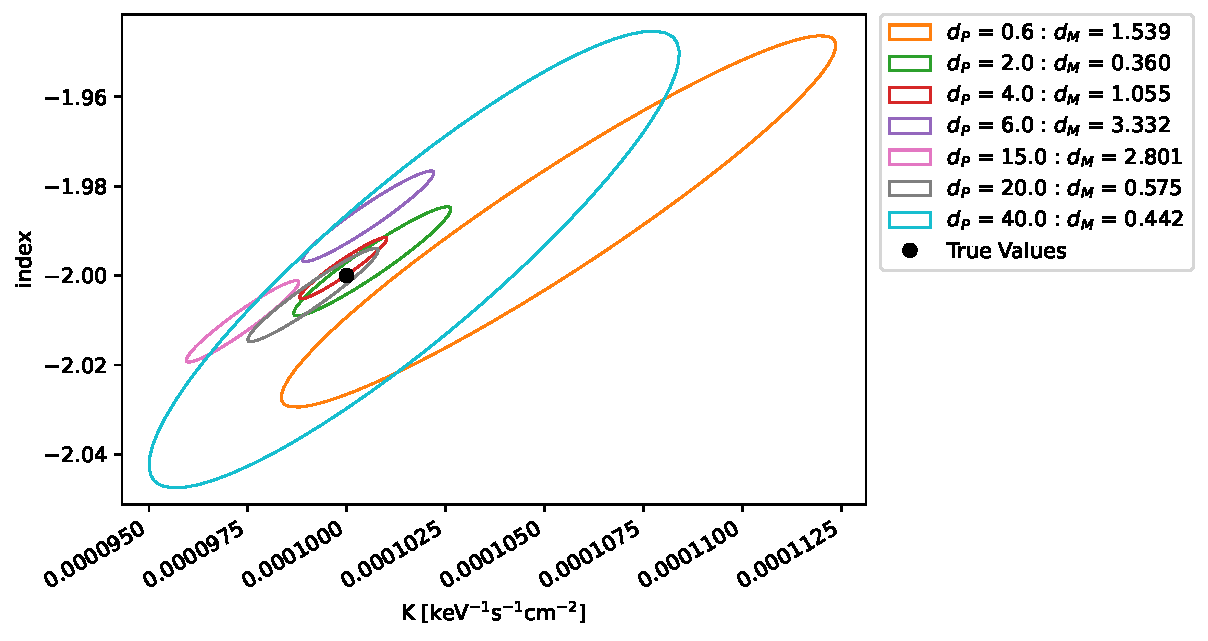
\includegraphics[width=0.8\textwidth]{Images/Pure_Simulation/combined_plot_pointing_distances.pdf}
  \caption{Fit results for two SCWs with different angular distances $d_p$ (in degrees) between them. The center between the two SCWs is always orientated directly towards the source.}
  \label{fig pointing distances}
\end{figure}

A very important parameter when conducting these fits is knowing the optimal angular distance between SCWs in clusters, as shown in figure \ref{fig pointing distances}. Pointings with distances between 2 and 20 degrees all produced good results. Any angular distance outside of those values should be avoided. The very best result (with the smallest uncertainty) was attained for an angular distance of 4$^\circ$.

For this simulation and the next one the count spectrum was not simulated using the SCWs of revolution 0374 as a baseline, since custom orientations are required. Instead one cluster of 2 SCWs with custom orientations are used.


\subsection{Angular Distance between Source and Cluster}

\begin{figure}[H]
  \centering
  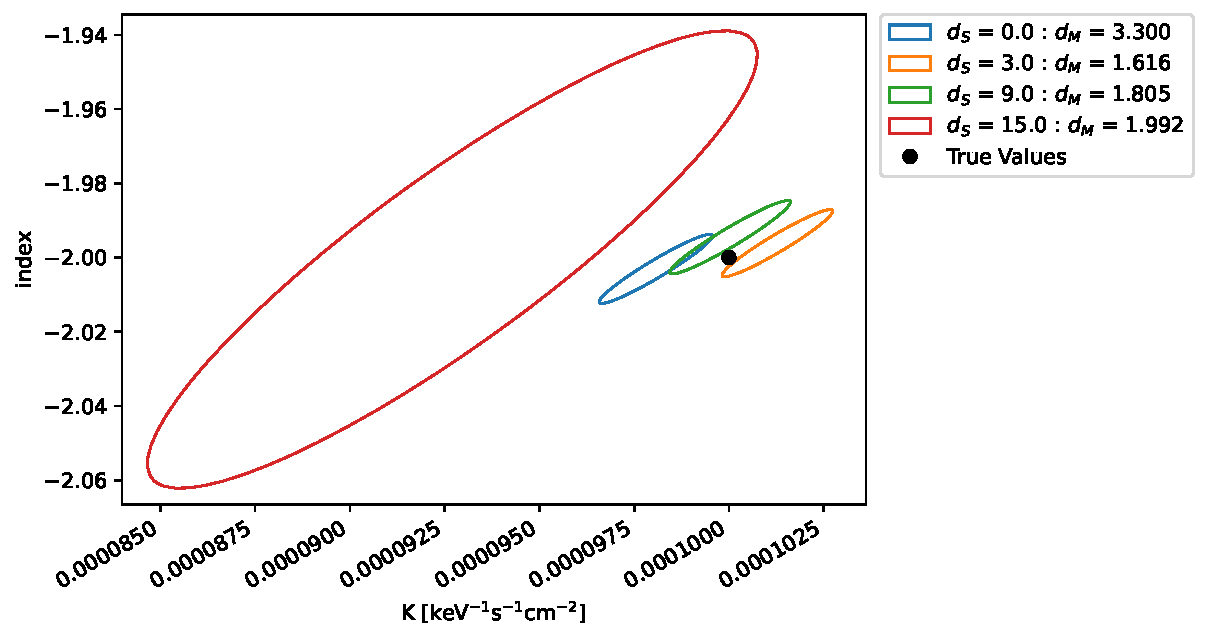
\includegraphics[width=0.9\textwidth]{Images/Pure_Simulation/combined_plot_source_distances.pdf}
  \caption{Two SCWs with an angular distance of $4^\circ$ between them are clustered, and then rotated so that the center between them is $d_S$ degrees away from the source. The fit results for different distances are shown.}
  \label{fig source distance}
\end{figure}

A similar yet equally important parameter for the SCW clustering algorithm is the maximum angular distance between pointings and the source. This is explored in figure \ref{fig source distance}. Anything within 9 degrees of the source provides equally good results, but as the distance approaches the edge SPIs $16^\circ$ field of view, the fit precision drastically worsens. 

\FloatBarrier


\subsection{Cluster Size}

\begin{figure}[h]
  \centering
  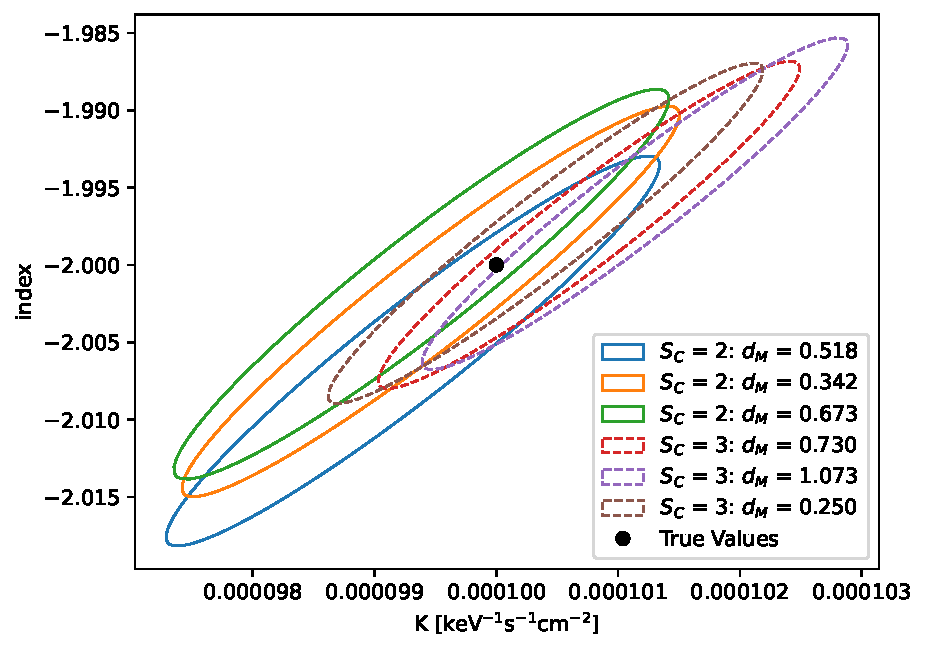
\includegraphics[width=0.7\textwidth]{Images/Pure_Simulation/combined_plots_cluster_size.pdf}
  \caption{The same dataset fitted repeatedly using clusters sizes $S_C$ of two and three.}
  \label{fig cluster size}
\end{figure}

So far we have only been using SCW clusters of size two ($S_C=2$) in the fits. Figure \ref{fig cluster size} compares fits using cluster size $S_C=2$ to $S_C=3$. Although the difference is not large, we do see a consistent improvement in the the uncertainty size of the fit parameters. Even larger clusters may accentuate this improvement even further. However, in practical applications larger cluster sizes also have downsides. For one, calculating the maximum likelihood background value becomes more complex, and secondly, the the assumption of a constant background count-rate within SCW clusters may become harder to fulfill, since larger cluster sizes necessarily mean larger temporal and spatial differences in the SCWs of the clusters.


\subsection{Fitting the Source Position}

\begin{figure}[h]
  \centering
  \makebox[\textwidth][c]{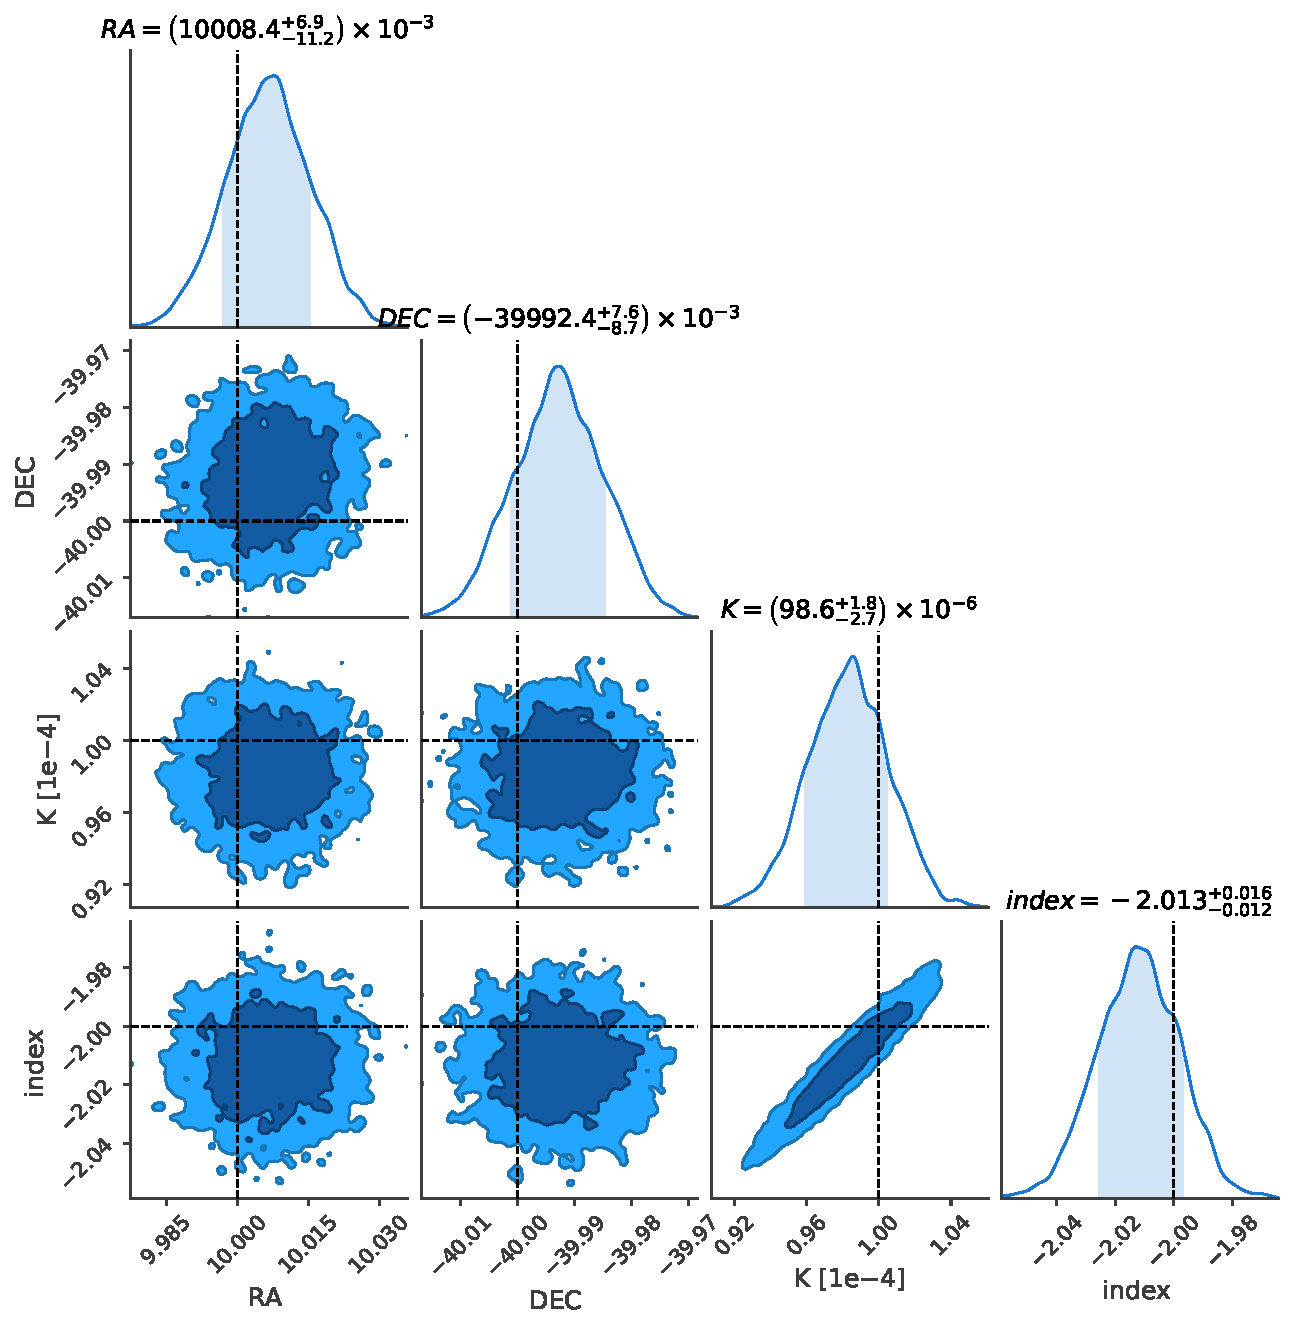
\includegraphics[width=1.1\textwidth]{Images/Pure_Simulation/source_position.pdf}}%
  \caption{The posterior parameter distribution when fitting the source position along with spectral parameters. The dashed black lines indicate the true values. As always, the flux normalization $K$ is measured in keV$^{-1}$s$^{-1}$cm$^{-2}$.}
  \label{fig pos fit}
\end{figure}

Naturally we are not restricted to fitting spectral parameters of sources. The source position, for example, can also be included as parameters in the fit. The resulting posterior distributions of such a fit are shown in figure \ref{fig pos fit}. The results show a high degree of accuracy and precision, with all parameters within one standard deviation of the true values.


\section{Mixed Simulation and Spimodfit Comparison} \label{sec: smf comparison}




Having tested how well the PySPI fitting procedure works for purely simulated data where we know that the fundamental assumption of constant background rates is fulfilled, we may now move on to test how well the fit performs on mixed simulations, where the background counts are entirely real but the source spectrum remains simulated. This allows us to get a better understanding of how well the method works for realistic conditions but retain the advantage of knowing the true source model parameters in every fit. Additionally, this dataset is suitable to be fitted using Spimodfit due to it using real background counts, which the spimodfit background model is designed for. The procedure for using Spimodfit is described in appendix \ref{smf procedure}.

Before any fits can be conducted, a count spectrum needs to be created first. This can be done in almost the exact same steps as the purely simulated count spectrum form section \ref{sec: pure sim}, except step \ref{step pure sim back}, where we duplicate the counts from one SCW onto all other SCWs, is skipped entirely. This way the entire count spectrum from this revolution is used as background, and the simulated source counts are added on-top. Naturally, the choice of revolution is much more important here, since any sources in SPIs field of view will not be considered in the source model and hence invalidate the assumption of constant background rates within clusters. Revolution 0374 is used for this purpose, as it allows us to place our simulated source at the equatorial coordinates $RA=10^\circ, DEC=-40^\circ$, where no bright sources exist within SPIs field of view.

When fitting data using Spimodfit, a background model is created. This background model can be accessed (see section \ref{spimodfit bkg}) and provides us with another option for generating a count spectrum, as the simulated source counts can be added to the background counts from the spimodfit model.

\begin{figure}[h]
  \centering
  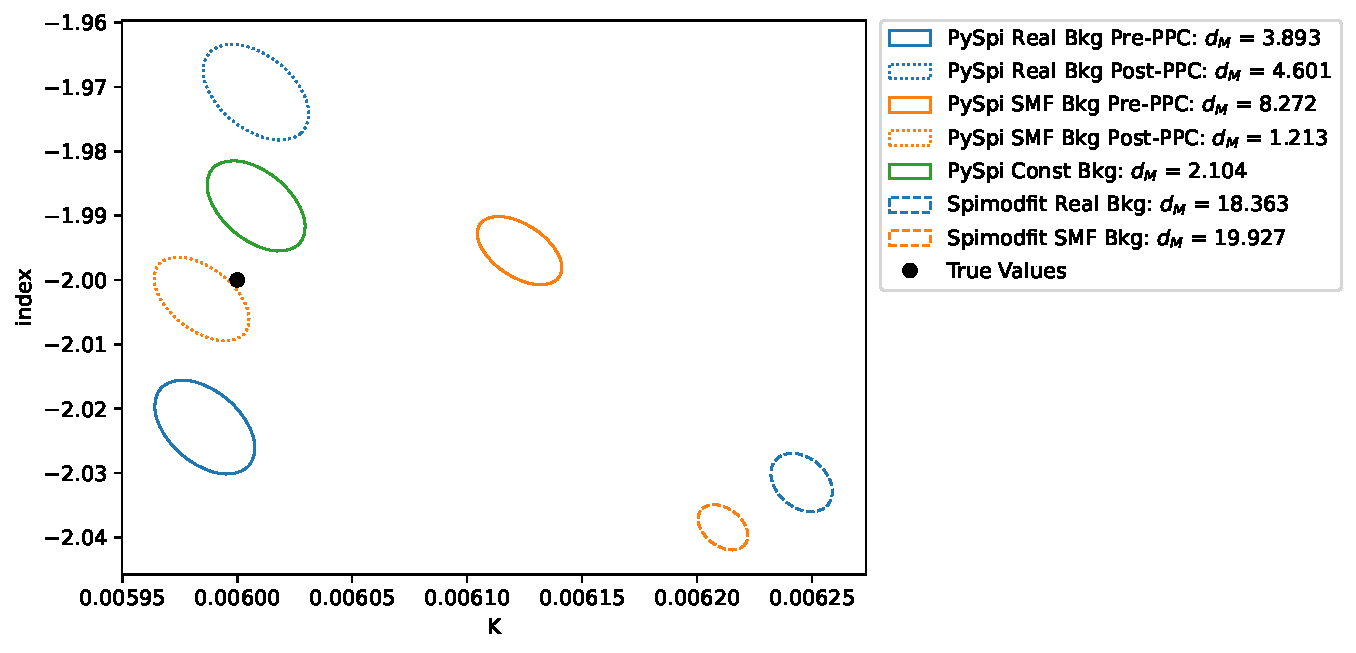
\includegraphics[width=0.9\textwidth]{Images/SMF_Comparison/spimodfit_comparison_combined_plot.pdf}
  \caption{Fit results of the mixed simulation count spectra when fitted using PySPI and Spimodfit. }
  \label{fig smf comparison}
\end{figure}

Both of these count spectra (real background counts and spimodfit background model counts) were fitted using PySPI and Spimodfit, the results of which are illustrated in figure \ref{fig smf comparison}. For further comparison purposes, a PySPI fit using the constant background counts (exactly as in section \ref{sec: pure sim}) is also shown. The PySPI fits all perform comparably well. The real background fit is the largest number of standard deviations from the true values, but this could just as well be a statistical fluctuation. Interestingly, the Spimodfit fits deliver consistently worse results, being almost 20 standard deviations away from the true values. The Spimodfit fit using the Spimodfit background model as background counts in the data spectrum seems to make little difference in the fit quality. One would expect Spimodfit to do very well here, since its background model matches the background in the data perfectly. Despite Spimodfit being considerably less accurate, its result is more precise than the corresponding PySPI fit, delivering uncertainties on its model parameters up to nearly 50\% smaller. 

All of these fits use an energy range of 30-81.5keV. The Spimodfit background model in particular is known to perform worse below 30keV, and it is possible that the SPI response function is not as accurate at the very edge of its energy range as well.


It is worth noting that even when PySPI and Spimodfit use the same revolutions in a fit, the individual SCWs selected to perform the fit may vary. Both methods have independent algorithms for determining suitable SCWs, especially since PySPI has to group the SCWs into appropriate clusters. Spimodfit has its own set of selection criteria to filter out bad SCWs, whereas PySPI relies on PPC analysis (see section \ref{sec:PPC Back}) to remove bad SCW clusters. 


\section{Posterior Predictive Check (PPC) and Background Analysis} \label{sec:PPC Back}
Unusual solar activity, sources not included in the source model, and activation of satellite material from cosmic particles are just a few of the long list of causes may lead to errors in fit of SPI data. This is why Posterior Predictive Checks (PPCs) are a vitally important tool to analyze how well the results of fit actually match the data.

\subsection{PPCs: Theory}

\subsubsection{General Procedure} \label{PPC general}

A PPC is usually conducted in the following way:

\begin{enumerate}
    \item Fit the data to some model, so that a distribution for the posterior is produced.
    \item \label{Posterior sample} Randomly sample from the posterior.
    \item \label{ppc calc count rates} Using the IRF and the model described by the sampled posterior parameters, calculate the expected count rates in every energy bin of every detector of every SCW.
    \item \label{ppc poisson sample} Taking into consideration the lifetime of each detector in every SCW, draw a sample from the Poisson distribution that describes the measured counts in each bin.
    \item Repeat from step \ref{Posterior sample} until a sufficiently detailed distribution of expected counts for every bin is achieved.
\end{enumerate}

This PPC count distribution can then be used in a variety of ways, such as simply plotting the distribution of expected counts next the actually measured counts. One very useful application is the Cumulative Distribution Function (CDF), where one sorts the PPC count distribution of each bin according to size, and then finds the percentile in which the number of actually measured counts falls. If the model described using the posterior values perfectly matches reality one would expect values evenly distributed between 0 and 1, whereas if the model is not a good representation of reality the distribution will not be even. 

In the context of PySPI it makes sense to organize these CDF values into a histogram for every SCW used in the fit. This way individual SCWs for which the model does not match the measured data can be identified and excluded from a repeated fit with hopefully better results. Experience has shown that "bad" SCWs often occur at the beginning or end of INTEGRAL revolutions, which is when SPI approaches its perigee. This places SPI closer to Earth's atmosphere and thus exposes it to a larger number of cosmic-ray air showers, where cosmic-rays interact with particles of the atmosphere and result in a large cascade of interacting particles and sub-particles.

Another useful application for the PPC count distribution is the ability to calculate energy dependant residuals of the source model to the data. To do this one simply takes the sum of the counts in one energy bin over all detectors and all SCWs. This can be repeated for every sample of the posterior predictive counts. The sum of the actually measured counts can then be compared to the distribution of the sums of the posterior predictive counts to determine how many standard deviations the real counts are from the source model for every energy bin. 

\subsubsection{PySPI Application}
There is a problem with using the procedure previously described in section \ref{PPC general} for PySPI: the model used the fit (see section \ref{General Procedure}) is purely a source model, i.e. it tells us nothing about the background count rates. This is a problem because it we cannot calculate the expected count rates in step \ref{ppc calc count rates} of section \ref{PPC general} without being able to describe the background.

The only way to circumvent this problem is with the same approach used in section \ref{General Procedure} of the actual fit. After having calculated the expected source count rates for a sample of the posterior we can use the actually measured counts to calculate the maximum likelihood background count rates and continue our analysis with it.

However, there is a drawback to this solution: in step \ref{ppc poisson sample} of section \ref{PPC general} we can no longer use a simple Poisson distribution to sample expected measured counts from the calculated count rates. This is because we have introduced a bias into our expected count rates by using the actually measured counts in the calculation. For example, if some energy bin has measured a statistically large number of counts (in accordance to the Poisson distribution of the true count rates), then the maximum likelihood background calculated using the actually measured counts will naturally increase with the actually measured counts. This way any statistical outliers are significantly dampened, thus defeating the purpose of conducting the PPC analysis to begin with.

Let us quantify this bias mathematically. The following equations are applicable to every energy bin in every detector in every SCW cluster. As in section \ref{General Procedure} we will focus on clusters of size 2, although the process is analogous for larger cluster sizes.

For every bin in every SCW cluster there exist the true source count rates $s_1$ and $s_2$ as well as a true background count rate $b$. The source count rates vary between the SCWs of one cluster, whereas the background count rate is constant. If $t_1$ and $t_2$ are the lifetimes of the SCWs, the actually measured counts $B_{1m}, B_{2m}, S_{1m}$ and $S_{2m}$ from the respective sources will be Poisson distributed

\begin{align} \label{eq measured counts}
    B_{1m} &\sim \text{Pois}(bt_1) \\
    B_{2m} &\sim \text{Pois}(bt_2) \\
    S_{1m} &\sim \text{Pois}(s_1t_1) \\
    S_{2m} &\sim \text{Pois}(s_2t_2)
\end{align}

so that the total number of measured counts $C_{1m}$ and $C_{2m}$ are simply

\begin{align} \label{eq tot counts ppc}
    C_{1m} &= B_{1m} + S_{1m} \\
    C_{2m} &= B_{2m} + S_{2m}.
\end{align}

Arriving at an equation for the distributions $C_{1m}$ and $C_{2m}$ is our goal for the PPC analysis. We may assume that true source count rates $s_1$ and $s_2$ equal those predicted by our source model from the posterior samples, since testing that assumption is the whole point of doing the PPC analysis to begin with. The true background count rate $b$, however, remains unknown to us. Instead we can only calculate the maximum likelihood background $b_M$, as described previously. In order to be able to draw samples from the probability distributions $C_{1m}$ and $C_{2m}$ we must relate relate the distributions of the quantities that we do know ($s_1, s_2, t_1, t_2, b_M$) to those that we wish to know ($C_{1m}, C_{2m}$ and therefore $B_{1m}, B_{2m}, S_{1m}, S_{2m}$):

\begin{align} \label{eq ppc dif}
    B_{d1} &= B_{1m} - b_Mt_1 \\
    B_{d2} &= B_{2m} - b_Mt_2 \\
    S_{d1} &= S_{1m} - s_1t_1 \\
    S_{d2} &= S_{2m} - s_2t_2.
\end{align}

$B_{d1}$ and $B_{d2}$ tell us the difference between quantities we have readily available ($b_Mt_1$ and $b_Mt_2$) to those directly necessary in the PPC analysis ($B_{1m}$ and $B_{2m}$). This means that if we calculate their variances and approximate the resulting distribution as normal we can directly draw random samples according to the distribution of $B_{1m}$ and $B_{2m}$, without having to know the true background rate $b$. Furthermore, we also have to consider that the distribution of $b_M$, which we utilize in $B_{d1}$ and $B_{d2}$, is correlated with the distribution $S_{1m}$ and $S_{2m}$. Hence, we not only have to calculate the variances of $B_{d1}$ and $B_{d2}$, but also the covariances of $B_{d1}$ with $S_{d1}$ and $B_{d2}$ with $S_{d2}$, respectively. To draw a random sample from $B_{1m}$, $S_{1m}$, $B_{2m}$ and $S_{2m}$ we thus sample from a multivariate normal with mean $\mu$ and covariance matrix $cov$:

\begin{align}
    \mu_1 &= \begin{pmatrix}
        b_Mt_1 \\ s_1t_1
    \end{pmatrix} \\
    \mu_2 &= \begin{pmatrix}
      b_Mt_2 \\ s_2t_2
  \end{pmatrix} 
\end{align}
\begin{align} \label{eq: covs mats}
    cov_1 &= \begin{bmatrix}
        \text{variance}(B_{d1}) & \text{covariance}(B_{d1}, S_{d1})\\ \text{covariance}(B_{d1}, S_{d1}) & \text{variance}(S_{d1})
    \end{bmatrix} \\
    cov_2 &= \begin{bmatrix}
      \text{variance}(B_{d2}) & \text{covariance}(B_{d2}, S_{d2})\\ \text{covariance}(B_{d2}, S_{d2}) & \text{variance}(S_{d2})
  \end{bmatrix}
\end{align}
Hence: 
\begin{align} \label{eq mult var norm ppc}
    \begin{pmatrix}
        B_{1m} \\ S_{1m}
    \end{pmatrix}
    &\sim \mathcal{N}(\mu_1, cov_1)\\
    \begin{pmatrix}
      B_{2m} \\ S_{2m}
  \end{pmatrix}
  &\sim \mathcal{N}(\mu_2, cov_2)
\end{align}
This works because the expected value of the maximum likelihood background rate is equal to the true background rate: $E(b_M) = b$. It is worth noting that approximating the distribution shapes as normal should have negligible impact as long as the number of counts per bin are sufficiently large.

Having understood the motivation, the difficulty lies in actually calculating these variances. Considering the already complicated distribution of the maximum likelihood background (equation \ref{eq: max lik back})

\begin{equation}\label{eq max lik back 2}
  b_M = \frac{1}{2} \left[ \frac{C_t}{t_t} - s_t + \sqrt{\left( \frac{C_t}{t_t} - s_t\right)^2 + 4 \left( \frac{C_1s_2+C_2s_1}{t_t}-s_1s_2\right)}\right]
\end{equation}

where $C_1$ and $C_2$ are Poisson distributions, solving for the covariance matrices $cov_1$ and $cov_2$ analytically seems nearly impossible.


\subsection{PPCs: PySPI Implementation}

Fortunately, instead of solving for $cov_1$ and $cov_2$ from equation \ref{eq: covs mats} analytically, it is possible to approximate the result through numerical sampling. Given some background rate $b$, source rates $s_1$ and $s_2$, and lifetimes $t_1$ and $t_2$, we can numerically sample the detected count rates $B_{1m}, S_{1m}, B_{2m}, S_{1m}$ (equations \ref{eq measured counts}), which allows us to calculate the maximum likelihood background $b_M$ (equation \ref{eq max lik back 2}) and therefore $B_{d1},S_{d1},B_{d2}$ and $S_{d2}$ (equations \ref{eq ppc dif}). If we repeat this often enough (e.g. 10000 times) we can thus estimate $cov_1$ and $cov_2$ (equations \ref{eq: covs mats}). Since $E(b_M) = b$ it is irrelevant that we don't know $b$ and we can use $cov_1$ and $cov_2$ sampled using $b_M$ instead. Finally we make use of equations \ref{eq mult var norm ppc} and \ref{eq tot counts ppc} to be able to sample $C_{1m}$ and $C_{2m}$, as was our goal.

One issue with this approach is that the sample covariance matrix is only true at the input parameters ($b_M,s_1,s_2,t_1,t_2$) used to sample it. Although taking 10000 samples to estimate the matrix doesn't take long, it definitely takes too long to do so for every combination of input parameters encountered in a typical SPI fit. The solution is to find the minimum and maximum of each of the five input parameters encountered in the data after a fit, estimate the covariance via sampling at a grid covering values between the minimum and maximum for each of the input parameters, and then interpolating the matrix along the grid for any possible input combination encountered. 

\begin{figure}[h]
  \centering
  \makebox[\textwidth][c]{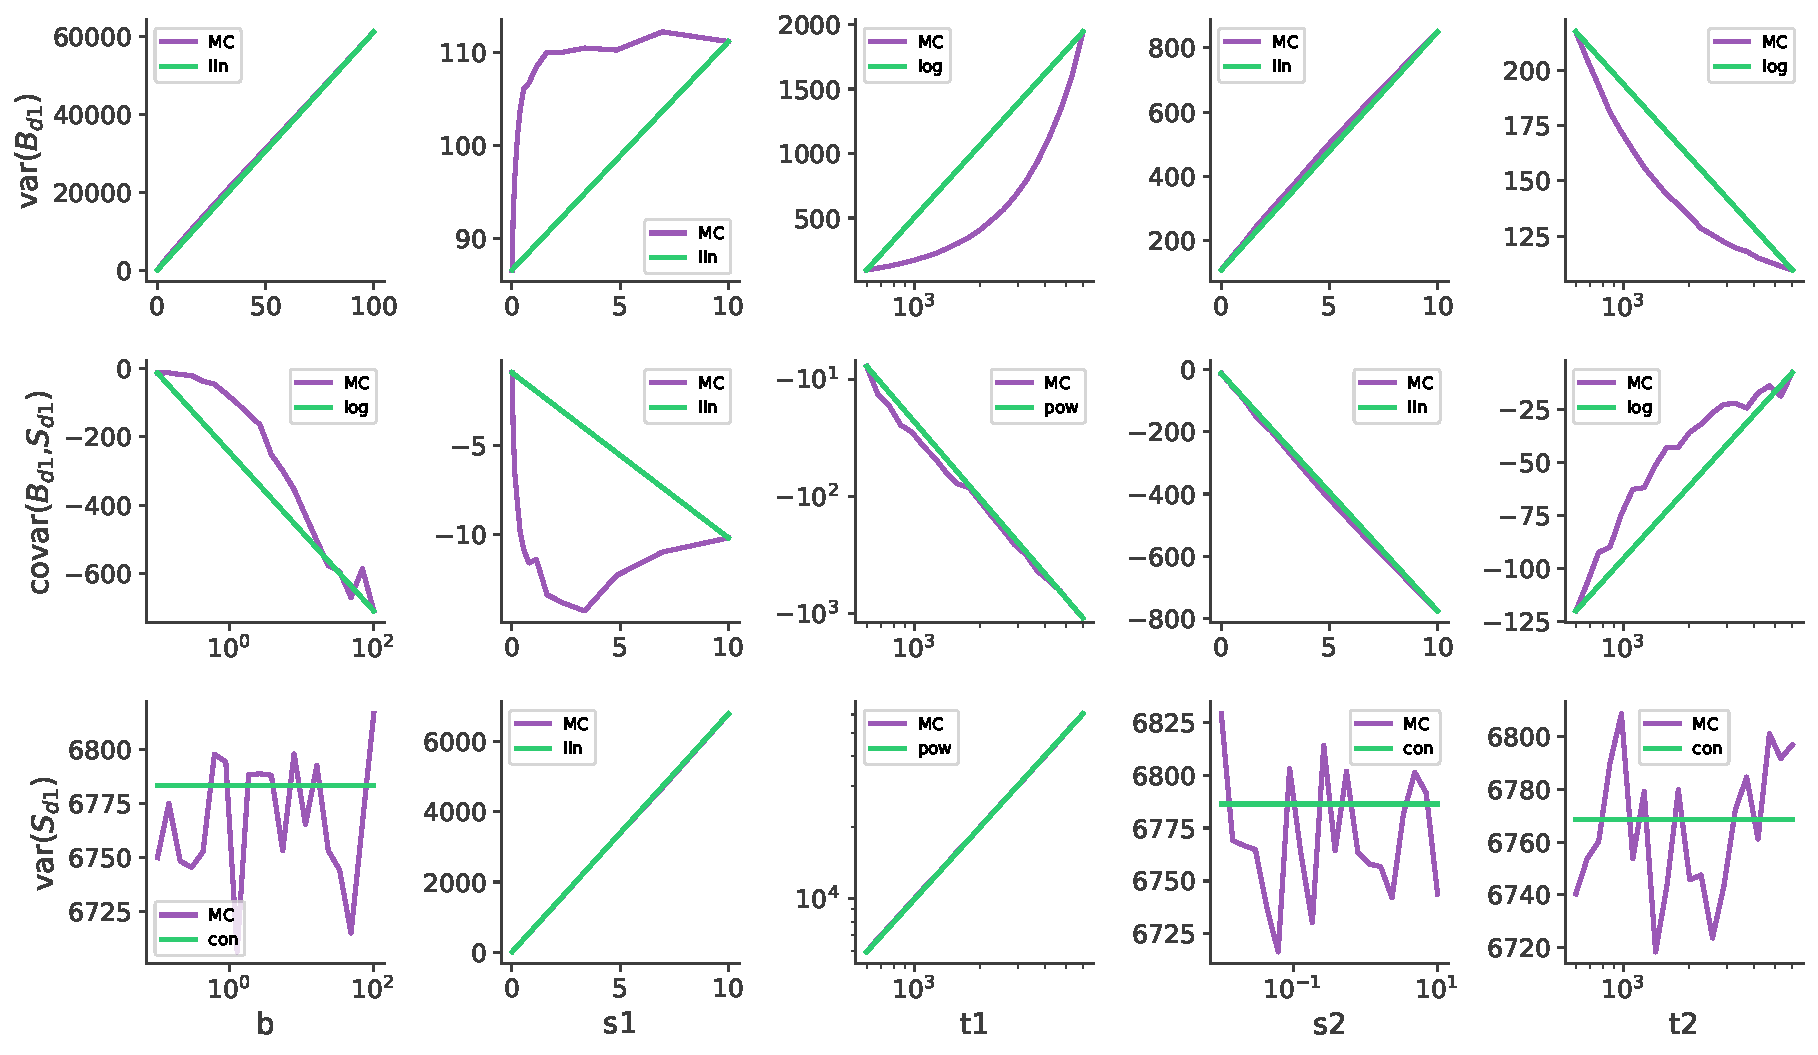
\includegraphics[width=1.05\textwidth]{Images/PPC_and_Background_Analysis/PPC_scaling_different_1_bright_short.pdf}}%
  \caption{The scaling behavior of elements of the covariance matrix $cov_1$ as a function of its input parameters over select intervals (purple). In green we see how different interpolation functions (constant, linear, logarithmic, powerlaw) could be used in an attempt to match the scaling behavior by interpolating from the first to the last data-point. }
  \label{fig ppc scaling}
\end{figure}

Figure \ref{fig ppc scaling} shows how elements of the covariance matrix scale when the different input parameters are changed. Note that the scaling behavior changes quite significantly depending on where in the input parameters space one looks, so figure \ref{fig ppc scaling} is not representative for all input ranges. Initially the plan was to approximate the scaling of each matrix element and input parameter pair through a different scaling function. However, this has been found to lead to numerical instabilities, so linear scaling was implemented across the board.

For a typical SPI fit of a Crab-like source with logarithmically spaced energy bins $b_M$ will usually vary within two orders of magnitude, $s_1$ and $s_2$ will vary between three orders of magnitude, and $t_1$ and $t_2$ will stay within one order of magnitude. It has been found that using 9 grid values along the $b_M$ axis, 12 grid values along the $s_1$ and $s_2$ axes, and 5 grid values along the $t_1$ and $t_2$ axes (all spaced logarithmically) are sufficient to accurately interpolate the covariance matrix for all possible input parameters. This means that the covariance matrix is independently sampled (using 10000 samples each) at $9\cdot12^2\cdot5^2=32400$ different input combinations. For each input combination encountered after the fit in the PPC analysis, the closest $2^5=32$ grid points are selected and interpolated to reach a final covariance matrix, which is then used to sample the measured counts using the multivariate normal distribution. 

There are many ways to further numerically optimize this procedure, such as taking advantage of the inherent symmetry in the interpolation matrix from both detectors or using more accurate scaling behavior in the interpolation functions, but since the actual PySPI fits still take much longer than the PPC covariance computation this has been left as a project for the future.


\subsection{PPCs: Results} \label{sec ppc results}

\begin{figure}[h]
  \centering
  \begin{subfigure}{0.5\textwidth}
    \centering
    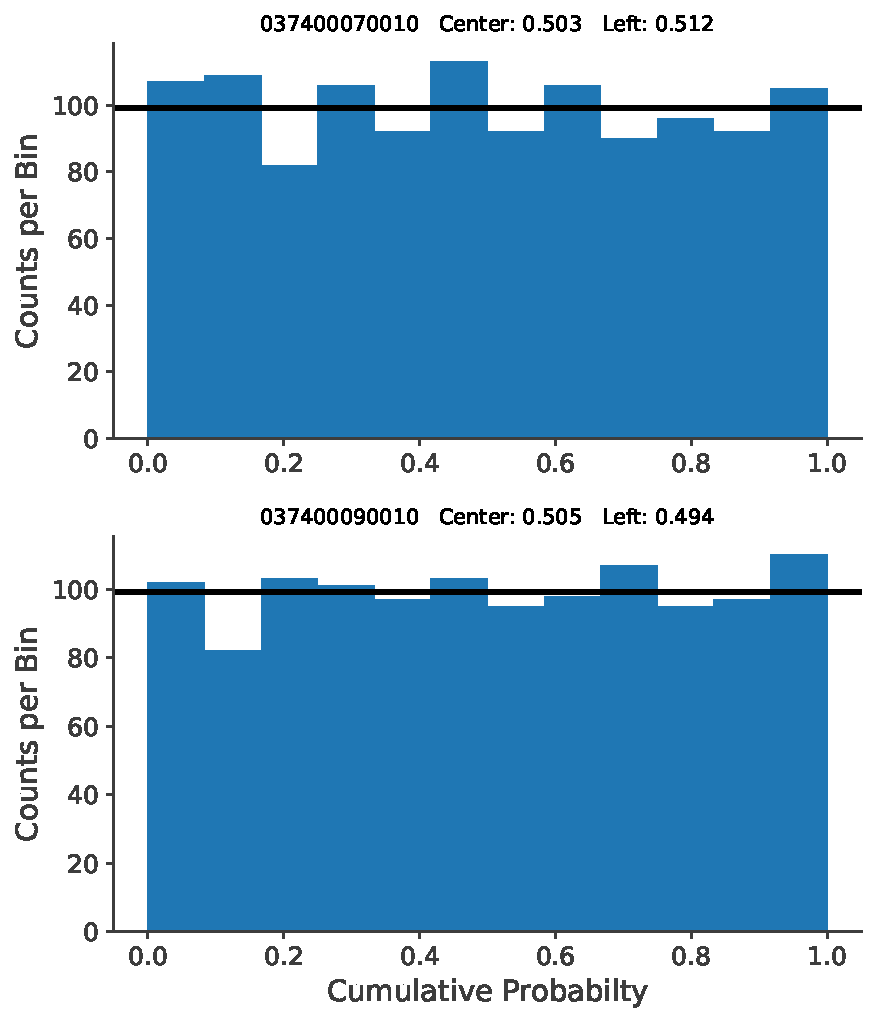
\includegraphics[width=0.9\linewidth]{Images/PPC_and_Background_Analysis/037400070010_037400090010_cdf.pdf}
    %\caption{A subfigure}
    %\label{fig:sub1}
  \end{subfigure}%
  \begin{subfigure}{.5\textwidth}
    \centering
    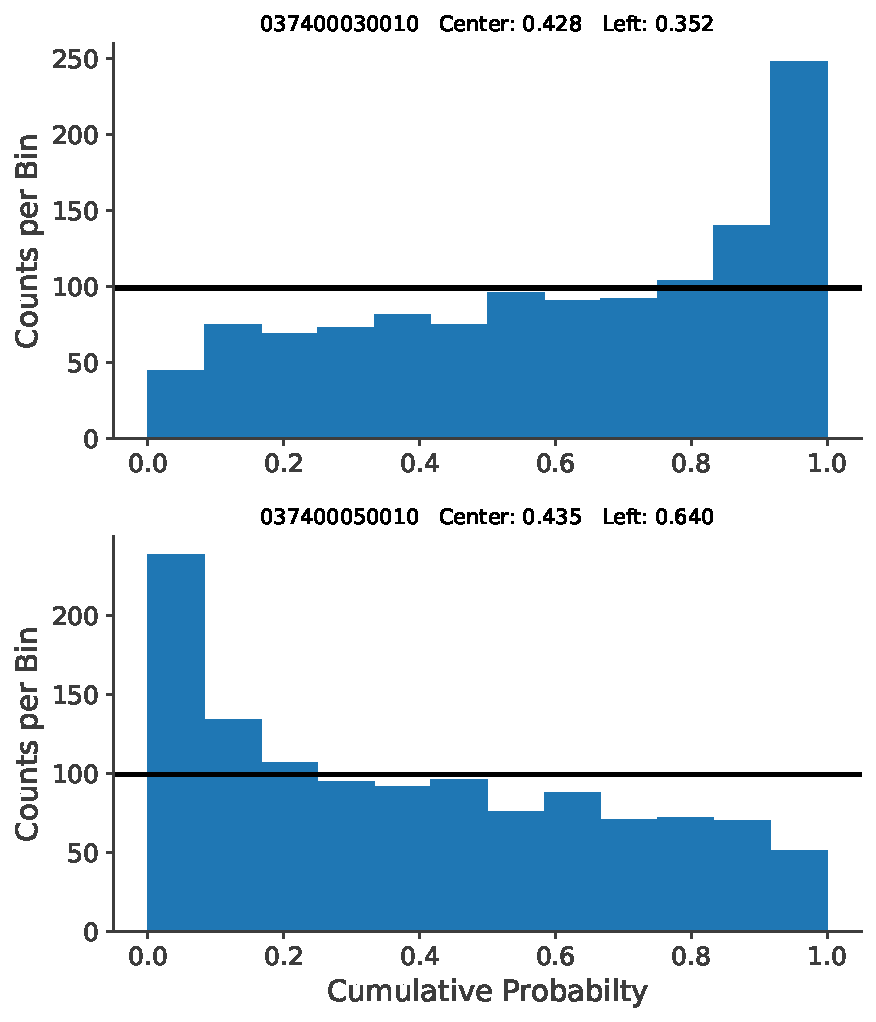
\includegraphics[width=.9\linewidth]{Images/PPC_and_Background_Analysis/037400030010_037400050010_cdf.pdf}
    %\caption{A subfigure}
    %\label{fig:sub2}
  \end{subfigure}
  \caption{Example of a cluster with a "good" CDF distribution (left column) and a cluster with a "bad" CDF distribution (right column).  Since clusters consist of two pointings, the two CDF histograms from each pointing in the clusters are shown in columns. Also shown next to the SCW IDs of the pointings are the proportion of counts on the left half and the central half. The solid black line shows the ideal distribution. Both of these clusters were taken from the same fit.}
  \label{fig ppc cdf ex good and bad}
  \end{figure}



For each cluster in the fit the CDF distribution will be analyzed. This means that the PPC distribution of expected counts based on the posterior distribution of the source model parameters is computed, and then the actual count number of the data is compared to this distribution. The percentile in which the real count data can be sorted into the predicted count distribution is recorded, leading to the CDF distribution when aggregated over all bins. It is worth clarifying that these CDFs are not used in the traditional sense of a monotonously increasing function from from 0 to 1, but that these CDF distributions display the histogram of where every actually measured count falls on the CDF distribution of the PPC sampled counts. If the source model matches the data well then we expect the CDF to be evenly distributed along all percentiles. Example of clusters with "good" and "bad" CDFs are shown in figure \ref{fig ppc cdf ex good and bad}. After having conducted a fit and plotted CDF distributions for all clusters, the "bad" clusters can be identified and removed from the list of clusters. The fit is then executed again using only "good" clusters, yielding (hopefully) improved results. The CDF histograms from all pointings within one cluster are naturally correlated since the maximum likelihood background is calculated using measured counts from all pointings in the cluster. Therefore the CDFs of all pointings within a cluster should be observed together.




To test our newly developed PPC capabilities, we shall use the same count spectrum using real background counts from revolution 0374 and a simulated Crab-like powerlaw that was already used in section \ref{sec: smf comparison}. The data is fit twice: once with SCW clusters with a minimum angular distance between them set to to $1.5^\circ$, and once with $2.5^\circ$ (see appendix \ref{Clustering Algorithm} for more info on the clustering algorithm). Since consecutive SPI pointings are often $2.1^\circ$ apart, this change makes the difference between pairing up consecutive SCWs together (e.g. 03740003 with 03740004, 03740005 with 03740006) and pairing up offset consecutive SCWs together (e.g. 03740003 with 03740005, 03740004 with 03740006). This can be both advantageous and disadvantageous. As shown in figure \ref{fig pointing distances} the optimal angular distance between pointings lies closer to $4.0^\circ$, so using a minimum distance of $2.5^\circ$ should improve fit precision in that regard. However, larger time windows between SCWs increases the probability for background count rates to change, meaning that a minimum distance of $2.5^\circ$ could also decrease fit quality. 

The results of these fits are shown in figures \ref{ppc indv fits 1.5} and \ref{ppc indv fits 2.5}. In these figures we see combined pre-PPC fits, using all SCW clusters, and post-ppc fits, using only SCW clusters with good PPC-CDFs. Also shown are the results of fitting each SCW cluster individually, where those with good CDFs are shown in green and those with bad CDFs are shown in red. 

For a minimum distance of $1.5^\circ$ the fit results of individual clusters seem to largely be statistically distributed. There are no clusters with severely bad CDF distributions, and the one that was identified as a bad cluster does not have a significant impact on the overall fit. This is because the background for consecutive pointings in this revolution stays sufficiently constant (shown in section \ref{sec back anal}), so that a PPC analysis is mostly unnecessary.

However, for a minimum distance of $2.5^\circ$ the background count rates do not stay nearly as constant within clusters (shown in section \ref{sec back anal}), so that conducting a PPC analysis is more constructive. Figure \ref{ppc indv fits 2.5} shows that the clusters with bad CDFs are all at the edge of the distribution from all individual cluster fits.

Based on figures \ref{ppc indv fits 1.5} and \ref{ppc indv fits 2.5} one might think that the post-PPC fits using only clusters with good PPCs does not offer a significant improvement. This is because all SCWs used from 0374 are relatively well behaved, with even the worst cluster (figure \ref{fig ppc cdf ex good and bad}, right) performs decently well. When fitting larger datasets it is not uncommon to encounter clusters with drastically worse results, such as shown in figure \ref{fig ppc really bad total}. Those outliers are significantly more impactful and are absolutely essential to remove when attempting a high quality fit. Figure \ref{fig ppc really bad total} also shows the total CDF across all clusters in a fit. The distribution matches the expected distribution almost perfectly, indicating that the the method for approximating PPC distributions is sufficiently accurate. 

\begin{figure}[H]
  \centering
  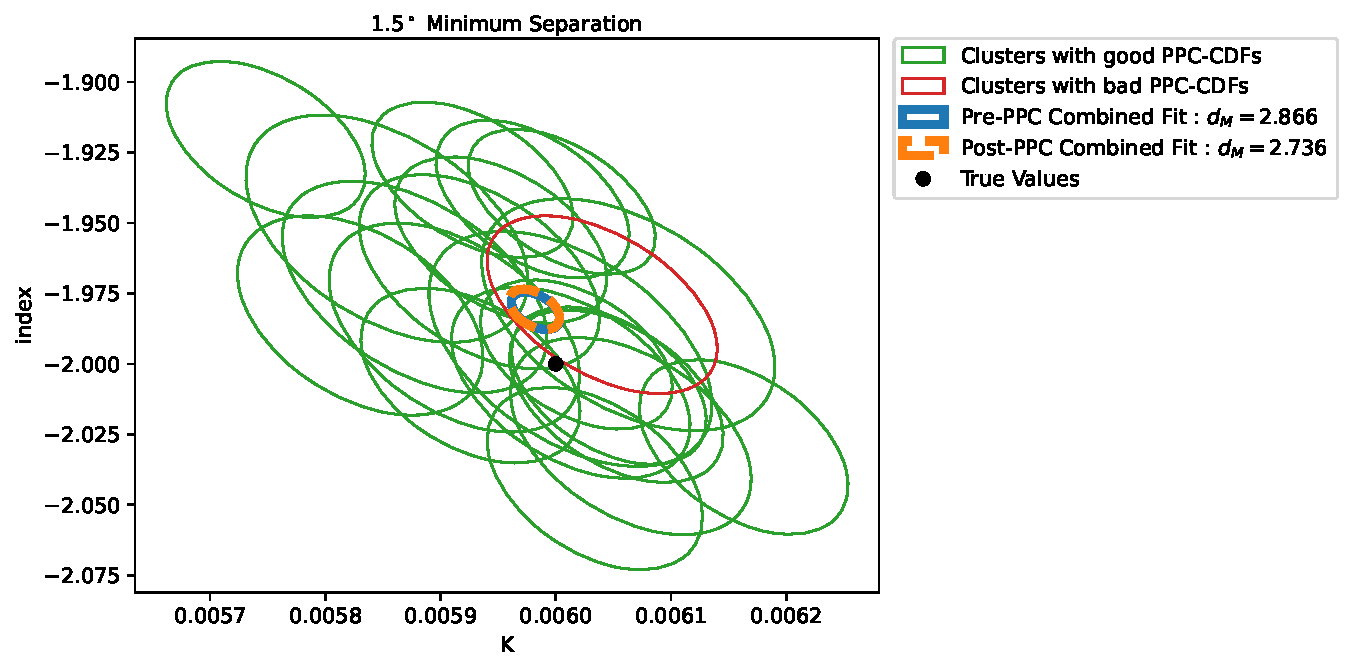
\includegraphics[width=\textwidth]{Images/PPC_and_Background_Analysis/combined_plot_0374_ppc_normal.pdf}
  \caption{Fit results of individual pointings clusters with a minimum angular distance of $1.5^\circ$. In green are those with good PPC-CDFs and in red are those with bad PPC-CDFs. Also shown are the results of fitting all clusters together in one fit (Pre-PPC), and fitting only clusters with good PPC-CDFs together in one fit (Post-PPC).}
  \label{ppc indv fits 1.5}
\end{figure}

\begin{figure}[H]
  \centering
  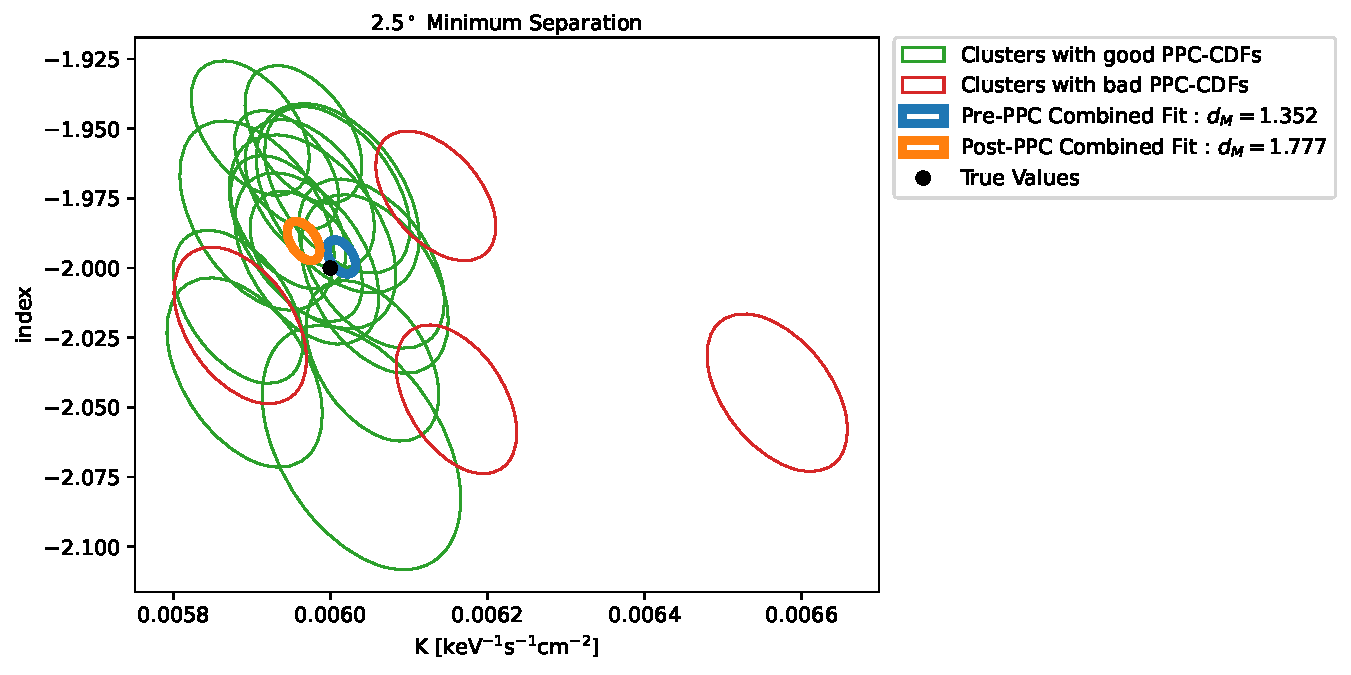
\includegraphics[width=\textwidth]{Images/PPC_and_Background_Analysis/combined_plot_0374_ppc_far.pdf}
  \caption{Analogous to figure \ref{ppc indv fits 1.5} except the minimum angular distance between pointings in a cluster is $2.5^\circ$.}
  \label{ppc indv fits 2.5}
\end{figure}


\begin{figure}[h]
  \centering
  \begin{subfigure}{0.5\textwidth}
    \centering
    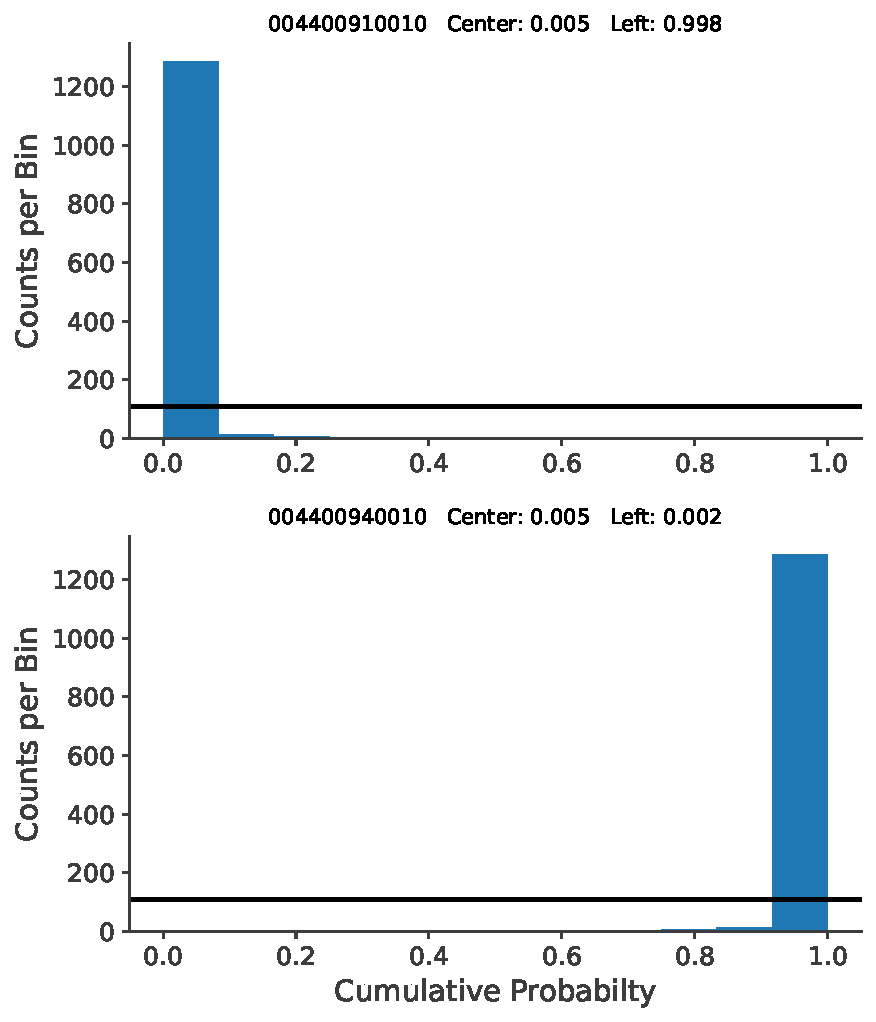
\includegraphics[width=0.9\linewidth]{Images/PPC_and_Background_Analysis/004400910010_004400940010_cdf.pdf}
    %\caption{A subfigure}
    %\label{fig:sub1}
  \end{subfigure}%
  \begin{subfigure}{.5\textwidth}
    \centering
    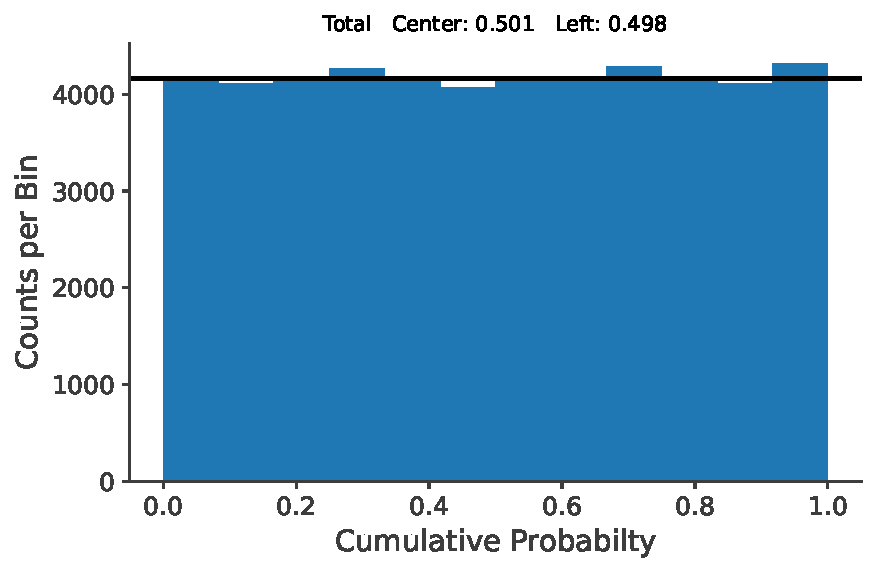
\includegraphics[width=.9\linewidth]{Images/PPC_and_Background_Analysis/Total_cdf.pdf}
    %\caption{A subfigure}
    %\label{fig:sub2}
  \end{subfigure}
  \caption{On the left a pointing cluster with an astonishingly bad CDF distribution is displayed. It is taken from a Crab Nebula fit near the end of its revolution, where it is likely caused by non-constant background rates due satellite material activation from cosmic particles as INTEGRAL nears Earth. On the right the total CDF distribution using all clusters from the mixed simulation dataset of revolution 0374 is shown.}
  \label{fig ppc really bad total}
\end{figure}

\pagebreak

\FloatBarrier

\begin{wrapfigure}{r}{0.5\textwidth}
  \vspace{-00pt}
  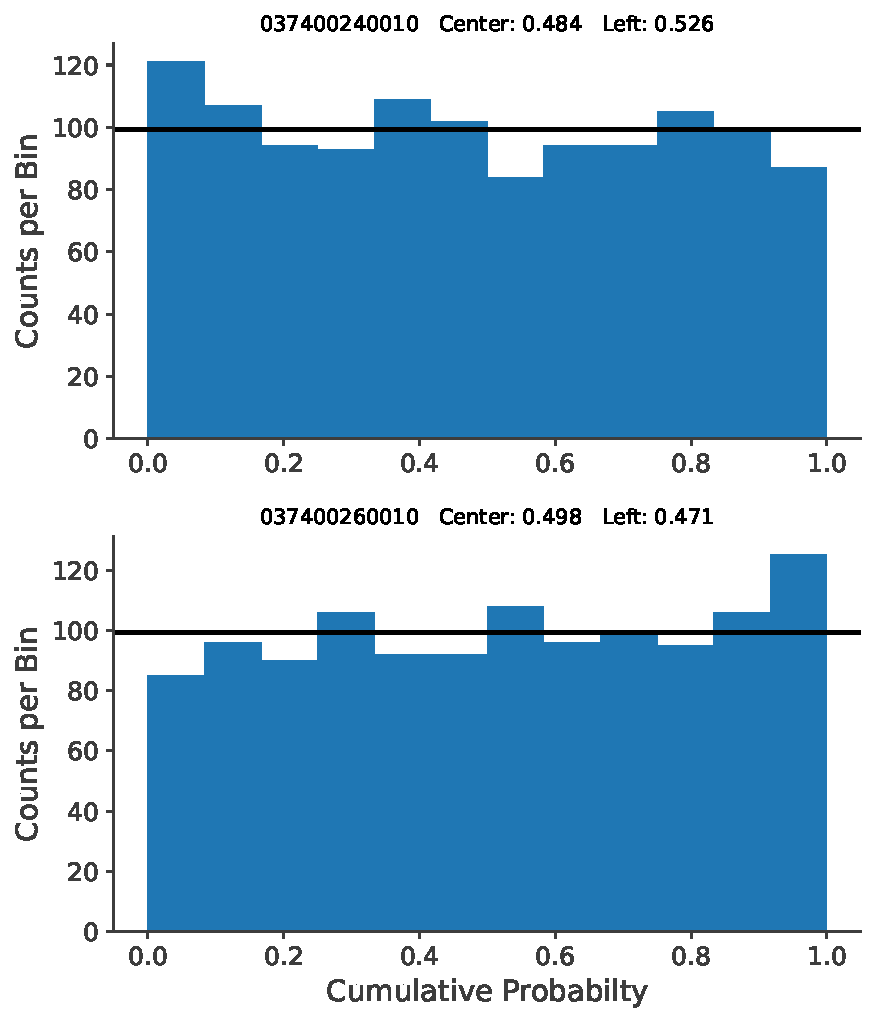
\includegraphics[width=\linewidth]{Images/PPC_and_Background_Analysis/037400240010_037400260010_cdf.pdf}
  \vspace{-00pt}
  \caption{Example CDF distribution where it is not inherently clear if the CDF distribution is acceptably good or not.}
  \vspace{-150pt}
  \label{fig ppc mediocre}
\end{wrapfigure}

Deciding which CDF distributions are acceptable or unacceptable is an inherently subjective task. For distributions as seen in figure \ref{fig ppc cdf ex good and bad} it is an easy choice, but there are many cases where it is not as simple. Figure \ref{fig ppc mediocre} shows a CDF distribution with an unmistakable asymmetry towards the left and right end of the spectrum. One could argue that this indicates (amongst other possibilities) a non-constant background rate between the two SCWs in the cluster, and the the cluster should therefore be removed from the fit. The individual fits of clusters like this show no discernable decrease in fit quality, which makes it hard to justify excluding them. The rule of thumb used in this thesis is therefore that clusters are only removed if they are very obviously identified as outliers, which the cluster from figure \ref{fig ppc mediocre} is not.




\FloatBarrier

\pagebreak

\subsection{Background Analysis} \label{sec back anal}


\begin{wrapfigure}{R}{0.45\textwidth}
  \vspace{-30pt}
  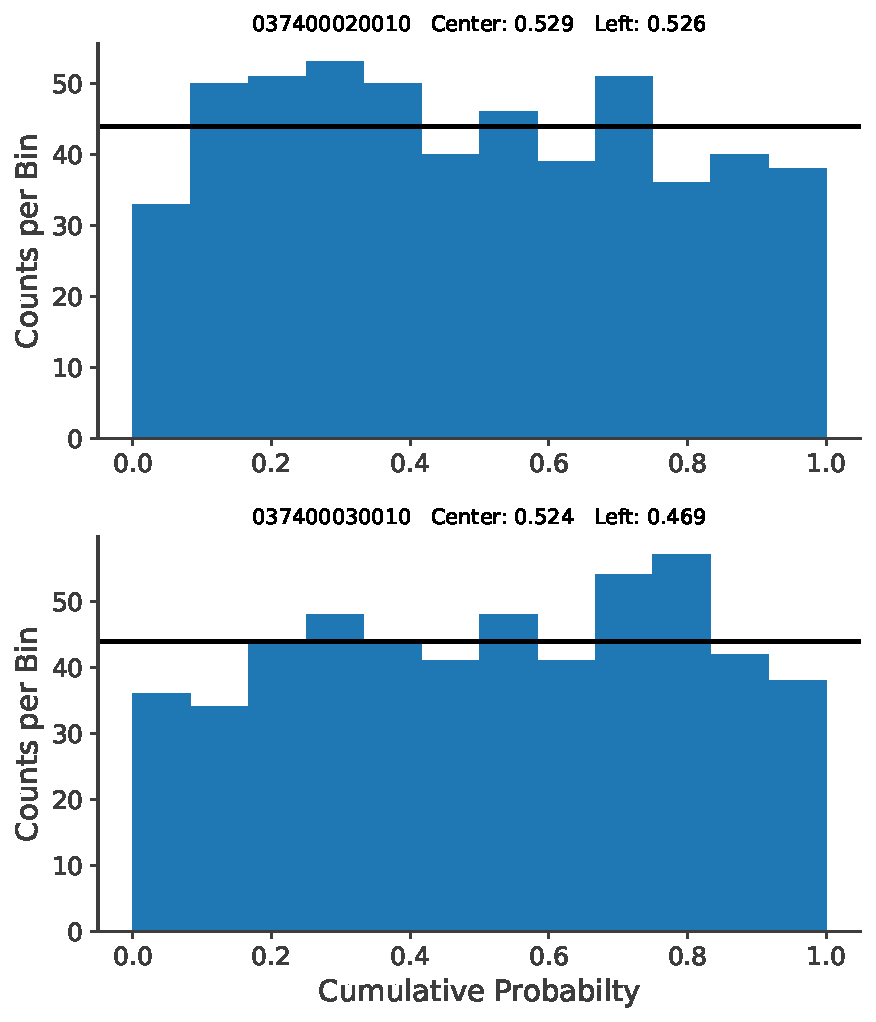
\includegraphics[width=\linewidth]{Images/PPC_and_Background_Analysis/037400020010_037400030010_cdf_smf_bkg.pdf}
  \vspace{-20pt}
  \caption{Example CDF distribution from the fit using the Spimodfit background counts along with a simulated source.}
  \vspace{+10pt}
  \label{fig smf cdf}
\end{wrapfigure}

In the previous section clusters with bad CDFs were removed from the total fits. Based on the results of fitting the clusters individually it was not always obvious what makes these clusters bad and why they should be removed, in particular for figure \ref{ppc indv fits 1.5} where the minimum pointing distance is $1.5^\circ$. To rectify this we shall now analyze the background counts in more detail.

A very useful statistical quantity is the ratio of the expected variance to the actual variance of background counts within clusters. For every energy bin per detector in every SCW cluster, we can calculate the variance of background counts between SCWs that would be expected if the counts are Poisson distributed with a constant count-rate. Since variances of independent distributions add, the calculation is simple. Based on the different lifetimes there is a natural variance in the expected counts (which needs to be Bessel corrected) that is added to the variance of two Poisson distributions:

\begin{equation}
  E(var) = (rt_1 - m)^2 + (rt_2 - m)^2 + \frac{r(t_1+t_2)}{2}
\end{equation}
where $r=\frac{C_1+C_2}{t_1+t_2}$ is the average count-rate in both energy bins, $m=\frac{C_1+C_2}{2}$ is the average number of counts, and $t_1$ and $t_2$ are the lifetimes of the respective SCWs. It is then possible to take the ratio of the actual variances of counts to the expected variances, and to plot the distribution of the ratios for all bins and all clusters in a fit. If the actual counts really are Poisson distributed from a constant background rate within clusters, then the ratio is expected to be 1. If the background rates are not equal for all SCWs in each cluster then the ratio will be larger than 1.

This is shown in figure \ref{fig back var} for the mixed simulation count spectra from the previous section using real background counts and a simulated source for both configurations of the minimum angular distance between pointings. As theorized, the mean variance ratio for clusters with a minimum distance of $1.5^\circ$ is much lower at 1.052 than the corresponding mean variance ratio for clusters with a minimum distance of $2.5^\circ$ at 1.151, indicating that the larger time windows between SCWs do lead to a substantial change in background count rates. Furthermore, when removing clusters with bad CDFs from the fit the mean variance ratio for both cluster sets drops significantly to 1.016. This tells us that only a few clusters suffer from the issue of non-constant background rates, and that these are the clusters that result in bad CDFs. For a minimum distance of $2.5^\circ$ there are more clusters with non-constant background and the change in background is larger. These clusters are easily identified and removed, resulting in a set of clusters with equally constant background rates for both configurations of the minimum distance.

Also shown in figure \ref{fig back var} is the variance ratio of the Spimodfit produced background. The variance ratio is very similar to that of the real background. Curiously, the PPC analysis did not yield very decisive results (see figure \ref{fig smf cdf}) here. This is thought to be a result of the Spimodfit background being binned into larger energy-bins than those used for PySPI fits, resulting in less data-points and hence a larger variance in the CDF distribution. In order for the CDF distributions to be useful, a sufficient number of energy bins is required.

Lastly, figure \ref{fig back var} shows the variance ratio of revolution 1662, observing the Crab Nebula, for comparison purposes. Since these are real data counts, we cannot calculate the variance ratio for just the background counts, but have to include source counts as well. As expected, the inclusion of source counts means the count rates are no longer purely Poisson distributed, resulting in larger variance ratios. 

Note that the peak around 1 is caused by SCW clusters with very different lifetimes. This increases both the expected and actual variance, thus resulting in ratios distributed much more tightly around 1.



\begin{figure}[h]
  \centering
  %\vspace{-30pt}
  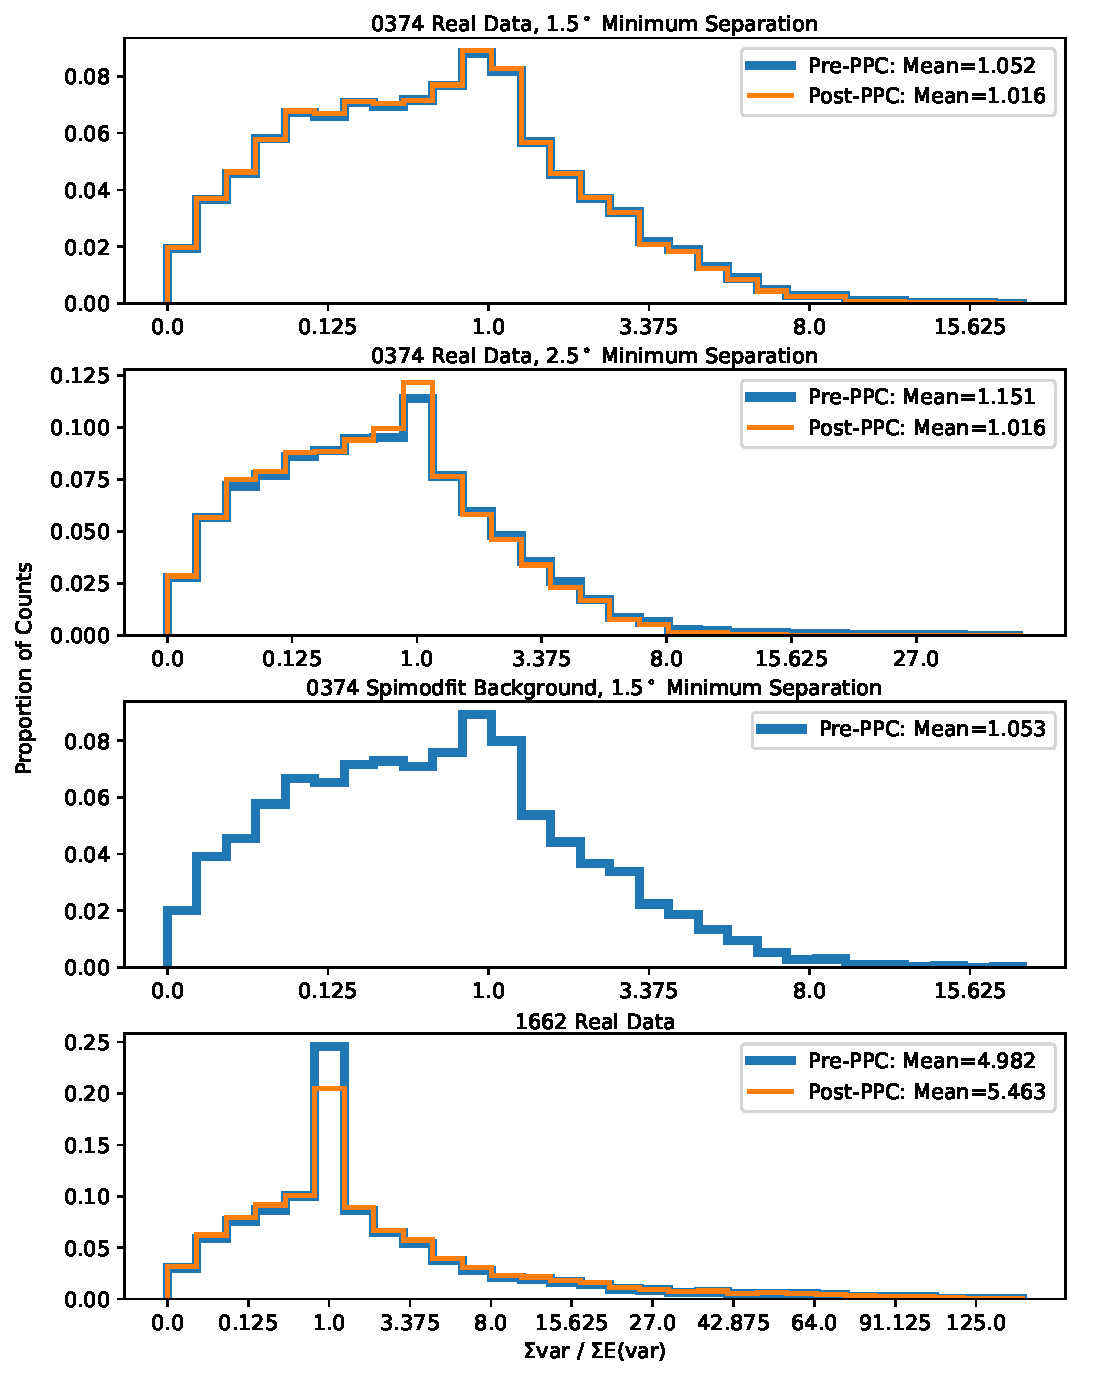
\includegraphics[width=\textwidth]{Images/PPC_and_Background_Analysis/background_variance.pdf}
  \caption{The ratio of actual to expected count variance within clusters. This is shown for the real counts from revolution 0374, used as background in mixed simulations, the Spimodfit background counts, and data from revolution 1662, which includes source counts from the Crab Nebula. Also shown is how the distributions change when clusters with bad CDF distributions are removed.}
  %\vspace{-50pt}
  \label{fig back var}
\end{figure}

\FloatBarrier

\subsubsection{Background Spectrum}

\begin{figure}[h]
  \centering
  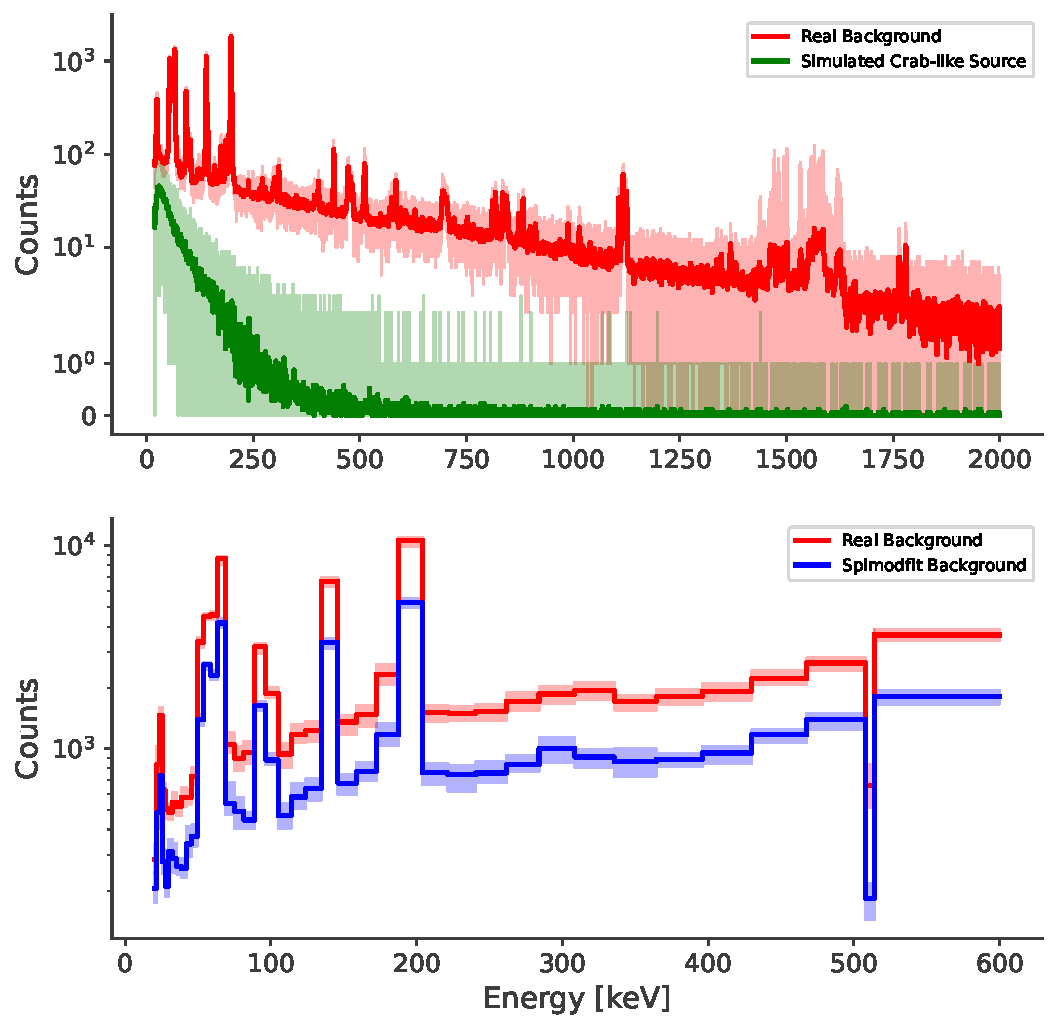
\includegraphics[width=\textwidth]{Images/PPC_and_Background_Analysis/background_spectrum.pdf}
  \caption{Background spectrum of SCW 03740002 in comparison to count rates from a simulated source with a powerlaw spectrum similar to that of the Crab nebula. In the bottom plot, the spectrum is rebinned so that it may be compared to the spimodfit background spectrum of the same SCW. The shaded areas show the range over all detectors, whereas the solid line shows the mean over all detectors.}
  \label{fig back spec}
\end{figure}

The counts from SCW 03740002 are used very often as an example background spectrum, and duplicated to other SCWs in the revolution for a constant background. Hence, it can be beneficial to visualize this spectrum, as was done in figure \ref{fig back spec}. Two things worth noting are that the counts from the simulated Crab-like source are significantly lower than those from the background, especially at higher energies, and that the Spimodfit background spectrum, although very similar in shape, is consistently smaller than the real background by a roughly constant factor. Spimodfits background model is fitted to the data based on its database of detector patters (see section \ref{about smf}). The spimodfit background model shown here and used in the mixed simulations is produced before the actual fit is conducted, which is why it is not surprising that its absolute magnitude is differs from the true background spectrum quite substantially. 


\chapter{Results}

Having tested the quality and limitations the PySPI fitting procedure for purely simulated spectra and mixed simulations, in addition to having developed a methodology for removing bad SCW clusters using PPC analysis, it is now time to apply the acquired knowledge while fitting real astronomical sources.

Refer to appendix \ref{chp source models} regarding the functions and their parameters of the different source models that will be used in the following sections.

\section{Crab Nebula}
Located in the constellation of Taurus, the Crab Nebula is a supernova remnant and pulsar wind nebula. It us well known for being one of the very few bright sources in the Hard X-ray domain with a persistent spectrum. For this reason its measurements are often used as benchmarks by instruments active in this energy range. Some instruments even used it for calibration purposes, although more recent measurements of its spectral parameters do show small variations in its emission flux on the timescales of a few years \cite{2020ApJ...899..131J}. This makes it an excellent candidate to test PySPIs fitting capabilities with over INTEGRALS long mission duration. 

It is well known that the Crab spectrum matches the approximate shape of a powerlaw with $index\approx-2$. At higher energies the index is known to decrease slightly to a steeper spectrum. Many different functions and models have been fitted to better match the Crab's spectral shape with varying success, some of which will be recreated below. The Crab Nebula is also small enough to be approximated as a point-source for SPI.

The Be puslsar 1A0535+262 is just $4.3^\circ$ away from the Crab Nebula. Usually it is orders of magnitudes dimmer than the Crab Nebula, but during flaring periods it can reach very high emission fluxes \cite{2020ApJ...899..131J}. It will have to be included in the source model of every Crab fit, and revolutions with high flux should be excluded from the Crab analysis since approximating its spectrum as a powerlaw is surely insufficient at high luminosities. 



The general procedure for fitting the Crab Nebula is the following:
\begin{enumerate}
  \item Identify groups of neighboring revolutions including as many SCWs with the Crab in SPIs field of view as possible.
  \item Fit every single revolution individually. As a source model use a powerlaw for both the Crab Nebula and the pulsar 1A0535+262.
  \item Exclude every revolution where the flux of the pulsar 1A0535+262 exceeds 1\% of the Crab's ($>$10mCrab). Since the posterior distribution for the puslars spectral parameters can look very messy, a little bit of guesswork may be required. In unclear cases the revolution is removed to stay on the side of safety.
  \item Go through the CDF distribution of every single cluster of every revolution and remove clusters with bad CDFs from further analysis. This only applies to PySPI, not Spimodfit.
  \item Group the remaining clusters from neighboring revolutions together to be fitted again with a Crab source model of choice (including the Be pulsar).
\end{enumerate}
Table \ref{tab excl revs} gives an overview of which revolutions were excluded and which revolutions are grouped together in the following sections. 

\begin{table}[h] 
  \begin{center}
  \begin{tabular}{|c|c|c|}
  \hline
  \textbf{Date}  & \textbf{Used Revolutions}    & \textbf{Excluded Revolutions} \\ \hline
  February 2003   & 43, 44, 45                   &                               \\ \hline
  March 2006     & 422                          &                               \\ \hline
  March 2008     & 665, 666                     &                               \\ \hline
  September 2010 &                              & 966, 967, 970                 \\ \hline
  March 2013     & 1268, 1278                   & 1269                          \\ \hline
  August 2013    & 1327                         & 1328                          \\ \hline
  October 2014   &                              & 1461, 1462, 1466, 1468        \\ \hline
  March 2015     & 1516, 1520, 1528             & 1515                          \\ \hline
  October 2015   &                              & 1593, 1597, 1598, 1599        \\ \hline
  March 2016     & 1657, 1658, 1661, 1662, 1664 & 1667                          \\ \hline
  February 2017  & 1781, 1784, 1785, 1789       &                               \\ \hline
  August 2017    &                              & 1850, 1856, 1857              \\ \hline
  February 2018  & 1921, 1925, 1927, 1930       &                               \\ \hline
  September 2018 & 1996, 1999, 2000             &                               \\ \hline
  February 2019  & 2058, 2062, 2063, 2066       &                               \\ \hline
  \end{tabular}
  \end{center}
  \caption{}
  \label{tab excl revs}
\end{table}

\FloatBarrier



\subsection{Powerlaw}
\begin{figure}[h]
  \centering
  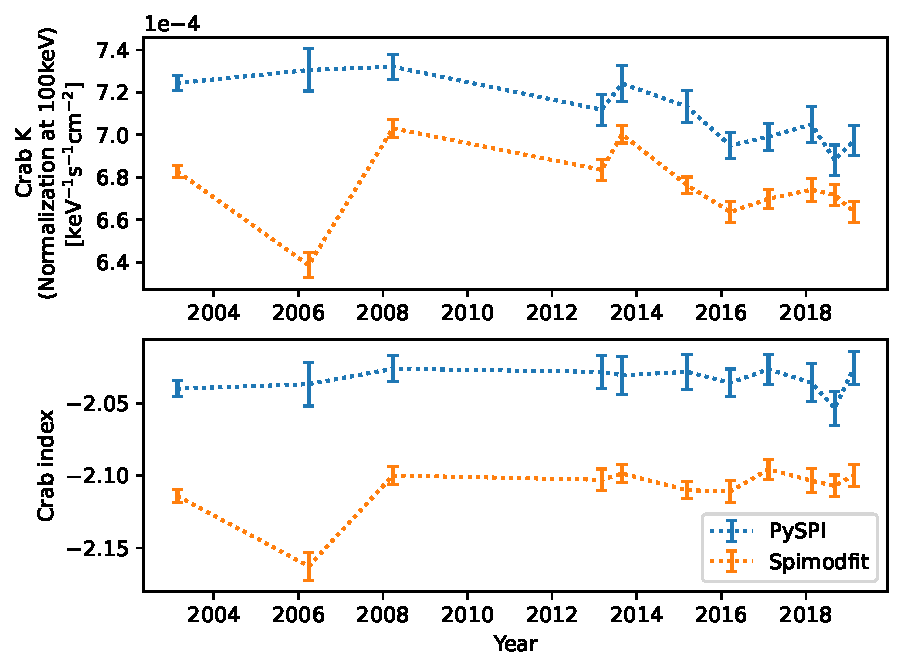
\includegraphics[width=0.75\textwidth]{Images/Crab_Fits/crab_low_energy_pl.pdf}
  \caption{The Crab Nebula fitted as a powerlaw in the energy range 30-81-5keV using PySPI and Spimodfit. Despite being listed as excluded in table \ref{tab excl revs} due to a large flux of the pulsar 1A0535+262, fits from September 2010 are included in this figure since they provide crucial insight into the Crab "fading" in this time period. The effect of the pulsar is probably insignificant on the fit, but the data-point should be viewed with extra caution regardless.}
  \label{fig crab pl}
\end{figure}

\begin{figure}[h]
  \centering
  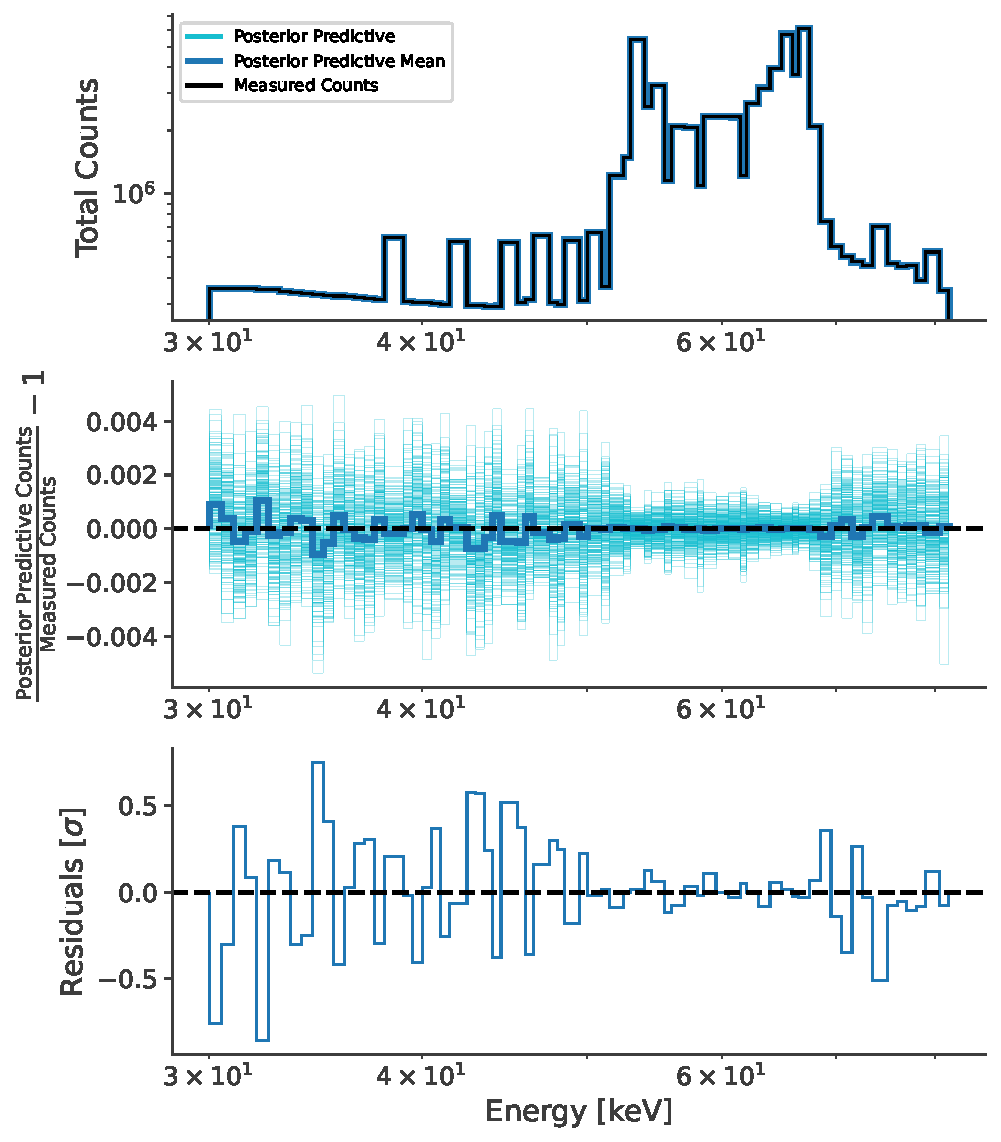
\includegraphics[width=0.8\textwidth]{Images/Crab_Fits/energy_residual_plot_pl.pdf}
  \caption{PySPI energy dependant count spectrum and residuals using a powerlaw source model and revolutions from February 2003.}
  \label{fig res pl}
\end{figure}

To begin with, the Crab Nebula is fitted as a simple powerlaw (equation \ref{powerlaw}) using both PySPI and Spimodfit (figure \ref{fig crab pl}). Since the powerlaw index is know to change at high energies the fits are limited to an energy range of 30-81.5keV. PySPI sees the Crab with higher flux (at 100keV) and with smaller index across the entire duration. The temporal evolution is very similar for both fitting methods, with the normalization decreasing slightly and the indices staying constant. Spimodfit records a curious dip in luminosity and index in early 2006 where PySPIs parameters remain constant.

The energy dependant count spectrum and residuals for the PySPI fit from February 2003 is shown in figure \ref{fig res pl}. The fit matches the measured count spectrum well for all energies, although a very slight tendency towards negative residuals at both ends of the spectrum is observable. This is expected due to the known behavior that the index decreases at high energies.





\begin{table}[]
  \centering
  \begin{tabular}{|c|c|c|}
  \hline
  \textbf{Instrument}         & \textbf{Index} & \textbf{50-100keV flux {[}s$^{-1}$cm$^{-2}${]}} \\ \hline
  OSO-8                       & $-2.00\pm0.06$ & $6.41\cdot 10^{-2}$                             \\ \hline
  GRIS                        & $-2.15\pm0.03$ & $4.52\cdot 10^{-2}$                             \\ \hline
  CGRO/OSSE                   & $-2.19\pm0.03$ & $5.68\cdot 10^{-2}$                             \\ \hline
  CGRO/BATSE                  & $-2.20\pm0.01$ & $6.83\cdot 10^{-2}$                             \\ \hline
  SAX/PDS                     & $-2.13\pm0.01$ & $4.92\cdot 10^{-2}$                             \\ \hline
  INTEGRAL/SPI - Sizun (2004) & $-2.17\pm0.01$ & $7.08\cdot 10^{-2}$                             \\ \hline
  INTEGRAL/SPI - PySPI        & $-2.08\pm0.03$ & $7.26\cdot 10^{-2}$                             \\ \hline
  INTEGRAL/SPI - Spimodfit    & $-2.12\pm0.03$ & $7.05\cdot 10^{-2}$                             \\ \hline
  \end{tabular}
  \caption{Crab Nebula Powerlaw parameters from various instruments and different SPI methods \cite{sizun2004integralspi}. The revolutions used for the SPI analysis are from February 2003.}
  \label{tab crab comparison}
\end{table}

Table \ref{tab crab comparison} shows the powerlaw indices and integrated fluxes from 50 to 100keV as measured by several different instruments \cite{sizun2004integralspi}. It is worth noting that the indices between from PySPI and Spimodfit are not directly comparable to others listed, since the PySPI and Spimodfit fits only used the energy range of 50-100keV, whereas other methods listed in the table used the entire available gamma energy range. This explains the notably lower indices for PySPI and Spimodfit. The measured fluxes should be relatively unaffected by this. Once again, PySPI measures a significantly brighter Crab than other methods. Spimodfit agrees well with other the SPI method \cite{sizun2004integralspi}. Other instruments measure varying, yet consistently dimmer fluxes.

\subsubsection*{Crab "Fading"}

\begin{figure}[h]
  \centering
  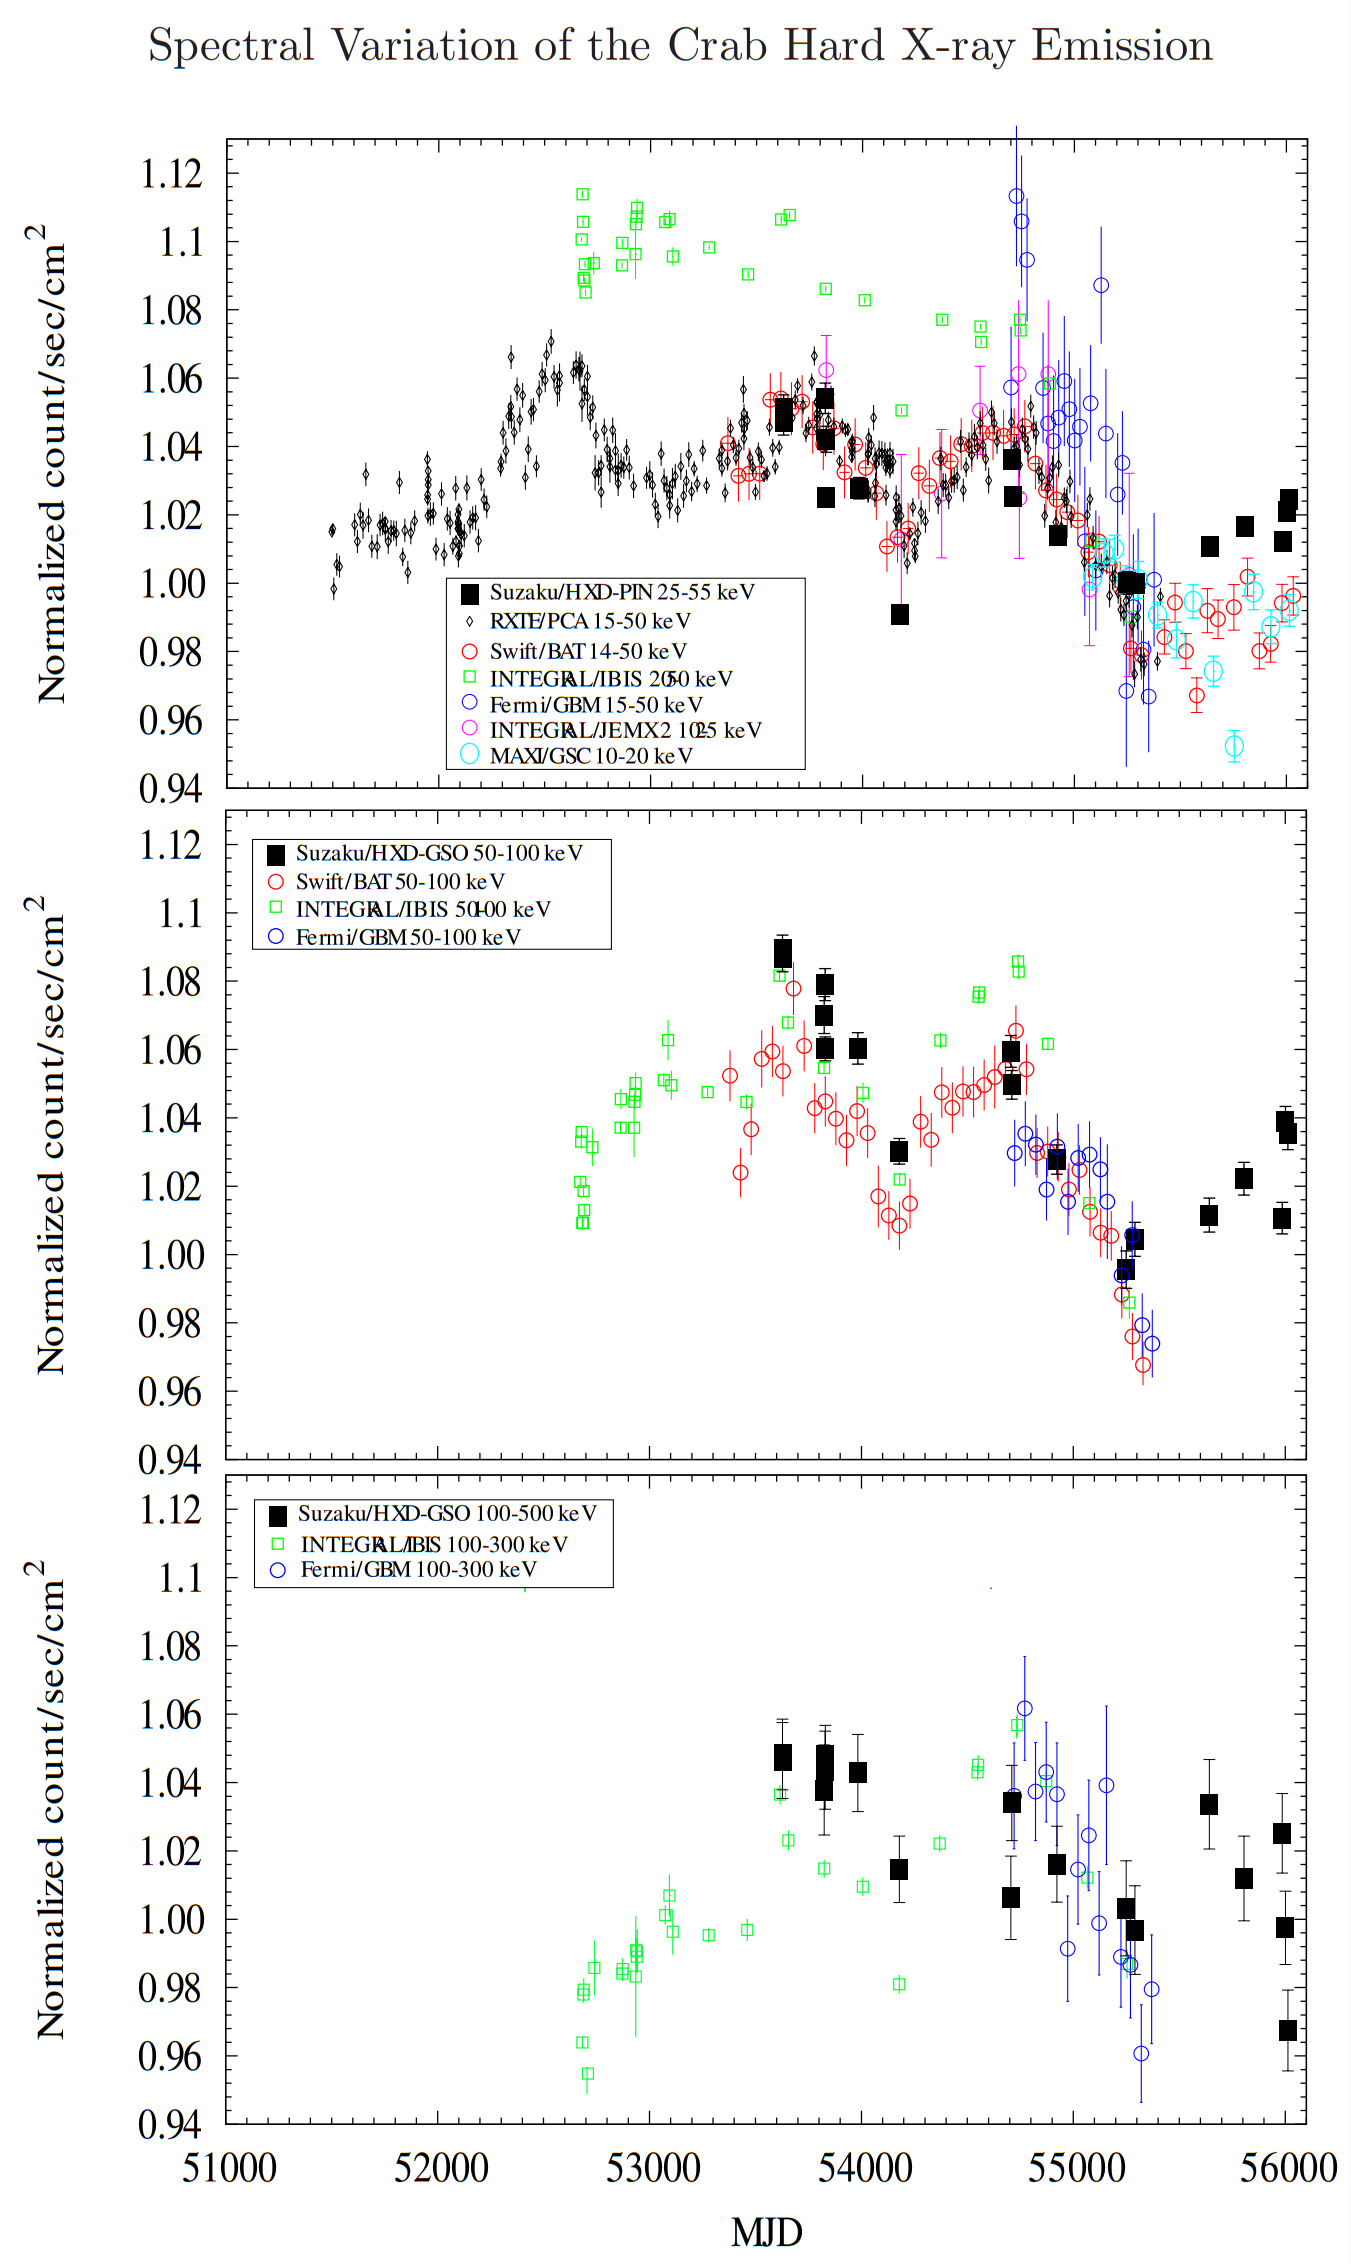
\includegraphics[width=0.75\textwidth]{Images/Crab_Fits/Crab_light_curve.PNG}
  \caption{Crab Nebula light-curves using data from several different instruments overlapped and in three different energy ranges \cite{sizun2004integralspi}. The data covers a time range from July 1998 (MJD 51000) to March 2012 (MJD 56000).}
  \label{fig crab light curve}
\end{figure}

Figure \ref{fig crab light curve} shows light curves of several instruments for the Crab Nebula. The Crab "fading", resulting in a significant reduction of its flux around 2010 is clearly visible. We may compare the flux reduction from March 2008 to September 2010 of the instruments shown in this figure to those measured in the PySPI and Spimodfit fits. According to figure \ref{fig crab light curve} the flux reduces by 5 to 7.5\%, depending on which instruments are used. The corresponding PySPI fits show a flux decrease of 6\%, and for Spimodfit we find a decrease of 5\%. The extend of the decreases in Crab flux measured using the different methods are therefore cohesive.

Initial theories considered the Crab flux variability as a result of instrumental effects. However, since the measured flux decrease is so consistent amongst different instruments this can be ruled at, and the flux variability is determined to be inherent to the Crab Nebula \cite{Wilson_Hodge_2011}. INTEGRAL proved to be particularly important in this observation as its highly elliptical orbit places it well above Earth's atmosphere and any effects related to it.

One model capable of explaining the observed time variability relates to the Crab pulsar wind flow based on magnetohydrodynamic simulations \cite{10.1111/j.1365-2966.2009.15550.x}. It models the Crab Nebula as an archetypal compact synchrotron nebula, caused by a rapidly rotating neutron star creating magnetized, ultrarelativitic wind. The wind is decelerated at a termination shock with a radius such that the pressure of the pulsar wind equals the surrounding pressure. The wind plasma is heated by the termination shock, resulting in bubbles of relativistic particles known as a pulsar wind nebula. Adiabatic and synchrotron losses, detectable as non-thermal radiation, produce inhomogeneous variations in the  magnetic field that ultimately travel through the shock diameter at relativistic speeds for 1-2 years, matching up with observed Crab Nebula behavior \cite{Wilson_Hodge_2011}.

Another, similar, model also based on magnetohydrodynamic simulations \cite{Spitkovsky_2004}, states that the inhomogeneity in the wind plasma on scales of the ion Larmor radius is caused by the relativistic cyclotron instability of the ion gyrational orbit. This results in cyclical compressions of the electron-positron plasma. The simulations predict flux variations on similar timescales to those observed in the Crab Nebula \cite{Wilson_Hodge_2011}.

Since the relative flux variability measured using PySPI agrees well with previous measurements, these models cannot be disputed with the new fits.



\FloatBarrier

\subsection{Broken Powerlaw}

\begin{figure}[H]
  \centering
  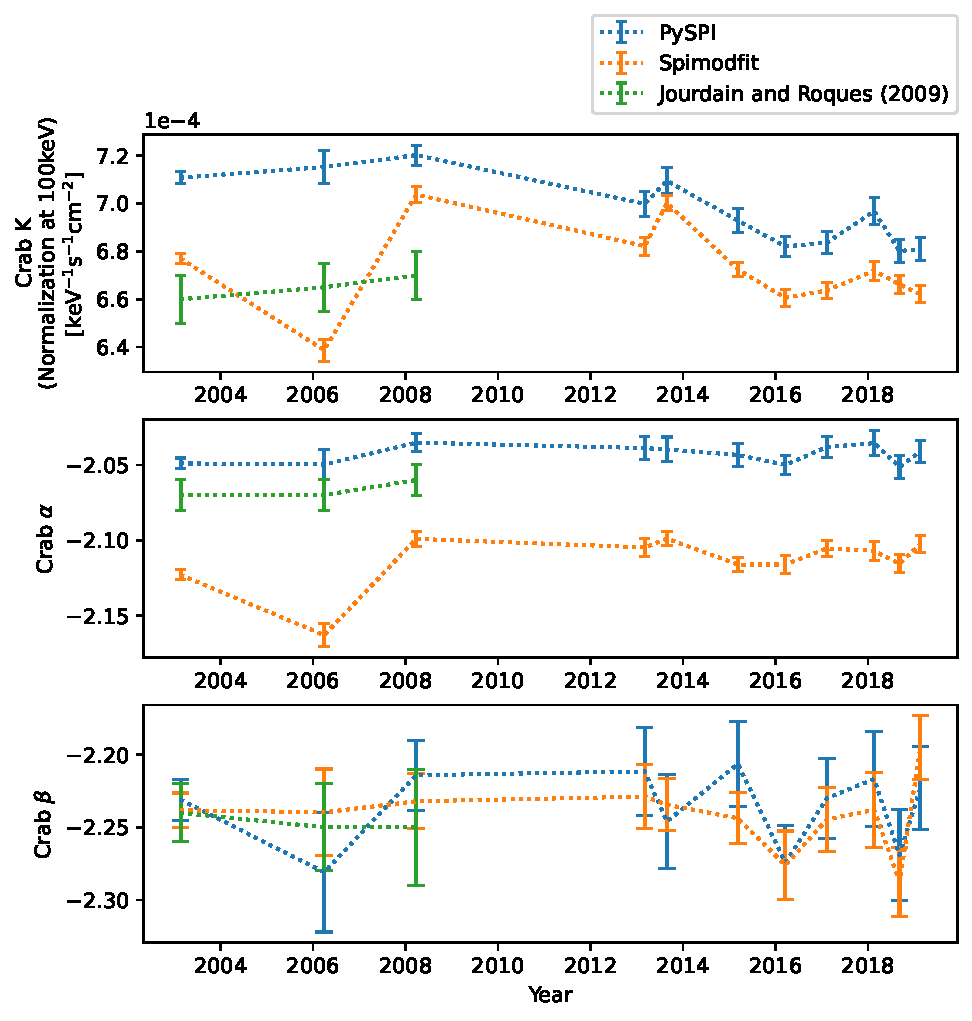
\includegraphics[width=.65\textwidth]{Images/Crab_Fits/crab_brk_pl_100.pdf}
  \caption{The Crab Nebula fitted as a broken powerlaw with the break energy $x_b$ fixed at 100keV. Shown are fit results for PySPI, Spimodfit, and published results by Jourdain and Roques (2009) \cite{2009ApJ...704...17J}.}
  \label{fig crab br pl}
\end{figure}

\begin{figure}[h]
  \centering
  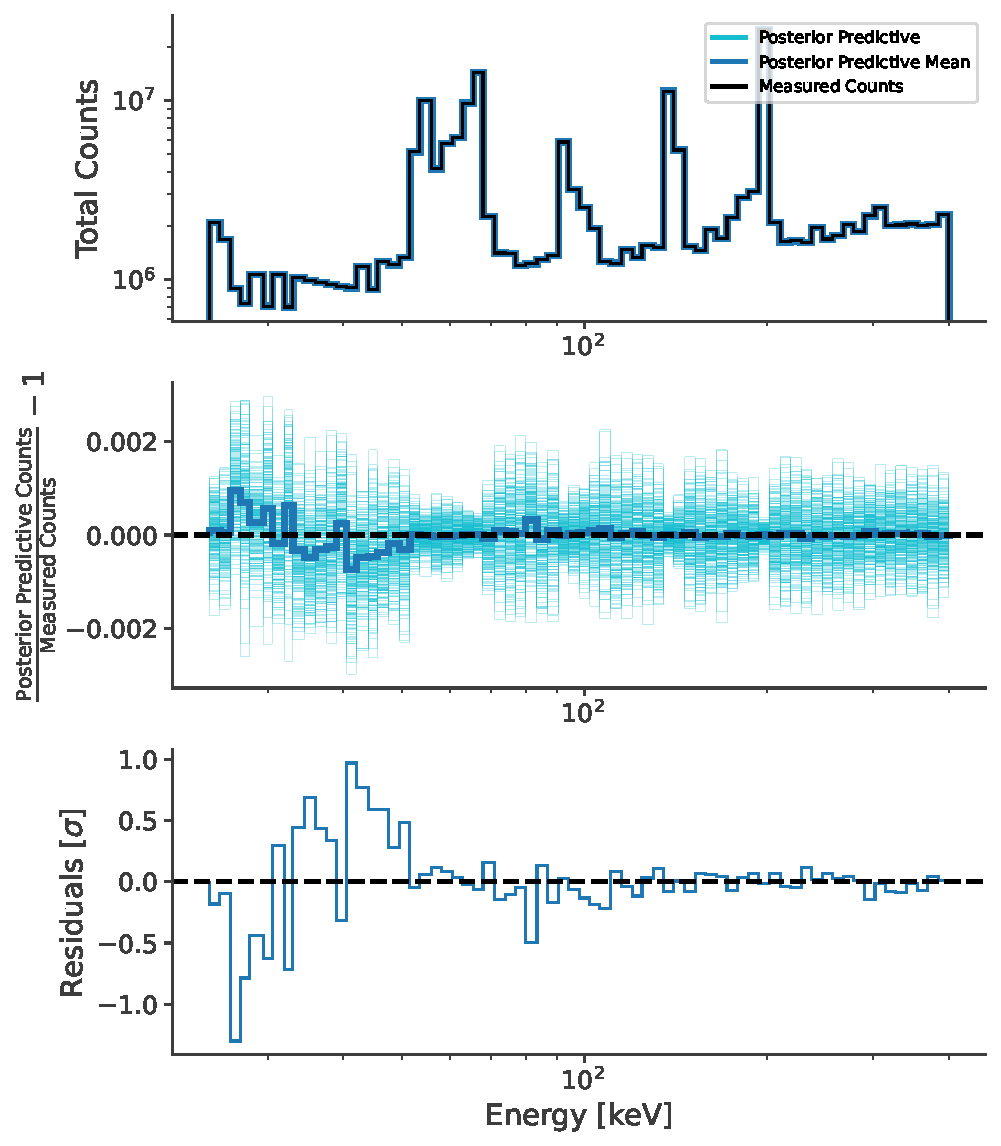
\includegraphics[width=0.5\textwidth]{Images/Crab_Fits/energy_residual_plot_br_pl_100.pdf}
  \caption{PySPI energy dependant count spectrum and residuals using a broken powerlaw source model (with the break energy fixed at 100keV) and revolutions from February 2003.}
  \label{fig res br pl}
\end{figure}

Next up a broken powerlaw (equation \ref{eq br pl}) is used in the source model for the Crab Nebula, which allows us to use higher energies: up to 400keV are included in the fits. The break energy $x_b$ is fixed at 100keV. This specific source model was chosen intentionally as it allows a direct comparison with Jourdain and Roques (2009) \cite{2009ApJ...704...17J}, who used the same model in corresponding fits (see figure \ref{fig crab br pl}). It is worth noting that the fits aren't exactly comparable, since  Jourdain and Roques (2009) \cite{2009ApJ...704...17J} used an energy range up to 6MeV and also included more INTEGRAL revolutions (depending on the fit).

Once again PySPI determines the Crab to have higher flux and a smaller low-energy powerlaw index, and the trend constant indices but slightly decreasing flux is observed again as well. Fits by Jourdain and Roques (2009) \cite{2009ApJ...704...17J} are closer to Spimodfit as far as normalization is concerned, but show a low-energy index closer to PySPIs. The high-energy index is similar for all three methods.

The energy dependant count spectrum and residuals for the PySPI fit from February 2003 is shown in figure \ref{fig res br pl}. The fit matches the measured count spectrum well for high energies. At very low energies the residuals are notably negative, and at energies slightly above the residuals are notably positive. This indicates the the fixed break energy of 100keV used in the fit could be placed at a larger than optimal energy.



\FloatBarrier

\subsection{Band Function}

\begin{figure}[h]
  \centering
  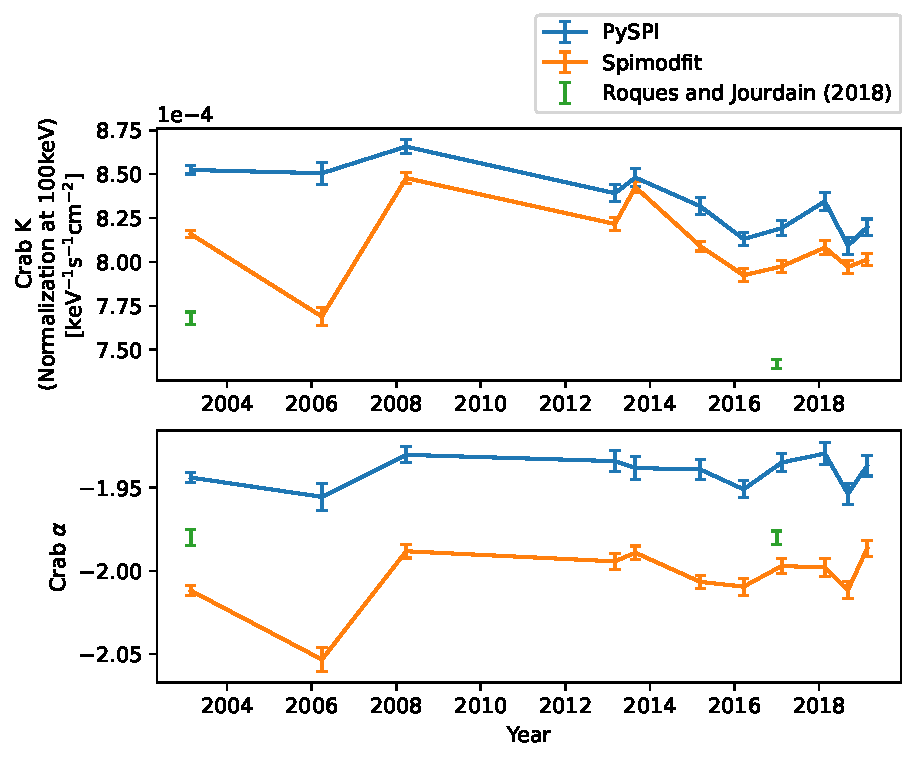
\includegraphics[width=.65\textwidth]{Images/Crab_Fits/crab_c_band.pdf}
  \caption{The Crab Nebula fitted using the Band function with fixed characteristic $x_p$ at 500keV. Since PySPI and Spimodfit are only fitted using data up to 400keV, only the low-energy index $\alpha$ and normalization $K$ are included as fit parameters. Also shown are the results by Roques and Jourdain (2018) \cite{Roques}.}
  \label{fit crab c band}
\end{figure}

\begin{figure}[h]
  \centering
  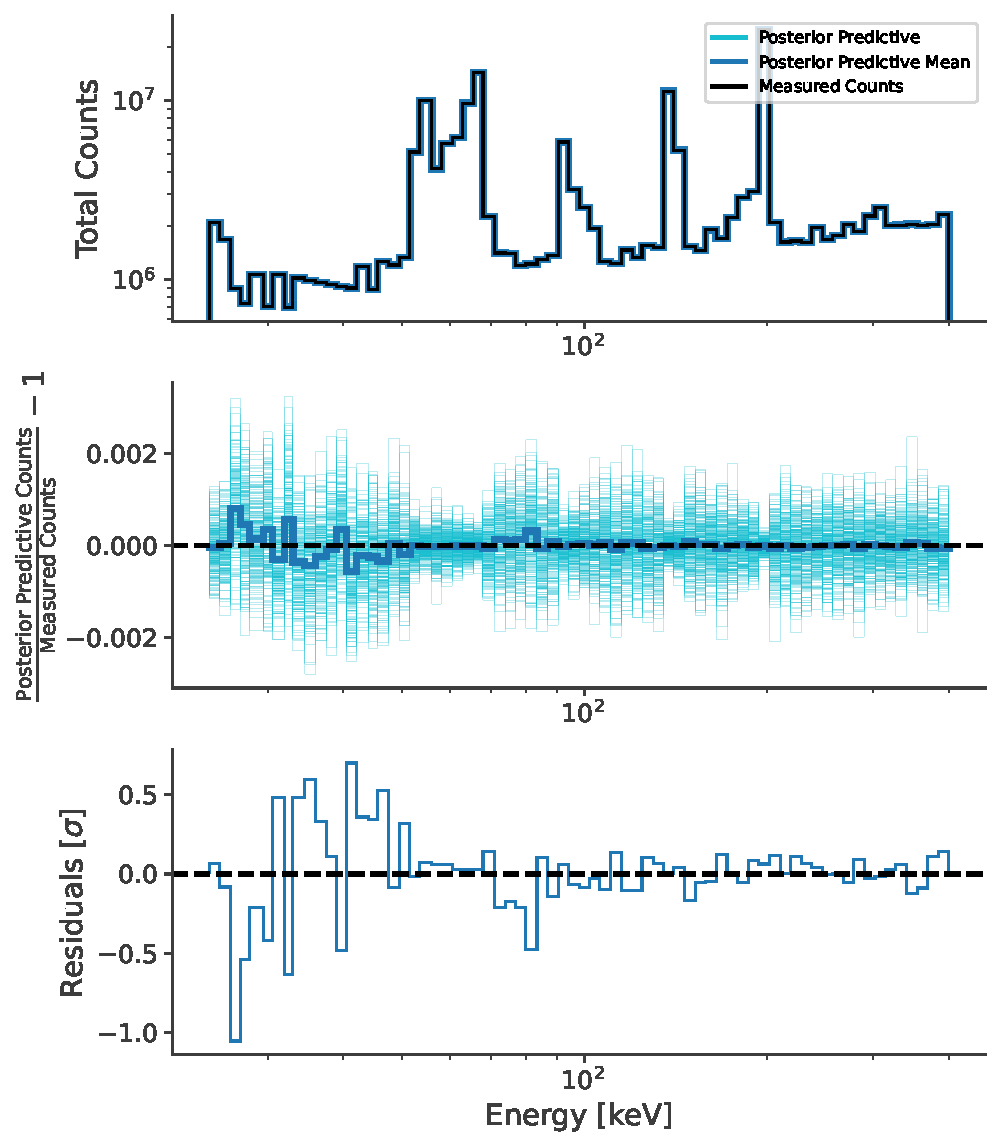
\includegraphics[width=0.55\textwidth]{Images/Crab_Fits/energy_residual_plot_lower_band.pdf}
  \caption{PySPI energy dependant count spectrum and residuals using a band function source model (with the critical energy fixed at 500keV) and revolutions from February 2003.}
  \label{fig res band}
\end{figure}

Another function that has been used to describe the Crab Nebula is the Band function (equation \ref{eq band func}). Here the Crab is fitted using a fixed characteristic energy $x_p$ at 500keV. Since data is only used up to 400keV, only the low-energy index $\alpha$ and normalization $K$ are fitted. This source model was chosen to allow comparison with Roques and Jourdain (2018) \cite{Roques}, whose results are shown alongside PySPI and Spimodfit in figure \ref{fit crab c band}. As with the broken powerlaw, the results are not exactly comparable due to Roques and Jourdain (2018) \cite{Roques} using a larger energy range and different INTEGRAL revolutions. For the selected model parameters these differences should only have a small impact, but this cannot be confirmed.

We observe similar trends to previous source models: PySPI fits result in larger flux and smaller indices compared to Spimodfit, the indices stay roughly constant over time and the flux decreases slightly. Interestingly, the flux measured by Roques and Jourdain (2018) \cite{Roques} is significantly lower than that measured by both PySPI and Spimodfit, and the low-energy index lies between the two.

The energy dependant count spectrum and residuals for the PySPI fit from February 2003 is shown in figure \ref{fig res band}. Similarly to the broken powerlaw, the source model matches the data well at high energies but predicts too many counts at very low energies and too few at energies just above that. 

\FloatBarrier

\subsection{Smoothly Broken Powerlaw}
\begin{figure}[H]
  \centering
  \makebox[\textwidth][c]{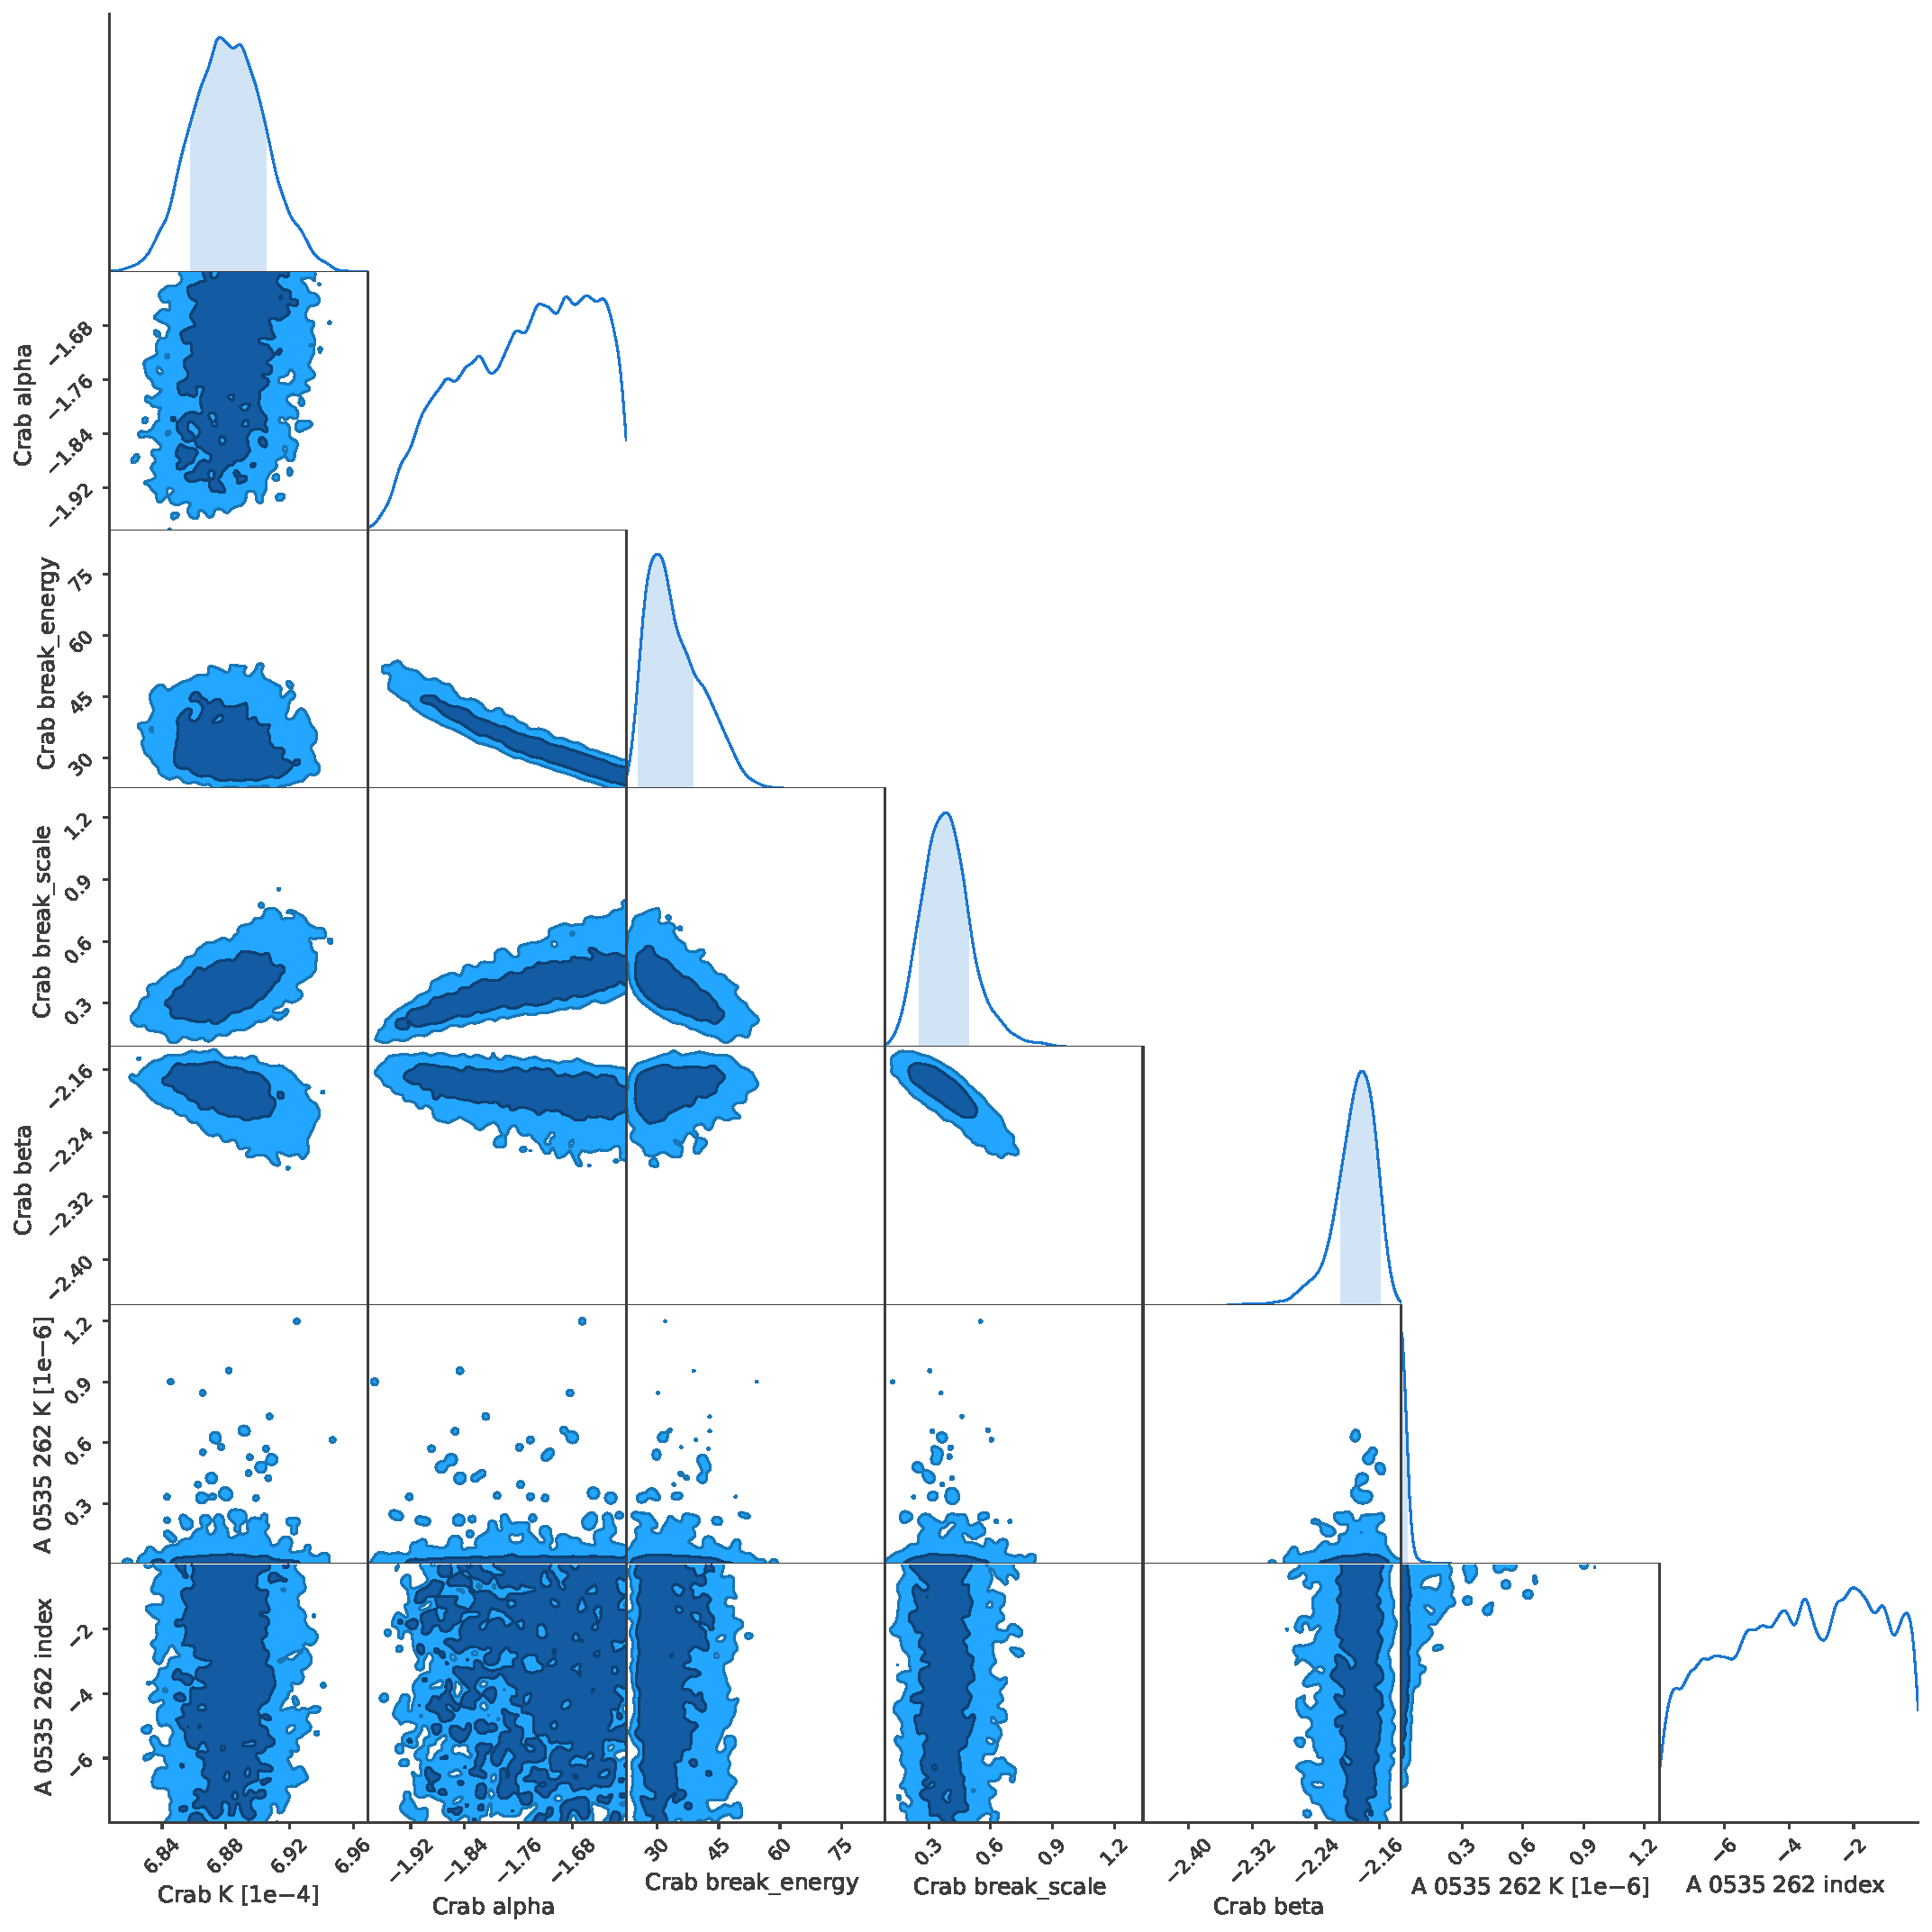
\includegraphics[width=1.1\textwidth]{Images/Crab_Fits/0043__sm_br_pl_parameters.pdf}}%
  \caption{PySPI posterior parameter distribution when fitting the Crab Nebula using a smoothly broken powerlaw. Revolutions from February 2003 are used.}
  \label{fig sm br pl fit param}
\end{figure}

\begin{figure}[h]
  \centering
  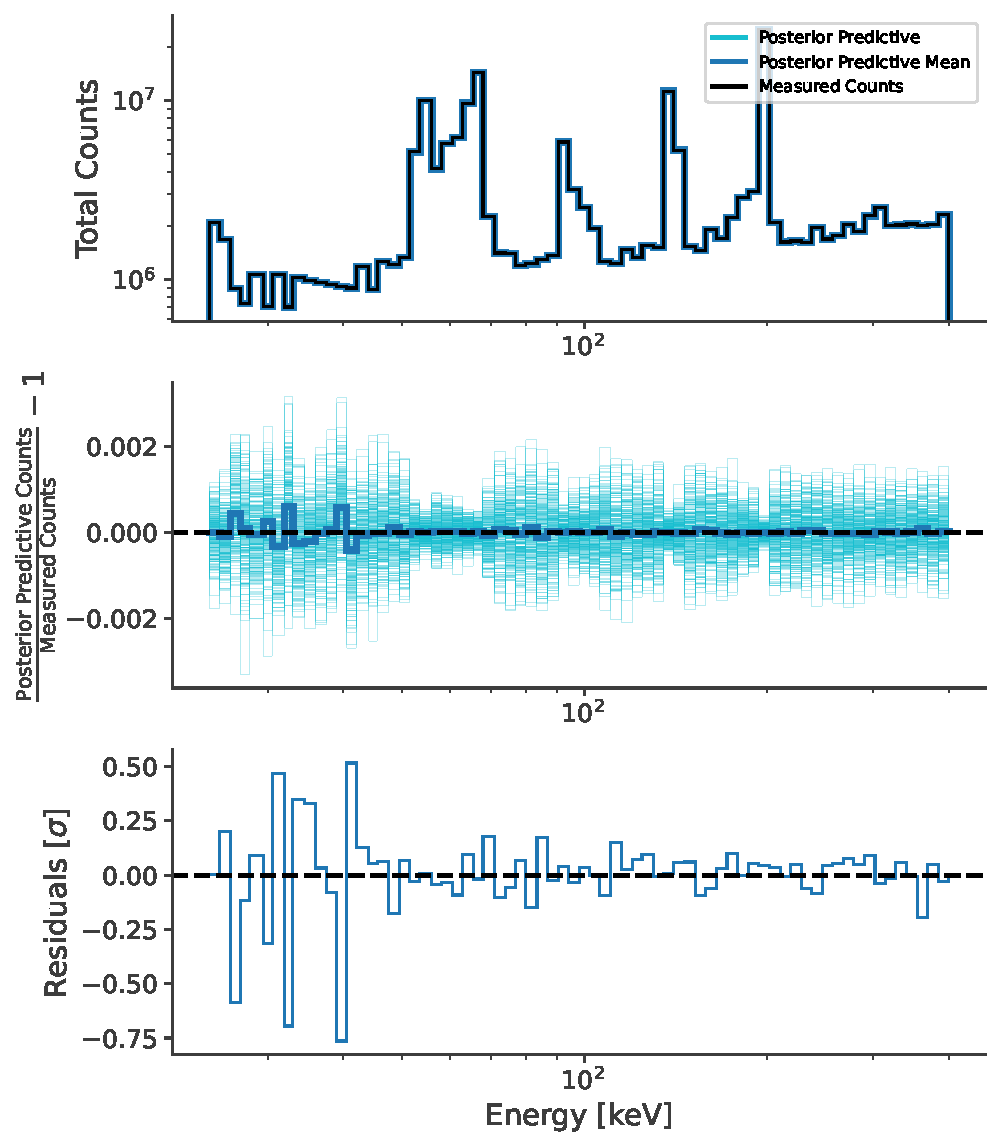
\includegraphics[width=0.6\textwidth]{Images/Crab_Fits/energy_residual_plot_sm_br_pl.pdf}
  \caption{PySPI energy dependant count spectrum and residuals using a smoothly broken powerlaw source model and revolutions from February 2003.}
  \label{fig res sm br pl}
\end{figure}

Lastly the Crab was fitted using a smoothly broken powerlaw (equation \ref{eq sm br pl}), with the break energy $x_b$ and break scale $\Delta$ as free parameters in the fit. The posterior parameter distribution for an example PySPI fit is shown in figure \ref{fig sm br pl fit param}. The parameter degeneracy for this source model is too large to offer decisive results. Particularly troublesome is the correlation between the low-energy index $\alpha$, the break energy $x_b$, and the break scale $\Delta$, where the fit has no trouble pushing the break energy outside of the used energy range and altering $\alpha$ and $x_b$ to compensate. Perhaps the fit would work better using even more revolutions in a combined fit or a larger energy range. Otherwise some of the free parameters will likely have to be fixed to predetermined values, as has been done for other some of the other models and is common practice for Crab fits. 

The energy dependant count spectrum and residuals for the PySPI fit from February 2003 is shown in figure \ref{fig res sm br pl}. The source model matches the data well across all energies. Comparatively large residuals occur at low energies, where energy bins contain fewer counts. Despite this, there is no clear tendency for positive or negative residuals. Since the parameter degeneracy of this source model is too large to result in decisive results we expect the model to match the data well. 

\chapter{Conclusion and Outlook}
The newly developed PySPI method for fitting persistent sources in SPI data was tested for under a variety of circumstances. For simulated data the fit results do not show a statistically significant systematic error, although a slight random error was observed. For mixed simulations with real background counts the fits perform well and consistently better than Spimodfit. A procedure of using PPC analysis was developed to identify and remove "bad" SCW clusters with non-constant background rates. 

If the apparent improvement, shown in section \ref{sec: smf comparison} for mixed simulations, when fitting SPI data using PySPI instead of Spimodfit are consistent across real sources, this new procedure of analyzing persistent sources would have groundbreaking implications in the astrophysical community. Not only because it would allow more accurate measurements of countless astronomical sources of interest, like providing insight into nucleosynthesis occurring in stars and novae, the distribution of important energy lines such as the 511keV line, or the processes taking place in high-energy compact objects (see section \ref{sec astrophysics with SPI}), but also because it does so at relatively low complexity. No prior knowledge of the background spectrum is required. 

The method was applied to fit the Crab Nebula using various models, obtaining slightly different parameter values compared to Spimodfit and SPI fitting methods from published papers by Jourdain and Roques \cite{2009ApJ...704...17J}\cite{Roques}. The flux variability of the Crab Nebula during its fading around 2010 was found to be similar to those of previous measurements, thus illustrating no disagreement to previous models dedicated to explaining said variability as described in Wilson Hodge (2011) \cite{Wilson_Hodge_2011}. 

There are still some issues to be solved, such as the previously mentioned random error as well as the large systematic error that appears when fitting very steep powerlaw models with insufficiently small instrument response matrices. The method may be further developed by implementing fits with larger cluster sizes (currently only clusters of size two and three can be fitted), which also requires implementing the corresponding PPC interpolation framework (currently only implemented on clusters of size two). Extending the functionality to being able to use pulse shape discriminated events is also very important, as opposed to only using single events that effectively limit the available energy range to below 400keV due to SPIs spurious events. Furthermore the procedure may be generalized to be able to fit extended sources as well as point-sources. 

\appendix
\chapter{List of Source Model Functions}\label{chp source models}

\subsection*{Powerlaw}

\begin{equation} \label{powerlaw}
  f(x) = K \frac{x}{piv}^{index}
\end{equation}

\begin{itemize}
  \item $x$: input energy [keV]
  \item $K$: differnetial flux at the pivot value, i.e. normalization [$\text{keV}^{-1}\text{s}^{-1}\text{cm}^{-2}$]
  \item $piv$: energy for which $K$ gives the normalized flux [keV]
  \item $index$: index of the powerlaw
\end{itemize}

\subsection*{Broken Powerlaw}
\begin{equation} \label{eq br pl}
  f(x)= K~\begin{cases}\left( \frac{x}{x_{b}} \right)^{\alpha} & x < x_{b} \\ \left( \frac{x}{x_{b}} \right)^{\beta} & x \ge x_{b} \end{cases}
\end{equation}


\begin{itemize}
  \item $x$: input energy [keV]
  \item $K$: differnetial flux at the break energy $x_b$, i.e. normalization [$\text{keV}^{-1}\text{s}^{-1}\text{cm}^{-2}$]
  \item $\alpha$: powerlaw index for the low-energy half
  \item $\beta$: powerlaw index for the high-energy half
  \item $x_b$: break energy at which the broken powerlaw changes index [keV]
\end{itemize}

\subsection*{Smoothly Broken Powerlaw}

\begin{equation} \label{eq sm br pl}
  f(x) = K \left( \frac{x}{x_b} \right)^{-\alpha}\left( \frac{1}{2} \left[ 1 + \left( \frac{x}{x_b}\right)^{1/\Delta} \right]\right)^{(\alpha - \beta)\Delta}
\end{equation}

\begin{itemize}
  \item $x$: input energy [keV]
  \item $K$: differnetial flux at the break energy, i.e. normalization [$\text{keV}^{-1}\text{s}^{-1}\text{cm}^{-2}$]
  \item $x_b$: The break energy at which the function is in-between powerlaw indices [keV]
  \item $\alpha$: low-energy powerlaw index
  \item $\beta$: high-energy powerlaw index
  \item $\Delta$: Smoothness parameter or break scale
\end{itemize}
Note: in practice this function was implemented slightly differently, so that the normalization $K$ describes the normalization at the pivot energy $piv$ instead of the break energy $x_b$

\subsection*{Band Function}
\begin{equation} \label{eq band func}
  f(x)= K~\begin{cases}\left( \frac{x}{piv} \right)^{\alpha}\text{exp}(-\frac{x}{x_p}) & x < x_{p}(\alpha - \beta) \\ \left( \frac{x}{piv} \right)^{\beta} \left[ \frac{(\alpha - \beta)x_p}{piv}\right]^{\alpha - \beta} \text{exp}(-(\alpha - \beta))& x \ge x_{p}(\alpha - \beta) \end{cases}
\end{equation}

\begin{itemize}
  \item $x$: input energy [keV]
  \item $K$: differnetial flux at the pivot energy, i.e. normalization [$\text{keV}^{-1}\text{s}^{-1}\text{cm}^{-2}$]
  \item $x_p$: characteristic energy of the band function [keV] 
  \item $\alpha$: low-energy powerlaw index
  \item $\beta$: high-energy powerlaw index
  \item $piv$: pivot energy at which the function is normalized [keV]
\end{itemize}

\chapter{Science Window Clustering Algorithm}
\label{Clustering Algorithm}
\section{Clustering Conditions} \label{list:conditions}
The fundamental idea of this project is the following: the SPI background event rates per detector per energy bin
is assumed to be constant between sufficiently close (in terms of time and orientation) pointings, and can thus be
determined analytically for bunches of several pointings via maximum likelihood calculations. This finally allows us to
apply Bayesian inference fits to determine source parameters. Since these fits are done on each cluster of pointings,
it is pivotal to write an algorithm that clusters a list of INTEGRAL pointings under the following conditions:
\begin{itemize}
    \item The angular distance between pointing orientations should not exceed a predetermined value within each
    cluster.
    \item The angular distance between pointing orientations should be higher than a predetermined value within each
    cluster. Many successive INTEGRAL pointings have nearly identical sky orientations, for which the coded mask
    produces nearly identical patterns; meaning that the above described method of eliminating the background parameter
    in the fits would not work. Hence a minimum angular distance within each cluster is necessary.
    \item The temporal distance between pointings should not exceed a predetermined value within each cluster.
    \item The number number of pointings in each cluster should be within some predetermined range of cluster sizes.
    Depending on the given list of pointings, clusters with fewer pointings than the preferred range may be
    unavoidable, but clusters with more pointings than the preferred range can definitely be avoided. A simple
    mechanism to encourage this is to minimize the total number of clusters, while never exceeding the maximum cluster
    size.
    \item The pointings should be as close as possible in order to justify the assumption that background rates are
    constant. Hence the average effective distance (composed of temporal and angular distance) between pointings should
    be minimized.
\end{itemize}


\section{Clustering Algorithm}
Clustering points in space together is a common problem in computer science, hence many sophisticated algorithms exist
to do so. However, the above listed conditions are rather unique, so an established clustering
algorithm that satisfies them was not found. The common sentiment for clustering algorithms is that there is no such thing as
the perfect clustering algorithm; instead the performance of the algorithm depends on how well it is suited to the type
of distributions found in the data. In our data, the pointings are distributed in three-dimensional space (one time and
two angular coordinates). However, they are not distributed randomly; instead the sky coordinates of INTEGRAL are
adjusted slowly as time progresses. Hence the data are distributed along a line through the time dimension, rather than
randomly distributed in the 3D space. With that in mind, the following clustering algorithm was developed:

\begin{enumerate}
    \item Given some list of pointings looking at an astronomical object, it is quite likely that INTEGRAL spends some
    time looking in the general direction, and then spends a lot of time looking at entirely different sections of the
    sky before returning to the astronomical object. Pointings with large temporal distances will never be clustered
    together, so the run-time of the algorithm can be reduced significantly by splitting the entire query of pointings
    into smaller, disconnected regions, so that the effective distance between any two pointings from different regions
    is larger than the predetermined maximum effective distance. However, in order to split the pointings into
    disconnected regions, the effective distance between any pair of pointings needs to be calculated. Given N
    pointings in our query, this requires computing an N by N matrix, which is computationally very expensive for large
    N. To improve this, the pointings are first split into preliminary regions, such that the temporal distance between
    any two temporally successive pointings in a preliminary region does not exceed the maximum effective distance.
    \item Now that we have reduced our large query into several smaller preliminary regions, we can compute the
    distance matrix for each preliminary region. Hence we have computed the distance matrix for any pair of pointings,
    except that we have only actually computed the distance for any relevant pair of pointings, and setting the value
    for pointings in different preliminary regions to some value higher than the maximum effective distance.
    \item While our preliminary regions are a good start, it is entirely possible that these are composed of several
    actual regions; i.e. that a preliminary region contains several regions of entirely disconnected pointings, where
    the effective distance between any pair of pointings from different regions is larger than the maximum effective
    distance. Since we have already computed the distance matrix for pointings within preliminary regions, we can use
    the following algorithm to split these into actual regions:
    \begin{enumerate}
        \item \label{itm: region1} Start with some point in the preliminary region, and assign it to a new region while
        removing it from the preliminary region.
        \item \label{itm: region2} Iterate through the preliminary region, and add any point with a distance smaller than the
        effective distance to the region, and remove said point from the preliminary region.
        \item Repeat the step \ref{itm: region2} for every pointing added to the region in the previous step.
        \item \label{itm: region4} If there are no more pointings to add to the region, repeat from step \ref{itm:
        region1} until the preliminary region is empty.
        \item Repeat steps \ref{itm: region1} to \ref{itm: region4} for all preliminary clusters.
    \end{enumerate}
    \item Now that have split the query into regions, we can cluster each region independently. This is done using the
    following algorithm:
    \begin{enumerate}
        \item First we need create an initial clustering, for which we can take advantage of the fact the the pointings
        are distributed along a temporal line in the 3D parameter space by iterating of the pointings in each regions
        according to the start date:
        \begin{enumerate}
            \item \label{itm: initial clustering 1}Create a cluster from the first un-clustered pointing.
            \item \label{itm: initial clustering 2} Iterate over some predetermined number of temporally successive
            pointings:
            \begin{enumerate}
                \item If the pointing can be added to the cluster without breaking the conditions listed in section
                \ref{list:conditions}, add it to the cluster and repeat from step \ref{itm: initial clustering 2}. If
                not, continue the iteration.
                \item When the iteration is finished or the cluster has reached is maximum size, continue from
                \ref{itm: initial clustering 1}.
            \end{enumerate}
        \end{enumerate}
        \item \label{itm: improvement1} While the initial clustering usually produces good results, there is no reason to assume that it is
        anywhere near optimal. For this reason we attempt an improvement on this clustering in the following way:
        \begin{enumerate}
            \item Randomly choose a sub-optimal cluster, weighted by cluster size. This is any cluster with less
            pointings than a predetermined number.
            \item Randomly choose a close sub-optimal cluster, weighted by distance from the first cluster and size. A
            second parameter is used to determine the maximum size of this cluster.
            \item Connect these two sub-optimal clusters through a path of clusters in the following way:
            \begin{enumerate}
                \item \label{itm: clustering path1}Find the pair of pointings with the least distance in the two clusters.
                \item Find the the pointings closest to the first of the two above pointings, that are not already part
                of the cluster path. Weigh these using their distance to the pointing, and by the angle between the
                vector connecting the first pointing to the target pointing, and the vector connecting the first
                pointing to the observed pointing. Randomly choose a pointing based on their weights.
                \item If the chosen pointing is in the target cluster, the path is complete. If not, repeat from step
                \ref{itm: clustering path1} using the cluster from the newly selected pointing as the first cluster.
            \end{enumerate}
            \item We will now re-cluster all pointings part of the cluster path:
            \begin{enumerate}
                \item \label{itm: reclustering1} Randomly choose a non-clustered pointing on the cluster path, weighted
                by its average distance to all other points on the cluster path. This way, the outlier points, which
                are most likely to be left without good clusters are clustered first. Create a cluster with this point.
                \item \label{itm: reclustering2} Randomly choose a non-clustered neighboring pointing on the cluster
                path, weighted by its distance to the current cluster and the distance to all other points on the
                cluster path. If it satisfies the conditions from section \ref{list:conditions}, add it to the cluster.
                \item Repeat step \ref{itm: reclustering2} until no points can be added to the cluster. 
                \item Then repeat from step \ref{itm: reclustering1} until all points on the cluster path are
                clustered.
            \end{enumerate}
            \item Calculate a cost of the new and old clustering configuration. Fewer clusters are better, and the
            average distance of all clusters is used as a tie-breaker. Keep the new configuration if it is better,
            otherwise keep the old one.
        \end{enumerate}
        \item Repeat from step \ref{itm: improvement1} until the number of successive rejected improvements exceeds a
        predetermined value.
    \end{enumerate}
\end{enumerate}

\chapter{Spimodfit Procedure} \label{smf procedure}

Spimodfit (see section \ref{about smf}) is an excellent tool to be able to compare SPI data fits against. The procedure for using Spimodfit is described in the steps below. In general, the  \href{https://www-cms.mpe.mpg.de/gamma/instruments/integral/www/}{Spimodfit cookbook} \cite{SMF_Cookbook} was followed very closely. In this thesis only the SE Data was used by Spimodfit with an energy up to 600keV, although this entire energy range was not used due to the problem of spurious events, as explained in section \ref{sec spurious events}.

\section{Fitting the Crab Nebula} \label{Spimodfit crab steps}
The following procedure is used to fit the Crab Nebula:

\begin{enumerate}
    \item On the ga05us.mpe.mpg.de PC, head into the directory:
    
    \verb|/home/jmoeller/cookbook/SPI_cookbook/examples/Crab|

    \item \label{scw select} In the file \verb|spiselectscw.cookbook_dataset_02_0020-0600keV_SE.par| specify which revolution(s) is to be used via the \verb|fits_revolutions_list| and \verb|revolutions_cond_value| parameters. Run the script:
    
    \verb|./submit-spiselectscw_ga05us.sh cookbook_dataset_02_0020-0600keV_SE &|

    This selects relevant SCWs from chosen revolutions and prepares the necessary data files for the fit.

    \item \label{step background} In the file \verb|background_model_SE_02.pro| change the parameters \verb|spidir|, \verb|scw_file|, and \verb|bgdir| to point towards the correct directories in the newly created directory 
    
    \verb|cookbook_dataset_02_0020-0600keV_SE|. Run this script: 
    
    \verb|idl idl-startup.pro background_model_SE_02.pro|

    This creates the spimodfit background model for the relevant SCWs.

    \item \label{Source directory} In the file \verb|spimodfit.fit_Crab_SE_02.par| change the parameters 
    
    \verb|counts_input_file|, \verb|pointing_input_file|, \verb|ebounds_input_file|, \verb|deadtime-dol|, \verb|gti-dol|, 
    
    and \verb|background_input_file| to point to the correct directories. Furthermore, specify the source catalogue directory:
    
    \verb|source-cat-dol,s,h,"/home/jmoeller/cookbook/SPI_cookbook/cats/cat_crab.fits.gz"|

    Leave everything else untouched and run the script:

    \verb|./submit-spimodfit_v3.2_ga05us.sh fit_Crab_SE_02 clobber &|

    This fits the source to the data using the background model.

    \item \label{Spectrum file} Inside the directory \verb|fit_Crab_SE_02| run the script \verb|./spimodfit_rmfgen.csh|. Back in the previous directory, edit the parameters \verb|response_file| and \verb|spectrum_file_01| in the file 
    
    \verb|adjust4threeML_SE_02.pro| to point at the correct directories, and run the script:
    
    \verb|idl idl-startup.pro adjust4threeML_SE_02.pro|

    This makes some slight formatting adjustments so that they fitted source spectra are more convenient to use. 

    \item For convenience, transfer the files \verb|specra_Crab.fits| and \verb|spectral_response.rmf.fits| onto the local machine. Here the script found in
    
    \verb|/home/jmoeller/cookbook/SPI_cookbook/spectral_analysis/3ml_fit_Crab_SE.py|
    
    can be used to extract the fit parameters, where the source model and active measurements (i.e. energy range) can be changed as pleased. It is preferable to make some small changes to this script to use a bayesian sampling algorithm instead of a maximum likelihood algorithm to fit the source model to the spectra.
\end{enumerate}


\section{Fitting other Sources}
If we want to fit another source (or multiple) instead of the Crab, the following changes are made to the previously described steps:

\begin{enumerate}
    \item Access the SPI source catalogue: \verb|/home/jmoeller/cookbook/SPI_cookbook/cats/spi_cat.fits.gz|
    \item Create a new file with only one (or more, depending on how many sources we want to fit) row from the source catalogue, representing one source. Edit the entries \verb|RA_OBJ|, \verb|DEC_OBJ|, and \verb|NAME| to the coordinates and name of the new source. Other entries in the row are not used and irrelevant for the fit.
    \item Place the new file in the same directory as the original catalogue.
    
    Now repeat steps from section \ref{Spimodfit crab steps} with the following differences:
    \item In step \ref{scw select} from section \ref{Spimodfit crab steps} also change the parameters 
    
    \verb|select_PtgX_masks_chi_list_1| and \verb|select_PtgX_masks_psi_list_1| 
    
    to the coordinates of the new source. Note that these are galactic coordinates.
    \item In step \ref{Source directory} from section \ref{Spimodfit crab steps} change \verb|source-cat-dol| to instead point to the new source file.
    \item The new spectrum output file will be names according to the new source name, which has to be reflected in the parameter \verb|spectrum_file_01| from step \ref{Spectrum file} in section \ref{Spimodfit crab steps}. Furthermore, if multiple sources are fitted simultaneously, analogously create a new parameter \verb|spectrum_file_02| for every source spectrum.
\end{enumerate}


\section{Fitting Custom Data}
If we want to use Spimodfit to fit our own custom data, for example for simulated sources, we can once again repeat the steps from section \ref{Spimodfit crab steps} with one difference. After step \ref{scw select} is completed the directory

\verb|/home/jmoeller/cookbook/SPI_cookbook/examples/Crab/cookbook_dataset_02_0020-0600keV_SE/spi|

is created, which includes the relevant data files to be used in the fit. Here we can edit \verb|evts_det_spec.fits.gz| to our custom data, which obviously has to take into consideration which SCW, detector, and energy bin each table entry corresponds to. 


\section{Spimodfit Background} \label{spimodfit bkg}
For every fit, Spimodfit creates a background model. After step \ref{step background} in section \ref{Spimodfit crab steps} is completed the directory

\verb|/home/jmoeller/cookbook/SPI_cookbook/examples/Crab/cookbook_dataset_02_0020-0600keV_SE/|\newline
\verb|spi/bg-e0020-0600|

is created, containing the files \verb|output_bgmodel-conti.fits.gz| and \verb|output_bgmodel-lines.fits.gz|. These contain the expected number of counts for each energy bin from each detector in each SCW. In order to obtain a usable background model one can add the count rates from the both files together and then Poisson distribute the result.

\nocite{*}
\printbibliography



\end{document}